% Se puede agregar el argumento 'twoside' a la par de letterpaper si se
% quiere imprimir dúplex, como libro
\documentclass[10pt, letterpaper]{report}
\usepackage[spanish,mexico]{babel}
\selectlanguage{spanish}
\usepackage[utf8]{inputenc}
\usepackage[T1]{fontenc}

\title{Trabajo de Graduación UVG}
\author{Carol Arévalo}
\date{\today}

% Comandos definidos por el usuario en el archivo comandos_usuario.tex
%\input{paquetes_y_comandos_usuario}

% Información del estudiante en el archivo datos_estudiante.tex
% ================================================================================
% El estudiante debe llenar sus datos en esta sección para que la plantilla los 
% auto-importe y genere automáticamente las páginas de portada y de firmas 
% autorizadas.
% ================================================================================
% Datos del estudiante:
% --------------------------------------------------------------------------------
% Nombre completo
\def \nombreestudiante {Stefano~Alberto~Aragoni~Maldonado, Carol~Andreé~Arévalo~Estrada, Jose~Miguel~Gonzalez~y~Gonzalez, Luis~Diego~Santos~Cuéllar, Roberto~Vallecillos~Chinchilla}
% Carné
\def \uvgcarne {}
% Facultad
\def \uvgfacultad {Ingeniería}
% Carrera
\def \uvgcarrera {Ingeniería en Ciencia de la Computación y Tecnologías de la Información}

% Datos del trabajo:
% --------------------------------------------------------------------------------
% Título completo
\def \titulotesis {Señas Chapinas: Traductor de LENSEGUA}
% Mes de entrega
\def \mesentrega {29 de noviembre }
% Año de entrega
\def \anoentrega {2024}
% Asesor
\def \nombreasesor {Ing. Javier Josué Fong Guzmán}

% Datos del tribunal examinador:
% --------------------------------------------------------------------------------
% Nombre del primer examinador
\def \nombreprimerex {MSc. Douglas Leonel Barrios Gonzalez} 
% Nombre del segundo examinador
\def \nombresegundoex {Ing. Eddy Omar Castro Jauregui}
% Nombre del tercer examinador
\def \nombretercerex {PhD. Gabriel Antonio Barrientos Rodriguez}
% Fecha de aprobación
\def \fechaaprobacion {29 de noviembre del 2024}

% Capítulos pre-definidos
% --------------------------------------------------------------------------------
% Comentar las líneas de las secciones que desean omitirse, por defecto se 
% se incluyen todas.
\def \CAPprefacio {Prefacio}
\def \CAPagradecimientos {Agradecimientos}
\def \CAPantecedentes {Antecedentes}
\def \CAPalcance {Alcance}
\def \CAPanexos {Anexos}
\def \CAPglosario {Glosario}
\def \CAPsimbolos {Listado de símbolos}

% Formato y estilo de la plantilla
% --------------------------------------------------------------------------------
% Portada: Puede cambiarse la imagen en la portada al cambiar el nombre del 
% archivo siguiente. NOTA: debe tener la suficiente resolución para cubrir el área
% designada
\def \imagenportada {plantilla/portadacit.jpg}
% Referencias: Puede des-comentar la siguiente línea para utilizar el formato de referencias APA
%\def \usarAPA {Usar formato APA}
% Párrafo: Puede comentar la siguiente línea si desea emplear un formato de 
% párrafo distinto al establecido por defecto
\def \parpordefecto {Formato de párrafo por defecto}
% Capítulos y secciones: Puede des-comentar la siguiente línea para establecer el 
% formato de los capítulos y secciones bajo el estándar original de UVG para
% trabajos de graduación. Este incluye: capítulos con numeración romana, secciones
% con letras mayúsculas, sub-secciones con números y sub-sub-secciones con letras
% minúsculas
%\def \capsecuvg {Formato UVG para capítulos y secciones}
% ================================================================================
% En este archivo se colocan opciones adicionales para modificar el formato de la
% plantilla, para emplearse en otros tipos de documentos que no sean trabajos de
% graduación. Si usted está trabajando su tesis, NO modifique este archivo
% ================================================================================
% Capítulos pre-definidos
% --------------------------------------------------------------------------------
% Comentar las líneas de las secciones que desean omitirse, por defecto se 
% se incluyen todas.
\def \CAPportada {Portada}
\def \CAPcaratula {Caratula}
\def \CAPfirmas {Hoja de firmas}
\def \CAPindice {Índice general}
\def \CAPfiguras {Listado de figuras}
\def \CAPcuadros {Listado de cuadros}
\def \CAPresumen {Resumen}
\def \CAPintroduccion {Introducción}
\def \CAPobjetivos {Objetivos}
\def \CAPjustificacion {Justificación}
\def \CAPmarcoteorico {Marco teórico}
\def \CAPmetodologia {Metodología}
\def \CAPresultados {Resultados}
\def \CAPdiscusion {Discusión}
\def \CAPconclusiones {Conclusiones}
\def \CAPrecomendaciones {Recomendaciones}
\def \CAPbibliografia {Bibliografía}

% ================================================================================
% DEFINICIÓN DE PAQUETES
% ================================================================================
\usepackage{xcolor}
\usepackage{amsfonts}
\usepackage{amsmath}
\usepackage{amssymb}
\usepackage{amsthm}
\usepackage{amsfonts}
\usepackage{mathtools}
\usepackage{graphicx}
\usepackage{xfrac}
\usepackage{float}
\usepackage{mathtools}
\usepackage[hypertexnames=false]{hyperref}
% \usepackage{bookmark}
\usepackage{subcaption}
\usepackage{babelbib}
\usepackage[bottom]{footmisc}
\ifdefined\usarAPA 
	\usepackage{apacite} 
\fi
\usepackage[percent]{overpic}

\ifdefined\CAPglosario
	\usepackage[toc]{glossaries}
	\makeglossaries
    \newglossaryentry{latex}
{
    name=latex,
    description={Es un lenguaje de marcado adecuado especialmente para la creación de documentos científicos}
} 
 
\newglossaryentry{formula}
{
    name=fórmula,
    description={Una expresión matemática} 
}
\fi



% ================================================================================
% MÁRGENES Y FORMATO GENERALES
% ================================================================================
\usepackage[top=1in, left=1.5in, right=1in, bottom=1in]{geometry}
%Options: Sonny, Lenny, Glenn, Conny, Rejne, Bjarne, Bjornstrup
\usepackage[Sonny]{fncychap}
% ================================================================================
% DEFINICIONES DE LA PLANTILLA
% ================================================================================
\definecolor{uvg-green}{RGB}{17,71,52}
\newcommand{\defaultparformat}[1]{
	{\setlength{\parskip}{2ex}
    \input{#1}}
}
\ifdefined\capsecuvg
	\renewcommand\thechapter{\Roman{chapter}}
    \renewcommand\thesection{\Alph{section}}
	\renewcommand\thesubsection{\arabic{subsection}}
    \renewcommand\thesubsubsection{\alph{subsubection}}
\fi
% ================================================================================

% Comandos definidos por el usuario en el archivo comandos_usuario.tex
\input{paquetes_y_comandos_usuario}

% ================================================================================
% CUERPO DEL TRABAJO
% ================================================================================
\pagestyle{headings}
\begin{document}
% ================================================================================
% PORTADA
% ================================================================================
\ifdefined\CAPportada
% 	\cleardoublepage\phantomsection
%     \pdfbookmark{Portada}{toc}
	\newgeometry{left=3cm, bottom=0in, top=1in, right=3cm}
	\pagecolor{uvg-green}
	\thispagestyle{empty}

	\color{white}
	\noindent \hrulefill \par
	\vspace{0.1in}
	\noindent \Huge \titulotesis \par
	\noindent \hrulefill \par
	\noindent
	\LARGE \nombreestudiante

	\begin{figure}[b!]
    	%\makebox[\textwidth]{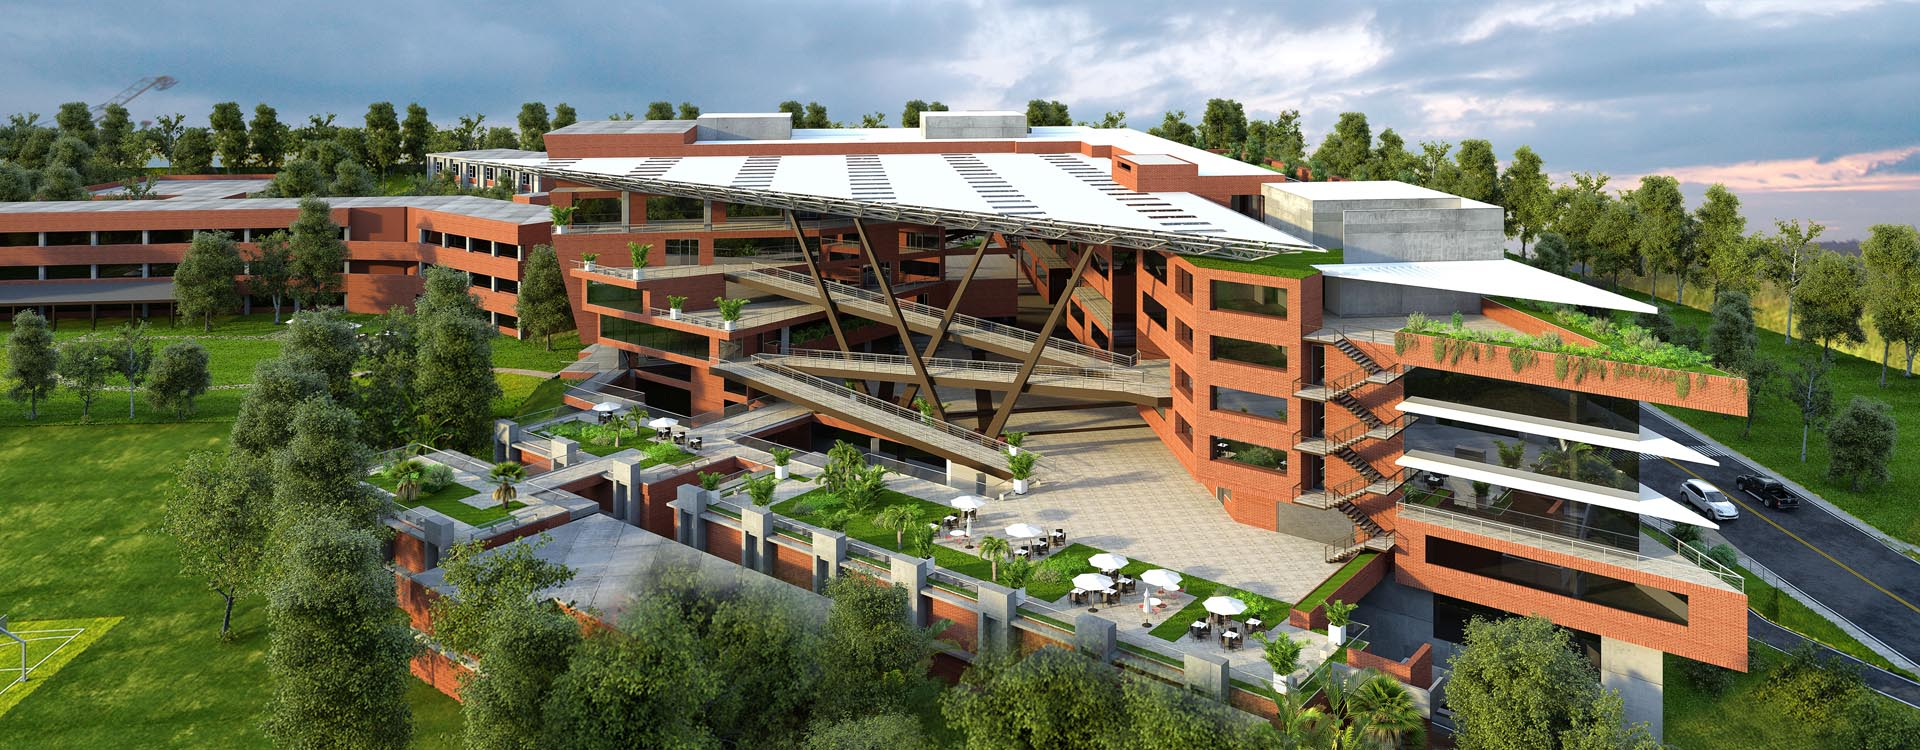
\includegraphics[height=13.25cm]{plantilla/portadacit.jpg}}
    	\makebox[\textwidth]{
    		\begin{overpic}[height=13.25cm]{\imagenportada}
     		\put(63,0){
\includegraphics[height=1.15in]{plantilla/fondologo_grande.png}}  
  			\put(64.5,2){
\includegraphics[height=0.55in]{plantilla/logoUVGblanco.eps}} 
        	\end{overpic}
    	}
    	%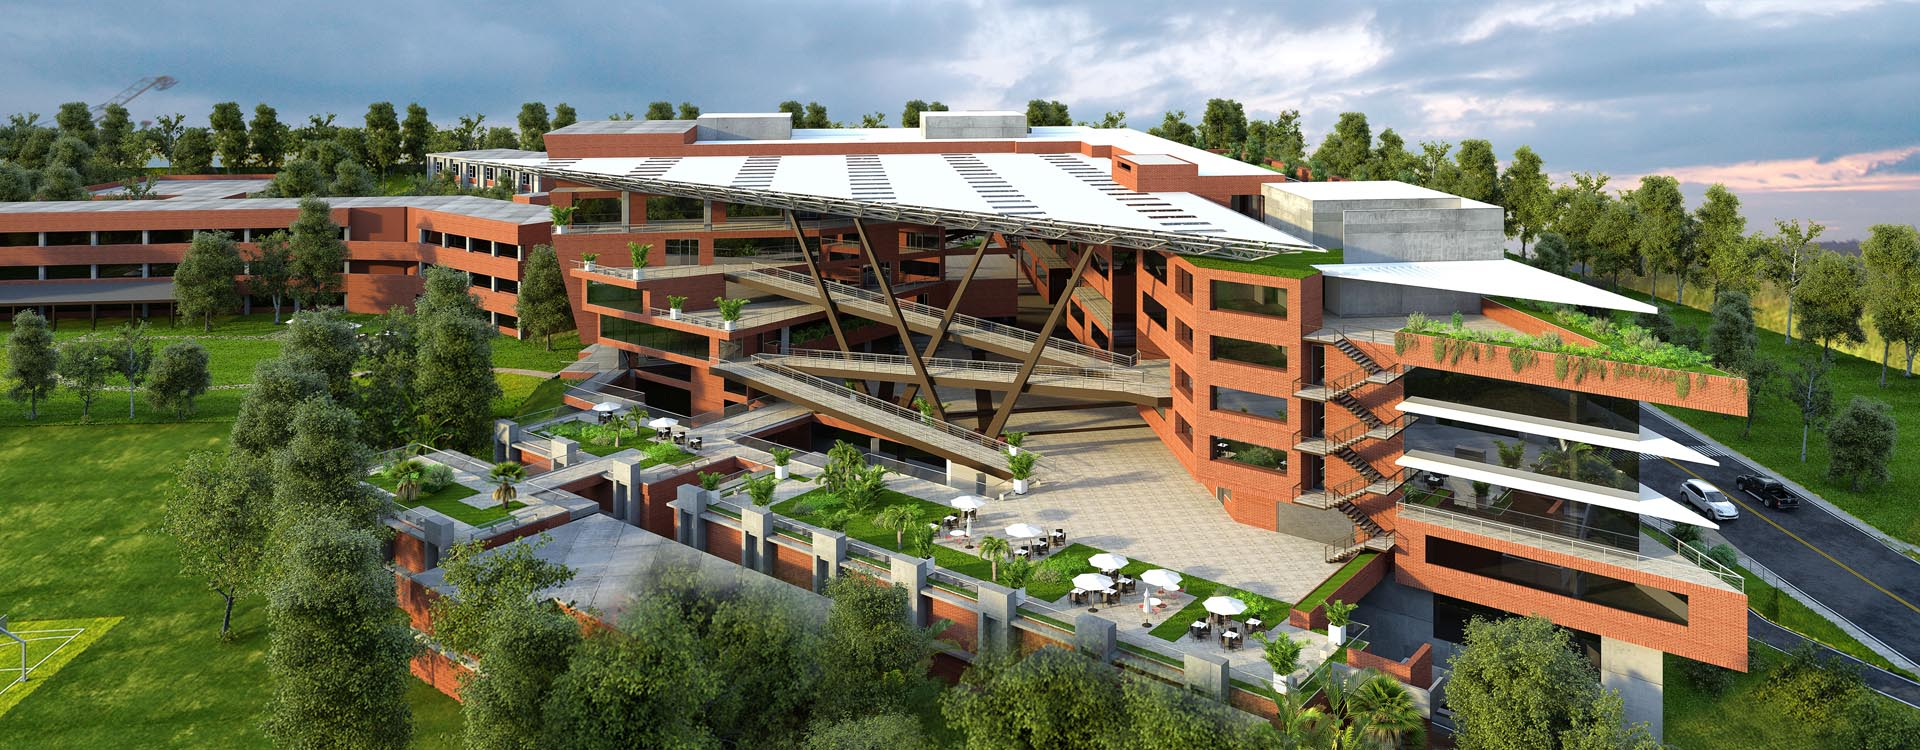
\includegraphics[height=13.25cm]{plantilla/portadacit.jpg}
	\end{figure}
	\restoregeometry
\fi


% ================================================================================
% PRIMERA PÁGINA
% ================================================================================

\newpage
\thispagestyle{empty}
\pagecolor{white}
\mbox{}
\newpage

\ifdefined\CAPcaratula
	\newpage
%     \cleardoublepage\phantomsection
%     \pdfbookmark{Carátula}{toc}
	\pagecolor{white}
	\color{black}
	\setcounter{page}{1}
	\pagenumbering{roman}
	\thispagestyle{empty}
	\begin{center}
		\LARGE UNIVERSIDAD DEL VALLE DE GUATEMALA\\
		\LARGE Facultad de \uvgfacultad \\[0.75cm]
	\end{center}
	\begin{figure}[h]
		\begin{center}
		
\includegraphics[height=5.5 cm]{plantilla/escudoUVGnegro.eps}
		\vspace{0.5in}
		\end{center}
	\end{figure}
	\begin{center}
		\LARGE \textbf{\titulotesis} 
		\vfill
		\vfill
		\Large Trabajo de graduación en modalidad megaproyecto tecnológico presentado por \\
		\Large \nombreestudiante \\
		\Large Para optar al grado académico de Licenciada en \uvgcarrera \\
		\vfill
		\large Guatemala, \mesentrega del \anoentrega
	\end{center}
\fi

% ================================================================================
% HOJA DE FIRMAS
% ================================================================================

\newpage
\thispagestyle{empty}
\mbox{}
\newpage

\ifdefined\CAPfirmas
	\newpage
	\thispagestyle{empty}
	\vspace*{0.5in}
	\large Vo.Bo.:\\[1cm]
	\begin{center}
		(f) \rule[1pt]{4 in}{1pt}\\
		\nombreasesor
	\end{center}
	\vspace{1in}

	Tribunal Examinador:\\[1cm]
	\begin{center}
		(f) \rule[1pt]{4 in}{1pt}\\
		\nombreasesor \\[1in]
		(f) \rule[1pt]{4 in}{1pt}\\
		\nombreprimerex \\[1in]
		(f) \rule[1pt]{4 in}{1pt}\\
		\nombresegundoex
	\end{center}
	\vspace{1in}

	Fecha de aprobación: \fechaaprobacion.
	\normalsize
\fi

% ================================================================================
% CONTENIDO DEL TRABAJO
% ================================================================================
% PREFACIO
% --------------------------------------------------------------------------------
\newpage
\thispagestyle{empty}
\mbox{}
\newpage

\ifdefined\CAPprefacio
	\newpage
	\cleardoublepage\phantomsection
    \chapter*{Prefacio}
    \ifdefined\parpordefecto
    	\defaultparformat{prefacio}
    \else
    	El proyecto \textit{Señas Chapinas: Traductor de LENSEGUA} emerge como una respuesta innovadora ante la necesidad crítica de desarrollar herramientas tecnológicas que faciliten la inclusión efectiva de la comunidad sorda en Guatemala. Este proyecto no solo busca abordar las barreras de comunicación existentes, sino también empoderar a las personas sordas para que puedan participar plenamente en todos los aspectos de la vida social, educativa y profesional.

La integración de tecnologías de inteligencia artificial en este contexto representa un avance significativo en la manera en que abordamos los desafíos de accesibilidad y comunicación. Al desarrollar un traductor de LENSEGUA (Lengua de Señas Guatemalteca) basado en modelos de lenguaje avanzados, este proyecto establece un precedente importante en la aplicación de soluciones tecnológicas para resolver problemáticas sociales complejas. La iniciativa no solo busca facilitar la comunicación cotidiana, sino también promover una mayor comprensión y apreciación de la riqueza lingüística y cultural de la comunidad sorda guatemalteca.
    \fi
    \addcontentsline{toc}{chapter}{Prefacio}
\fi

% AGRADECIMIENTOS
% --------------------------------------------------------------------------------
\newpage
\thispagestyle{empty}
\mbox{}
\newpage 
\ifdefined\CAPagradecimientos
	\newpage
    \cleardoublepage\phantomsection
	\chapter*{Agradecimientos}
	\ifdefined\parpordefecto
    	\defaultparformat{agradecimientos}
    \else
    	Queremos expresar nuestro más sincero agradecimiento a todas las personas que han contribuido a la realización de este proyecto, cada una de las cuales ha sido fundamental en su desarrollo.

Primero, expresamos nuestra gratitud a nuestros asesores, los Ingenieros Dennis Aldana, Miguel Novella, Luis Alberto Suriano y Javier Fong, profesores de la Universidad del Valle, por su invaluable guía y apoyo a lo largo de todo el proceso de investigación y redacción de este trabajo. Su experiencia y dirección experta fueron fundamentales para superar los retos académicos y prácticos de este proyecto.

Estamos profundamente agradecidos con ASEDES, especialmente con Niurka Waleska Bendfeldt Rosada y Alain de León, por proporcionarnos materiales, entrevistas y otros recursos necesarios para llevar a cabo este trabajo. Su colaboración fue indispensable para entender mejor las necesidades y desafíos de la comunidad sorda.

Nuestro reconocimiento a las alumnas practicantes de ASEDES: Evelyn Cacao, Any Max y Ruth Amézquita, quienes generosamente permitieron que las grabáramos mientras realizaban señas, contribuyendo significativamente a la autenticidad y calidad del contenido de este proyecto.

Agradecemos la colaboración de la profesora Pamela Ramírez, quien contribuyó en el diseño del logo de la aplicación. Su trabajo fue esencial, ya que el logo desempeña un papel crucial en la identidad visual y la coherencia del diseño de la aplicación.

Finalmente, un agradecimiento especial a Antonio Barrientos, Director General de En-Señas, y a Gabriela Velázquez, maestra de En-Señas, por su apertura y disposición para compartir su conocimiento y experiencia, las cuales fueron cruciales para este proyecto.

A todos ustedes, nuestro más profundo respeto y gratitud por su apoyo y contribuciones.
    \fi 
	\addcontentsline{toc}{chapter}{Agradecimientos}
\fi

% ÍNDICE GENERAL
% --------------------------------------------------------------------------------
\newpage
\thispagestyle{empty}
\mbox{}
\newpage

\ifdefined\CAPindice
	\newpage
    %\cleardoublepage\phantomsection
	\renewcommand{\contentsname}{Índice}
    \phantomsection
    \pdfbookmark{\contentsname}{toc}
	\tableofcontents
\fi

% LISTADO DE FIGURAS
% --------------------------------------------------------------------------------

\ifdefined\CAPfiguras
	\newpage
    \cleardoublepage\phantomsection
	\renewcommand{\listfigurename}{Lista de Figuras}
	\listoffigures
	\addcontentsline{toc}{chapter}{Lista de Figuras}
\fi


% RESUMEN
% --------------------------------------------------------------------------------
\newpage
\thispagestyle{empty}
\mbox{}
\newpage

\ifdefined\CAPresumen
	\newpage
    \cleardoublepage\phantomsection
	\chapter*{Resumen}
	\ifdefined\parpordefecto
		\defaultparformat{resumen}
	\else
		``Señas Chapinas'' es un proyecto innovador que responde a la necesidad crítica de mejorar la comunicación para los usuarios de LENSEGUA en Guatemala. Desarrollada como una aplicación móvil para Android, esta herramienta utiliza tecnologías de visión por computadora y aprendizaje profundo para traducir la lengua de señas guatemalteca a texto con gramática española. La aplicación está especialmente diseñada para cubrir vocabulario esencial, tanto para situaciones cotidianas como de emergencia, facilitando así las interacciones diarias y elevando la calidad de vida de la comunidad sorda.

A lo largo del desarrollo de ``Señas Chapinas'', se implementaron metodologías de diseño centradas en el usuario para crear una interfaz que no solo es funcional y accesible, sino también culturalmente relevante, reflejando la identidad guatemalteca para conectar profundamente con los usuarios. Este enfoque asegura que la aplicación no solo sea una herramienta de traducción, sino también un medio para fomentar la inclusión y el entendimiento cultural.

La colaboración activa con la comunidad sorda ha sido vital en todas las etapas del proyecto, desde la concepción hasta la implementación. Esta cooperación ha permitido que ``Señas Chapinas'' se desarrolle no solo como una solución tecnológica, sino como un recurso comunitario que promueve una mayor inclusión social y entendimiento.

Con ``Señas Chapinas'', se espera establecer un precedente para futuras innovaciones en tecnologías accesibles, demostrando cómo las herramientas adecuadamente diseñadas pueden superar barreras significativas y mejorar la interacción social dentro y fuera de la comunidad sorda.
	\fi
	\addcontentsline{toc}{chapter}{Resumen}
\fi

% INTRODUCCIÓN
% --------------------------------------------------------------------------------
\newpage
\thispagestyle{empty}
\mbox{}
\newpage 

\ifdefined\CAPintroduccion
	\newpage
	\pagenumbering{arabic}
	\setcounter{page}{1}
	\chapter{Introducción}
	\ifdefined\parpordefecto
		\defaultparformat{introduccion}
	\else
		Este proyecto surge de la necesidad de superar las barreras de comunicación para los usuarios de LENSEGUA. ``Señas Chapinas'' es una iniciativa que consiste en el desarrollo de una aplicación móvil para Android, diseñada para traducir lengua de señas a texto utilizando tecnologías avanzadas como visión por computadora y aprendizaje profundo. Con un enfoque en el vocabulario esencial para la vida cotidiana y situaciones de emergencia, la aplicación tiene como objetivo facilitar las interacciones diarias y mejorar la calidad de vida de la comunidad sorda. 

La aplicación combina un diseño intuitivo y culturalmente relevante con una infraestructura tecnológica eficiente y segura, capaz de gestionar y procesar datos de manera efectiva. Esto asegura una experiencia de usuario accesible, funcional y preparada para crecer en el futuro, convirtiéndose en un recurso valioso para la comunicación y la integración social.

En colaboración con la comunidad sorda y con base en una retroalimentación constante, ``Señas Chapinas'' busca ser más que una aplicación; aspira a ser un recurso valioso que no solo mejore la comunicación, sino que también fomente una mayor inclusión y entendimiento dentro de la sociedad guatemalteca.

	\fi
\fi

% OBJETIVOS
% --------------------------------------------------------------------------------
\newpage
\thispagestyle{empty}
\mbox{}
\newpage

\ifdefined\CAPobjetivos
	\newpage
	\chapter{Objetivos}
	\ifdefined\parpordefecto
		\defaultparformat{objetivos}
	\else
		\section{Objetivo General}

Diseñar y desarrollar \textit{Señas Chapinas}, una aplicación para dispositivos Android que sea capaz de traducir la lengua de señas guatemalteca (LENSEGUA) a texto gramaticalmente correcto en español, haciendo uso de modelos avanzados de visión por computadora y procesamiento de lenguaje natural, junto con una infraestructura de red segura y eficiente.


\section{Objetivos Específicos}
\begin{itemize}

\item Desarrollar un sistema de visión por computadora destinado al reconocimiento de la lengua de señas de Guatemala. Para ello, se creará un conjunto de datos que incluya al menos veinticinco palabras de esta lengua, seleccionando aquellas que permitan formar una amplia variedad de frases de uso cotidiano.

\item Adaptar un \textit{large language model}, específicamente GPT-3.5-Turbo, para que asimile la gramática de LENSEGUA, permitiéndole interpretar oraciones que utilicen dicha gramática y las escriba correctamente en español.

\item Desarrollar una herramienta basada en LLaMA que sea capaz de comprender la gramática de LENSEGUA y generar interpretaciones coherentes en español a partir de oraciones estructuradas en dicha gramática. 

\item Configurar un servidor seguro y eficiente que optimice el uso de recursos para administrar modelos de inteligencia artificial, procesar videos, y ofrecer un ambiente accesible para pruebas y despliegues mediante APIs.

\item Realizar una investigación de mercado y entrevistas para comprender necesidades, diseñar flujos e interfaces intuitivas, y desarrollar la aplicación \textit{Señas Chapinas} integrando servicios externos para la traducción de LENSEGUA.

\end{itemize}
	\fi
\fi

% JUSTIFICACIÓN
% --------------------------------------------------------------------------------
\newpage
\thispagestyle{empty}
\mbox{}
\newpage

\ifdefined\CAPjustificacion
	\newpage
	\chapter{Justificación}
	\ifdefined\parpordefecto
		\defaultparformat{justificacion}
	\else
		La comunicación es un derecho fundamental y un pilar esencial para la interacción humana, indispensable en la educación, el trabajo y la participación activa en la sociedad \cite{NacionesUnidas2024}. En Guatemala, según datos del Conadi (Consejo Nacional para la Atención de las Personas con Discapacidad) recogidos hasta marzo de 2021, existían entre 240,000 y 250,000 personas que utilizaban la lengua de señas como su principal herramienta de comunicación \cite{Conadi2021}. Sin embargo, las barreras comunicativas continúan limitando la interacción entre personas sordas y oyentes, restringiendo su acceso igualitario a oportunidades sociales y laborales. Ante esta realidad, "Señas Chapinas" surge como una solución innovadora para superar estas barreras.

Aprovechando la amplia adopción de teléfonos inteligentes en Guatemala \cite{Xie2023}, donde la mayoría de estos dispositivos operan con el sistema Android \cite{Xie2023}, este proyecto busca desarrollar una aplicación móvil que actúe como un puente de comunicación eficiente y accesible. La aplicación pretende fortalecer la autonomía de las personas sordas en diversas situaciones cotidianas y de emergencia, promoviendo al mismo tiempo el uso de LENSEGUA. Además, se sustenta en un marco legal favorable, como el Decreto del Congreso de la República de Guatemala Número 3-2020, que reconoce la Lengua de Señas de Guatemala \cite{CongresoGuatemala2022}.


Un aspecto clave de este proyecto es la integración de diversos componentes tecnológicos para que funcionen como una unidad cohesiva en lugar de elementos independientes. Esta integración resulta crucial para conectar las capacidades de los modelos de inteligencia artificial, la funcionalidad de la aplicación móvil y la infraestructura del servidor.

El propósito de "Señas Chapinas" es fomentar la inclusión laboral, facilitar el acceso a servicios esenciales y promover las interacciones sociales, contribuyendo al enriquecimiento de la comunidad guatemalteca.
Es por ello que este proyecto representa un avance significativo hacia la construcción de una sociedad que valora la diversidad y garantiza igualdad de oportunidades para todos, utilizando tecnología móvil para superar las barreras de comunicación de manera eficiente y efectiva.





	\fi
\fi

% MARCO TEÓRICO
% --------------------------------------------------------------------------------
\newpage
\thispagestyle{empty}
\mbox{}
\newpage 

\ifdefined\CAPmarcoteorico
	\newpage
	\chapter{Marco Teórico}
	\ifdefined\parpordefecto
		\defaultparformat{marco_teorico}
	\else
		\section{Lengua de Señas}
Desde tiempos remotos, las personas con discapacidad auditiva han enfrentado significativos desafíos para expresarse, lo que les llevó a desarrollar su propio sistema de comunicación. Así surgió la lengua de señas, un conjunto estructurado de gestos visuales que permite a la comunidad sorda expresar ideas y emociones. Esta lengua, al igual que otras, está regida por normas lingüísticas establecidas por comunidades sordas \cite{MarzoPena2022}.

\subsection{Historia de la lengua de señas}
La lengua de señas se desarrolló de manera independiente por la comunidad sorda para satisfacer sus necesidades comunicativas. Históricamente estigmatizada y mal entendida, era considerada un lenguaje de gestos simple hasta que investigaciones realizadas en 1960 por William Stokoe revelaron su capacidad para expresar ideas complejas y estructuradas \cite{RodriguezVelasquezSF}.

En el siglo XVIII, el Abad Charles-Michel de L’Epée fundó la primera escuela pública para sordos, marcando un cambio trascendental en la educación de esta comunidad, utilizando la lengua de señas como principal medio de enseñanza. Este avance no solo facilitó la comunicación y el aprendizaje, sino que también permitió que los sordos desempeñaran roles activos como educadores. La metodología de L’Epée se expandió internacionalmente, influyendo en la creación de escuelas y en el desarrollo de nuevas lenguas de señas \cite{RodriguezVelasquezSF}.

Durante los siglos XIX y XX, las lenguas de señas ganaron reconocimiento como sistemas lingüísticos completos y estructurados, capaces de expresar una gama completa de ideas y emociones. En el siglo XX, el reconocimiento de los derechos lingüísticos de las comunidades sordas se amplió significativamente, afirmando la importancia de las lenguas de señas como herramientas educativas y culturales esenciales \cite{RodriguezVelasquezSF}.

A raíz de la necesidad de comunicación en las comunidades sordas, cada país ha desarrollado su propia lengua de señas, integrando a menudo estructuras de lenguas de señas extranjeras, como el \textit{American Sign Language (ASL)}, así como señas locales únicas. Esto ha dado lugar a que cada país, e incluso regiones dentro de los mismos, tengan su propia lengua de señas con estructuras gramaticales y léxicos distintos \cite{RuizVilla2022}.

\subsection{Lengua de Señas en la Actualidad}
En la actualidad, la lengua de señas se está adaptando a un entorno globalizado y tecnológicamente avanzado, donde las necesidades comunicativas evolucionan constantemente. Estos cambios han impulsado la creación de legislaciones, políticas, formación de asociaciones y el desarrollo de nuevas tecnologías destinadas a minimizar las barreras comunicativas. Un ejemplo significativo es la iniciativa de las Naciones Unidas al proclamar el 23 de septiembre como Día Internacional de las Lenguas de Señas, enfatizando la importancia de estas lenguas \cite{Parada2022}.

Sin embargo, a pesar de estos avances, persisten desafíos significativos. La falta de estandarización de las lenguas de señas a nivel global requiere que las personas aprendan la lengua de señas específica de cada comunidad, lo cual impide la existencia de una forma de comunicación internacional uniforme \cite{RuizVilla2022}.

Además, la lengua de señas, a menudo catalogada como una lengua minoritaria, es aprendida solamente por una pequeña fracción de la población sin discapacidades auditivas. Esta limitada difusión crea una brecha de comunicación significativa, contribuyendo a la marginación de la comunidad sorda y limitando su participación plena en actividades sociales y económicas. Esto subraya la necesidad de una mayor educación y sensibilización sobre la lengua de señas para promover una verdadera inclusión \cite{MelendezLabrador2021}.

\section{Lengua de Señas de Guatemala (LENSEGUA)}

\subsection{Historia}
La Lengua de Señas de Guatemala (LENSEGUA) ha evolucionado como una herramienta vital de comunicación para la comunidad sorda guatemalteca. Aunque su desarrollo específico ha sido menos documentado en comparación con lenguas de señas de otros países, LENSEGUA ha sido influenciada tanto por ``Señas Caseras''\footnote{Se conoce como ``Señas Caseras'' al sistema de comunicación que utilizan los niños sordos, que no han sido expuestos a la lengua de señas, con padres oyentes para poder comunicarse y desenvolverse en el ámbito familiar \cite{EnSenasCultura}.} de diferentes departamentos del país como por interacciones con lenguas de señas de otros países \cite{Aroche2022} \cite{EndangeredLanguages}.


Antes de la formalización del uso de LENSEGUA, no existía un manual estandarizado que facilitara el aprendizaje de la lengua de señas guatemalteca. Hoy en día de hecho todavía existen diferencias entre las señas utilizadas en los departamentos del país. Sin embargo, en julio de 2001, el Comité Pro Ciegos y Sordos de Guatemala, una institución pionera en la educación y rehabilitación de personas con discapacidad auditiva, publicó el primer manual oficial para el aprendizaje de LENSEGUA. Este manual representó un avance crucial en la estandarización y enseñanza de la lengua de señas, proporcionando un recurso esencial para los estudiantes, profesionales y la comunidad en general interesada en aprender este método de comunicación \cite{deLeon2021}.

\subsection{Legislación}
En términos legislativos, Guatemala ha hecho avances significativos en la última década. En 2020 el Congreso de la República de Guatemala mediante el Decreto 3-2020, reconoce oficialmente la Lengua de Señas de Guatemala como la lengua oficial para la comunicación en lengua de señas dentro del país. Este marco legal fue el resultado de los esfuerzos conjuntos de varias asociaciones que abogaron por su formalización, destacando la importancia de reconocer y apoyar la comunicación para las personas sordas en Guatemala \cite{CongresoGuatemala2020} .

El Decreto establece que todas las instituciones públicas y privadas deben garantizar la inclusión de LENSEGUA como parte de su comunicación y servicios. Además, se promueve la educación bilingüe (español y LENSEGUA) en las escuelas que atienden a estudiantes sordos, asegurando así su derecho a una educación equitativa y accesible \cite{CongresoGuatemala2020}.

Este reconocimiento no solo valida a LENSEGUA como una lengua completa y estructurada, sino que también impulsa la creación de políticas y programas destinados a mejorar la accesibilidad en todos los aspectos de la vida pública para la comunidad sorda, desde la educación hasta el acceso a los servicios de salud y legales. El Decreto promueve la inclusión y asegura que las personas con discapacidad auditiva tengan acceso a la educación y la información en lengua de señas, libre de cualquier discriminación \cite{CongresoGuatemala2020}.

\subsection{Aprendizaje y Recursos}
LENSEGUA se puede aprender en varias instituciones y a través de recursos en línea que buscan facilitar el acceso y la difusión de esta lengua. Entre las principales entidades que ofrecen cursos y formación en LENSEGUA están \cite{LenseguaSF}:

\begin{itemize}
    \item ASEDES (Asociación Educativa para el Sordo)
    \item ASORGUA (Asociación de Sordos de Guatemala)
    \item Benemérito Comité Prociegos y Sordos de Guatemala
    \item En-Señas Guatemala
    \item CESGUA (Coordinación de Educación y Servicios en Guatemala)
    \item INTERGUA (Coordinación de intérpretes de lengua de señas de Guatemala)
    \item ANDYSISC (Servicios de interpretación profesional de Lengua de Señas)
    \item FUNDAL
    \item ONG Sordos Latinos Guatemala
\end{itemize}

Estas organizaciones no solo proporcionan educación en LENSEGUA, sino que facilitan una serie de conferencias y talleres impartidos por especialistas para personas con discapacidad auditiva \cite{LenseguaSF}.

\subsection{Gramática y Estructura}
La gramática y estructura de LENSEGUA reflejan una vasta complejidad lingüística que permite a los usuarios expresar una amplia gama de conceptos y emociones. Este sistema de comunicación es completo con su propia sintaxis, léxico y reglas gramaticales. Aquí se describen algunas de las características distintivas de LENSEGUA \cite{EnSenasCultura}  \cite{EnSenasGramatica} \cite{EnSenasTecnicas}  :

\begin{itemize}
    \item \textbf{Morfología}: La morfología en LENSEGUA utiliza modificadores manuales y no manuales para alterar el significado de los signos básicos, incluyendo modificaciones para indicar número, tiempo, aspecto, y otros atributos gramaticales.
    \begin{itemize}
        \item El signo para ``comer" podría modificarse para expresar ``comer mucho" mediante la repetición del signo o cambios en la expresión facial.
    \end{itemize}
    \item \textbf{Ausencia de género y artículos}: Como en muchas lenguas de señas, LENSEGUA no utiliza género gramatical ni artículos.
    \begin{itemize}
        \item Español: ``la casa'', ``el perro''.
        \item LENSEGUA signa ``casa'' y ``perro'' sin modificadores adicionales.
    \end{itemize}
    \item \textbf{No Uso de Preposiciones}: LENSEGUA omite preposiciones, que en español son cruciales para las relaciones espaciales o temporales. La relación se establece a través del contexto y la configuración de los signos.
    \begin{itemize}
        \item Español: ``en la casa''.
        \item LENSEGUA: se usa gesto para indicar la ubicación relativa y el signo de casa.
    \end{itemize}
    \item \textbf{Omisión de Signos de Puntuación y Mayúsculas}: LENSEGUA no utiliza signos de puntuación ni mayúsculas. La escritura refleja una secuencia continua de signos, que se diferencia notablemente de la estructura del español.
    \begin{itemize}
        \item LENSEGUA: ``Disculpar mi hija no llega colegio porque muy enferma tiene tos casa tomar medicinas''.
    \end{itemize}
    \item \textbf{Verbos No Conjugados}: En LENSEGUA, los verbos no se conjugan. El tiempo y el aspecto se indican con signos específicos al principio de la frase o a través de la expresión facial.
    \begin{itemize}
        \item Español: ``Yo estoy comiendo''.
        \item LENSEGUA: se signa ``yo comer''.
    \end{itemize}
    \item \textbf{Orden Gramatical}: El orden gramatical típico en LENSEGUA es Tiempo, Lugar, Sujeto, Objeto, Verbo (TLSOV), diferente al orden Sujeto, Verbo, Objeto (SVO) del español. Este orden facilita que el contexto temporal y espacial quede establecido claramente al inicio.
    \begin{itemize}
        \item Español: ``Yo ayer jugué futbol''.
        \item LENSEGUA: se signa ``ayer yo fútbol jugar''.
    \end{itemize}
\end{itemize}

\section{Diseño de Interfaz de Usuario (UI)}
\subsection{Definición de UI (Interfaz de Usuario)}
El diseño de la interfaz de usuario (UI por sus siglas en ingles, \textit{User Interface}) se dedica a la creación de los elementos visuales e interactivos de un producto digital. En esencia, se trata de diseñar lo que los usuarios ven en sus pantallas \cite{OrtegaSF}.

La interfaz de usuario determina en gran medida las primeras impresiones que tienen estos acerca de un negocio o producto. Cuando los usuarios pueden navegar fácilmente por una interfaz y completar las tareas deseadas, no solo mejora su experiencia, sino que también beneficia al negocio en general. Cuanto más visualmente atractiva y acogedora sea una interfaz, más probable es que atraiga a los usuarios y los motive a explorar más \cite{OrtegaSF}.

\subsection{Elementos de la Interfaz de Usuario}
Los elementos de la UI son los componentes básicos de las aplicaciones y sitios web con los que los usuarios interactúan. Estos elementos son esenciales para el desarrollo de funcionalidades óptimas y una experiencia de navegación agradable. Los elementos UI se agrupan en tres categorías principales \cite{OrtegaSF}:

\begin{itemize}
    \item \textbf{Elementos de entrada}: Permiten a los usuarios ingresar información en el sistema y, en ocasiones, son parte del proceso de validación de entrada. Los elementos de entrada más comunes incluyen \cite{OrtegaSF}:
    \begin{itemize}
        \item Listas desplegables
        \item Campos de texto o contraseña
        \item Selectores de fecha
        \item Casillas de verificación
        \item Diálogos de confirmación
    \end{itemize}
    \item \textbf{Elementos de salida}: Muestran los resultados basados en las entradas del usuario y las operaciones previas. Ejemplos de elementos de salida son \cite{OrtegaSF}:
    \begin{itemize}
        \item Alertas
        \item Mensajes de éxito
        \item Mensajes de error
    \end{itemize}
    \item \textbf{Elementos auxiliares}: Proporcionan información adicional al usuario y mejoran la navegación. Estos elementos se dividen en tres subcategorías \cite{OrtegaSF}:
    \begin{itemize}
        \item \textbf{Elementos de navegación}: Facilitan el desplazamiento a través del producto digital \cite{OrtegaSF}. Algunos ejemplos son:
        \begin{itemize}
            \item Menús de navegación
            \item Listas de enlaces
        \end{itemize}
        \item \textbf{Elementos informativos}: Incluyen referencias que ayudan a utilizar o comprender el producto digital \cite{OrtegaSF}. Ejemplos son:
        \begin{itemize}
            \item Iconos
            \item Notificaciones
        \end{itemize}
        \item \textbf{Elementos de grupos o contenedores}: Ayudan a organizar y mantener los componentes del producto juntos \cite{OrtegaSF}. Ejemplos incluyen:
        \begin{itemize}
            \item Barras laterales
            \item Contenedores de contenido
        \end{itemize}
    \end{itemize}
\end{itemize}

\subsection{Estándares de Diseño}
\subsubsection{Tamaño y Posición de Botones}
El tamaño de los objetos táctiles en una aplicación móvil es crucial, ya que afecta directamente la facilidad con la que los usuarios pueden interactuar con la interfaz. Si los botones no tienen un tamaño y espacio óptimos, los usuarios podrían no alcanzar su objetivo o presionar el botón equivocado \cite{Bustos2022}.

Investigaciones sobre el tamaño y el espaciado de los botones han establecido estándares que funcionan para la mayoría de los usuarios. Los estudios encontraron que los usuarios tienen la menor precisión táctil en botones de menos de 42 píxeles, los cuales se usan generalmente para funciones de baja prioridad. La mayor precisión se encontró en botones de entre 42 y 72 píxeles. Por ello, se utilizan botones de aproximadamente 60 píxeles para funciones de prioridad media, mientras que los de más de 72 píxeles se reservan para funciones de alta prioridad, asegurando así la accesibilidad para todos los usuarios \cite{Anthony2019}.

\begin{figure}[H]
    \centering
    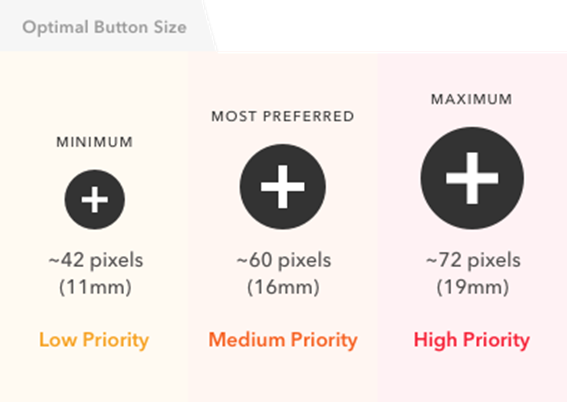
\includegraphics[width=0.6\linewidth]{figuras/optimal_button_size.png}
    \caption{Tamaño óptimo de botones según su prioridad}
    \label{fig:botones_optimos}
\end{figure}

Además del tamaño, existen ciertos márgenes y áreas táctiles recomendadas alrededor de los botones para garantizar que sean fácilmente accesibles y utilizables. Estos márgenes aseguran que haya suficiente espacio alrededor de los botones para evitar errores de pulsación. Dependiendo del tamaño del botón, se recomienda un margen de 12 a 24 píxeles para botones grandes, de 24 a 36 píxeles para botones medianos y de 36 a 48 píxeles para botones pequeños \cite{Anthony2019}. 

\begin{figure} [H]
    \centering
    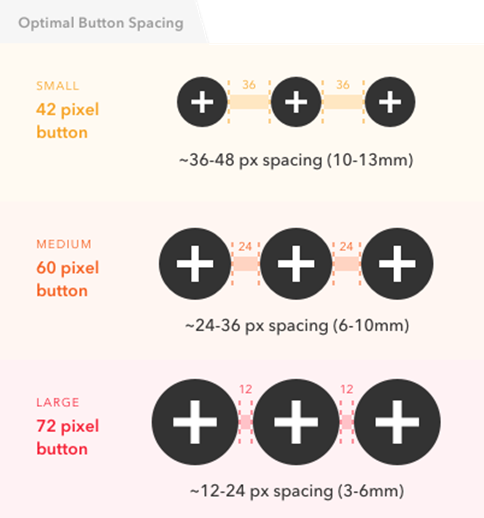
\includegraphics[width=0.5\linewidth]{figuras/optimal_space_buttons.png}
    \caption{Espaciado óptimo de botones según su tamaño}
    \label{fig:esapcio_optimo}
\end{figure}

Asimismo, la ubicación de los botones es fundamental para la usabilidad. Los usuarios están acostumbrados a interactuar con dispositivos digitales a lo largo del día y tienden a buscar ciertos elementos en ubicaciones predecibles. Por esta razón, es importante posicionar los botones en lugares donde los usuarios esperan encontrarlos, como en la parte inferior de la pantalla para acciones frecuentes o en la esquina superior derecha para opciones adicionales. Esta previsibilidad mejora la eficiencia y reduce la frustración del usuario \cite{Pickaso2022}.


\subsubsection{Diseño Responsivo}
El diseño responsivo es crucial para aplicaciones móviles, ya que asegura que la interfaz se adapte a diferentes tamaños de pantalla y resoluciones \cite{Becos2024}.

Dado que las pantallas de los dispositivos móviles varían en densidad, con más píxeles por pulgada en pantallas de mayor resolución, es importante utilizar píxeles independientes de la densidad (dp) para definir las dimensiones de los elementos de la interfaz. Esto asegura que los elementos mantengan su tamaño y proporción adecuados en diferentes dispositivos, proporcionando uniformidad y coherencia visual \cite{Pickaso2022}.

\subsubsection{Principios de Diseño}
Hay una serie de principios de diseño de interfaz para lograr que el producto digital satisfaga al cliente final \cite{AnonimoUX}.

\begin{itemize}
    \item \textbf{Simplicidad}: Es crucial evitar elementos innecesarios que puedan causar confusión \cite{AnonimoUX}.
    \item \textbf{Consistencia}: Al emplear elementos comunes en la interfaz de usuario, los usuarios se sienten más cómodos y familiarizados con el diseño, lo que facilita el uso del producto digital \cite{AnonimoUX}.
    \item \textbf{Jerarquía y manejo de espacios}: La disposición y estructuración de los elementos según su importancia ayuda a dirigir la atención del usuario a la información más relevante. Agrupar elementos relacionados crea una relación visual y mejora la comprensión del contenido \cite{AnonimoUX}.
    \item \textbf{Color y tipografía}: El color es esencial en el diseño de interfaces. Ajustar la saturación, luz y contraste del color en el diseño destaca elementos importantes y facilita la navegación. Asimismo, se utilizan diferentes tamaños, fuentes y disposiciones del texto para mejorar la legibilidad y jerarquía visual \cite{AnonimoUX}.
\end{itemize}

\subsubsection{Paleta de Colores}
Los colores desempeñan un papel fundamental en el diseño de interfaces de usuario, ya que no solo aportan personalidad y estilo al producto digital, sino que también influyen en la percepción y emociones del usuario \cite{EspacioUXSF}.

Una paleta de colores bien diseñada ayuda a los usuarios a comprender rápidamente la importancia y la relación entre diferentes elementos en la interfaz, como las llamadas a la acción o la información crítica. Al asignar colores específicos a distintas categorías o secciones, los usuarios pueden identificar fácilmente su ubicación en la interfaz y cómo navegar dentro de ella \cite{EspacioUXSF}.

La paleta de colores se elige para evocar emociones específicas que se alineen con los objetivos del diseño. Por ejemplo, los colores cálidos como el rojo y el naranja pueden provocar sensaciones de urgencia o excitación, lo que los hace ideales para botones de compra o alertas. En contraste, los colores fríos como el azul y el verde pueden inducir sensaciones de tranquilidad y confianza, siendo perfectos para páginas de inicio o secciones de información \cite{EspacioUXSF}.

Es esencial que la paleta de colores tenga en cuenta la legibilidad y la visibilidad, cumpliendo con los estándares de contraste y asegurando que la información sea clara para todos los usuarios \cite{EspacioUXSF}.

\subsubsection{Selección de Tipografía}
Al igual que la paleta de colores, la elección de una tipografía tiene un impacto significativo en el diseño de un producto digital. La tipografía moldea la manera en que se percibe y comprende la información visual. Elementos tipográficos como el tipo de letra, su tamaño y color tienen la capacidad de transmitir diversos significados y causar distintas respuestas emocionales \cite{CamaraSevilla2023}.

Una tipografía bien elegida mejora y facilita la comprensión y asimilación de la información por parte de los usuarios. Por ejemplo, una fuente en negrita y con letras mayúsculas puede transmitir fuerza y determinación, mientras que una tipografía delicada y manuscrita puede evocar elegancia y sofisticación. En contraste, una tipografía inadecuada puede dificultar la lectura, causar fatiga visual e incluso generar confusión o frustración en el usuario \cite{CamaraSevilla2023}.

Las tipografías se pueden clasificar según sus características:

\begin{itemize}
    \item \textbf{Fuentes Serif}: Estas fuentes se caracterizan por tener pequeños remates en los extremos de las letras, transmitiendo una sensación de formalidad. Ejemplos populares incluyen Times New Roman y Georgia \cite{CamaraSevilla2023}.
    \item \textbf{Fuentes Sans Serif}: Carecen de remates, lo que les confiere una apariencia más moderna y limpia. Se utilizan comúnmente en proyectos digitales. Ejemplos comunes son Arial, Helvetica y Calibri \cite{CamaraSevilla2023}.
    \item \textbf{Fuentes Script o Manuscritas}: Estas fuentes imitan la escritura a mano y suelen transmitir una sensación de personalización y creatividad. Ejemplos incluyen Brush Script y Pacifico \cite{CamaraSevilla2023}.
    \item \textbf{Fuentes Decorativas}: Son variadas y altamente estilizadas, utilizadas con fines ornamentales y para llamar la atención. Pueden ser temáticas o artísticas, como las fuentes de Navidad o títulos de películas \cite{CamaraSevilla2023}.
    \item \textbf{Fuentes Monoespaciadas}: Cada carácter ocupa el mismo espacio horizontal, lo que es útil en programación y diseño de tablas. Ejemplos son Courier New y Consolas \cite{CamaraSevilla2023}.
    \item \textbf{Fuentes Display}: Estas fuentes son diseñadas para títulos y encabezados, siendo llamativas y de alto impacto visual. Ejemplos incluyen Impact y Lobster \cite{CamaraSevilla2023}.
    \item \textbf{Fuentes Dingbats}: Contienen símbolos y caracteres especiales en lugar de letras y números, útiles para la creación de iconos y elementos gráficos. Wingdings y Webdings son ejemplos conocidos \cite{CamaraSevilla2023}.
\end{itemize}

Seleccionar la tipografía correcta es esencial para asegurar que el mensaje se transmita de manera eficaz y atractiva para los productos digitales. Hay varios factores clave que se deben considerar para conseguirlo \cite{CamaraSevilla2023}:

\begin{itemize}
    \item \textbf{Legibilidad}: La tipografía debe ser fácil de leer para el público objetivo. Esto incluye considerar el tamaño de la fuente, el espaciado entre letras y palabras, y la claridad de las formas de las letras \cite{CamaraSevilla2023}.
    \item \textbf{Personalidad}: La tipografía debe reflejar la identidad y los valores del producto digital \cite{CamaraSevilla2023}.
    \item \textbf{Consistencia}: Mantener una apariencia uniforme a lo largo del diseño refuerza la identidad visual y facilita la navegación del usuario \cite{CamaraSevilla2023}.
    \item \textbf{Jerarquía}: Utilizar variaciones en la tipografía, como tamaños y estilos (negritas, cursivas), para establecer una jerarquía de información ayuda a los usuarios a identificar elementos clave como títulos, subtítulos y texto principal \cite{CamaraSevilla2023}.
    \item \textbf{Combinación de Fuentes}: Seleccionar dos o más fuentes que se complementen puede enriquecer el diseño \cite{CamaraSevilla2023}.
    \item \textbf{Tamaño y Espaciado}: El tamaño de la fuente y el espaciado entre líneas afectan la legibilidad y la estética \cite{CamaraSevilla2023}.
\end{itemize}

\section{Experiencia de Usuario (UX)}
\subsection{Definición de UX (Experiencia de Usuario)}
La experiencia de usuario (UX por sus siglas en inglés \textit{User Experience}) se refiere a las percepciones, sentimientos y respuestas que los usuarios tienen al interactuar con un producto digital \cite{Chacon2024}.

\subsection{Diferencias entre UX y UI}
El diseño de interfaz de usuario (UI) y la experiencia de usuario (UX) son conceptos estrechamente relacionados, pero tienen enfoques distintos y desempeñan roles específicos en el desarrollo de productos digitales. Mientras que UX se enfoca en el recorrido y en las interacciones de un usuario en todo el producto digital, UI se centra en cómo se ve y funciona el producto \cite{Chacon2024}.

\subsection{Tipos de experiencia de usuario}
Existen diferentes tipos de experiencia que pueden influir en cómo un usuario percibe un producto digital:

\begin{itemize}
    \item \textbf{Experiencia de navegación}: Se refiere a la forma en que un usuario se desplaza por un producto digital. Incluye la estructura de la navegación y la lógica que conecta las diferentes secciones o páginas. Una navegación intuitiva permite a los usuarios encontrar rápidamente la información que buscan. Por ejemplo, un menú de navegación claro y bien organizado facilita el movimiento entre las distintas secciones de una aplicación \cite{Chacon2024}.
    \item \textbf{Experiencia de usabilidad}: Se enfoca en cómo los usuarios interactúan con los elementos del producto digital. La usabilidad asegura que todos los componentes, como botones, barras de desplazamiento y formularios, funcionen correctamente y de manera consistente. Por ejemplo, un botón que responde rápidamente al ser presionado y realiza la acción esperada contribuye a una experiencia de usuario positiva \cite{Chacon2024}.
    \item \textbf{Experiencia Sensorial}: Involucra los elementos que impactan sensorialmente al usuario, como colores, disposición de elementos, sonidos y animaciones. Estos factores pueden influir significativamente en la percepción emocional del usuario respecto al producto. Por ejemplo, colores suaves y animaciones fluidas pueden crear una sensación de tranquilidad y profesionalismo, mientras que colores vibrantes y sonidos dinámicos pueden generar una sensación de energía y entusiasmo \cite{Chacon2024}.
\end{itemize}

\subsection{Proceso de experiencia de usuario}
La construcción de la experiencia de usuario para un producto se divide en varias etapas, cada una con su propio conjunto de actividades y herramientas \cite{Leon2013}:

\begin{itemize}
    \item \textbf{Investigación}: En esta etapa, se evalúan las necesidades de los clientes y se recopilan datos cruciales para entender mejor el contexto y las expectativas del usuario. Las técnicas más comunes incluyen \cite{Leon2013}:
    \begin{itemize}
        \item \textbf{Entrevistas:} Proveen información detallada directamente de los usuarios, ayudando a entender sus necesidades, deseos y problemas específicos \cite{Semi2022}.
        \item \textbf{Encuestas y Cuestionarios:} Recogen datos cuantitativos de una muestra más grande de usuarios, permitiendo identificar tendencias y patrones  \cite{Semi2022}.
        \item \textbf{Personas:} Creación de arquetipos basados en datos reales para representar diferentes tipos de usuarios  \cite{Semi2022}.
        \item \textbf{Mapas de Empatía:} Herramientas visuales que ayudan a comprender mejor a los usuarios, enfocándose en lo que piensan, sienten, dicen y hacen  \cite{Semi2022}.
        \item \textbf{Mapa de Experiencia del cliente:} Ilustra la experiencia completa de un usuario con un producto  \cite{Semi2022}.
        \item \textbf{Planteamiento del problema:} Define claramente los desafíos que el producto debe abordar  \cite{Semi2022}.
        \item \textbf{Diagramas de afinidad:} Organizan y agrupan información en categorías significativas  \cite{Semi2022}.
        \item \textbf{Análisis de la competencia:} Recopila información sobre tecnologías similares y reseñas de productos existentes  \cite{Semi2022}.
    \end{itemize}

    
    \item \textbf{Organización}: Organiza toda la información obtenida durante la etapa de investigación utilizando herramientas como \cite{Leon2013}:
    \begin{itemize}
        \item \textbf{Mapa de Sitio:} Describe las páginas principales de un sitio y su relación, mostrando cómo se conectan  \cite{Semi2022}.
        \item \textbf{Flujo de Usuarios:} Diagrama que muestra la ruta que tomará un usuario en una aplicación para completar una tarea  \cite{Semi2022}.
        \item \textbf{Estructura Alámbrica/ Wireframes:} Visualización 2D de un producto digital, que va desde bocetos básicos a lápiz hasta diseños digitales interactivos (de baja, media y alta fidelidad)  \cite{Semi2022}.
    \end{itemize}
    
    \item \textbf{Diseño}: En la etapa de creación de prototipos, los wireframes de alta fidelidad se transforman en demostraciones interactivas que simulan fielmente la apariencia y el comportamiento del producto. Aquí se integra la investigación realizada en UI, considerando colores, tipografía, tamaños y espaciado de elementos, iconografía, entre otros. Las herramientas utilizadas incluyen Figma, Sketch y Adobe XD  \cite{Semi2022}.
    
    \item \textbf{Prueba}: Al finalizar la implementación, se realizan pruebas para asegurar que el producto cumple con las necesidades y expectativas de los usuarios  \cite{Semi2022}.
\end{itemize}

\begin{figure}[H]
    \centering
    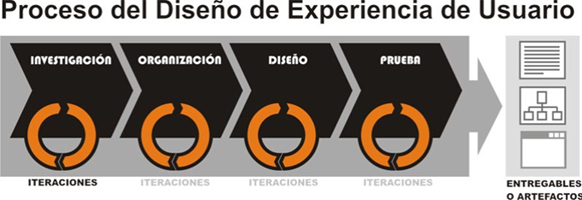
\includegraphics[width=0.5\linewidth]{figuras/proceso_diseno.png}
    \caption{Proceso de Diseño de Experencia de Usuario}
    \label{fig:enter-label}
\end{figure}


\section{Desarrollo Móvil en Android}
\subsection{Razones para elegir Android como plataforma de desarrollo}
Una de las razones principales para elegir Android como plataforma de desarrollo es su alta popularidad Guatemala. Según estudio la mayoría de celulares usados en el país son Samsung y Huawei, los cuales tienen sistema operativo Android \cite{Anonimo2019}.

Según datos recientes, Android domina el tráfico web móvil en el país, con un 82.50\% de participación. Esto significa que la mayoría de los usuarios de dispositivos móviles en Guatemala utilizan este sistema operativo, lo que amplía significativamente el alcance y la accesibilidad del producto desarrollado en esta plataforma \cite{Shum2023}.

\begin{figure} [h]
    \centering
    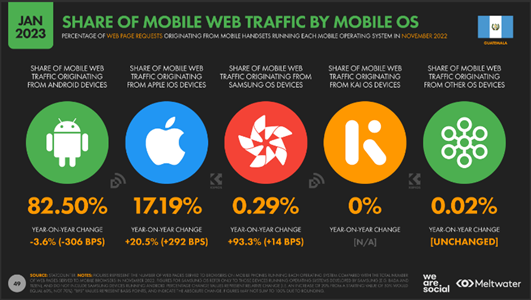
\includegraphics[width=0.5\linewidth]{figuras/mobile_web_traffic.png}
    \caption{Cuota de tráfico web móvil por sistema operativo}
    \label{fig:enter-label}
\end{figure}

Asimismo, Android es conocido por su diversidad en términos de dispositivos, desde teléfonos de alta gama hasta opciones más accesibles. También ofrece un alto nivel de flexibilidad y opciones de personalización, lo que facilita el desarrollo de aplicaciones. Finalmente, el ecosistema de desarrollo de Android está soportado con una vasta cantidad de recursos, herramientas y una comunidad activa de desarrolladores \cite{AnonimoAndroid}.

\subsection{Arquitectura de aplicaciones Android}
La arquitectura de una aplicación Android se basa en el patrón Modelo - Vista - Controlador (MVC). Aunque es muy común utilizar MVVM (Modelo - Vista - \textit{ViewModel}), pues ofrece una separación más clara de la lógica de presentación y facilita el mantenimiento en comparación con MVC \cite{RamosSF}.

\subsubsection{Componentes}
\begin{itemize}
    \item \textbf{Modelo}: Contiene los datos, el estado y la lógica del negocio \cite{Bhadoria2013}.
    \item \textbf{Vista}: Representa la interfaz de usuario. Se comunica con el \textit{ViewModel} a través de mecanismos de enlace de datos (\textit{data binding}), permitiendo una actualización automática de la UI cuando cambian los datos \cite{Bhadoria2013}.
    \item \textbf{\textit{ViewModel}}: Actúa como un intermediario entre el Modelo y la Vista. Expone datos y comandos que la Vista puede consumir y ejecutar, y notifica a la Vista sobre cambios en los datos utilizando observables (como \textit{LiveData}) \cite{Bhadoria2013}.
\end{itemize}

\subsubsection{Flujo de Trabajo}
\begin{itemize}
    \item La Vista se enlaza automáticamente al \textit{ViewModel} para observar los datos \cite{Bhadoria2013}.
    \item El \textit{ViewModel} obtiene los datos del Modelo y prepara la lógica de presentación \cite{Bhadoria2013}.
    \item Cualquier cambio en el Modelo se refleja automáticamente en la Vista a través del \textit{ViewModel} \cite{Bhadoria2013}.
    \item La interacción del usuario en la Vista invoca métodos en el \textit{ViewModel}, que a su vez pueden actualizar el Modelo \cite{Bhadoria2013}.
\end{itemize}

\begin{figure} [H]
    \centering
    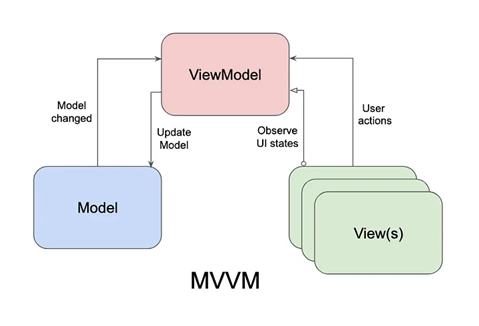
\includegraphics[width=0.5\linewidth]{figuras/mvvm.png}
    \caption{Diagrama de funcionamiento MVVM}
    \label{fig:enter-label}
\end{figure}

\subsection{Buenas prácticas de desarrollo Android}
Al desarrollar aplicaciones para Android, es esencial seguir ciertas buenas prácticas para asegurar la calidad y la eficiencia del producto final \cite{PhillipsStewart2022}:

\subsubsection{Uso de \textit{Layouts} Adecuados}
\begin{itemize}
    \item \textbf{\textit{ConstraintLayout}}: Es eficiente y flexible, permitiendo posicionar elementos de manera relativa a otros elementos \cite{PhillipsStewart2022}.
    \item \textbf{\textit{LinearLayout}}: Organiza los elementos en una sola fila o columna, siendo útil para diseños sencillos y alineaciones básicas \cite{PhillipsStewart2022}.
    \item \textbf{\textit{RelativeLayout}}: Permite posicionar los componentes en relación a otros o a sus propios padres, ofreciendo más flexibilidad pero con un mayor costo de rendimiento comparado con \textit{ConstraintLayout} \cite{PhillipsStewart2022}.
\end{itemize}

\subsubsection{Gestión de Recursos}
\begin{itemize}
    \item Utilizar unidades independientes de densidad (dp) para asegurar que los elementos de la interfaz mantengan su tamaño y proporciones adecuadas en dispositivos con diferentes tamaños de pantalla \cite{PhillipsStewart2022}.
    \item Definir colores, estilos y dimensiones en archivos de recursos para promover la reutilización y mantener la consistencia del diseño \cite{PhillipsStewart2022}.
    \item Utilizar \textit{Gradle} para gestionar dependencias, lo que te permitirá mantener el código actualizado y seguro \cite{PhillipsStewart2022}.
\end{itemize}

\subsubsection{Optimización del Rendimiento}
\begin{itemize}
    \item Minimizar el uso de vistas anidadas para mejorar el rendimiento de la interfaz de usuario \cite{PhillipsStewart2022}.
    \item Evitar operaciones pesadas en el hilo principal \cite{PhillipsStewart2022}.
\end{itemize}

\subsubsection{Seguridad}
\begin{itemize}
    \item Proteger los datos del usuario mediante el uso de almacenamiento cifrado y permisos adecuados \cite{PhillipsStewart2022}.
    \item Validar las entradas del usuario para prevenir ataques de inyección y otras vulnerabilidades de seguridad \cite{PhillipsStewart2022}.
    \item Validar permisos de uso de almacenamiento, cámara, micrófono, etc para respetar las políticas de privacidad de Android \cite{PhillipsStewart2022}.
\end{itemize}


	\fi
\fi


% METOLOGIA
% --------------------------------------------------------------------------------
\newpage
\thispagestyle{empty}
\mbox{}
\newpage 

\ifdefined\CAPmetodologia
	\newpage
	\chapter{Metodología}
	\ifdefined\parpordefecto
		\defaultparformat{metodologia}
	\else
		% MODULO DE DISEÑO =============

\section{INVESTIGACIÓN DE MERCADO}

\subsection{Investigación y revisión sobre aplicaciones y tecnologías similares}

Se investigan aplicaciones con funcionalidades parecidas a la solución propuesta por Señas Chapinas. 

\subsubsection{Hand Talk Translator}

Es una aplicación gratuita para dispositivos Android e iOS diseñada para mejorar la comunicación entre la comunidad sorda y las personas que pueden oír. Esta traduce texto, ya sea en texto o en audio, al lenguaje de señas americanas. Esto se realiza por medio de Hugo, un avatar tridimensional animado por IA, que facilita la traducción y el aprendizaje. Los usuarios tienen la opción de repetir las traducciones, modificar la velocidad de Hugo, guardar y calificar sus traducciones preferidas. También pueden crear mensajes en GIF para compartir y personalizar la apariencia de Hugo en su tienda \cite{Foggetti2023}.

    
\begin{itemize}
    \item \textbf{Funcionalidades destacadas}
    \begin{itemize}
        \item Traducción de frases a lengua de señas ASL mostrado a través de animación 3D.
        \item Opción de compartir por GIF en redes sociales.
        \item Opción de guardar traducción en favoritos.
        \item Opción de repetir la traducción y cambiar la velocidad de reproducción.
    \end{itemize}
    
    \item \textbf{Características de Diseño}
    \begin{itemize}
        \item Incorpora elementos interactivos y de personalización para mejorar la experiencia del usuario. Esto vuelve la aplicación más atractiva y personal.
        \item Animación fluida de Hugo, que facilita el seguimiento visual de las señas.
        \item Interfaz intuitiva y simple que permite una navegación sencilla por las distintas funciones de la aplicación.
        \item Uso de color naranja que induce calidez, alegría, optimismo y confianza.
        \item Los íconos y botones son grandes y están claramente etiquetados, lo cual es útil para una rápida identificación de la funcionalidad.
        \item La interfaz es responsiva.
    \end{itemize}

    \item \textbf{Comentarios de usuarios}
    \begin{itemize}
        \item Los usuarios solicitan que la aplicación traduzca palabras y no letra por letra.
        \item Los usuarios solicitan mayor cantidad de palabras disponibles para traducción a señas.
    \end{itemize}
\end{itemize}

\begin{figure} [h]
    \centering
    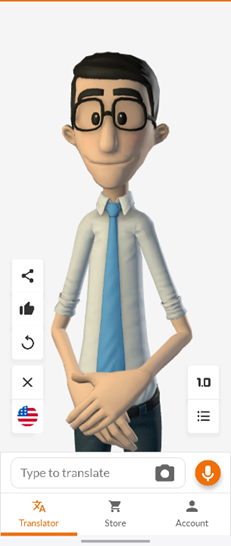
\includegraphics[width=0.25\linewidth]{figuras/handTalk.png}
    \caption{Muestra de aplicación “Hand Talk Translator”}
    \label{fig:enter-label}
\end{figure}


\subsubsection{SLAIT – Real-time Sign Language Translator with AI}

Es una aplicación en fase beta que ofrece servicios de traducción de lengua de señas americanas en tiempo real para dispositivos móviles, web, entre otros. Utiliza inteligencia artificial para realizar traducciones en tiempo real, otorgando facilidad de comunicación para comunicación diaria, salud, educación y oficina. Esta aplicación tendrá modalidad de pago, aunque permite ser parte de la aplicación beta sin costo pero con previo análisis del caso por la empresa \cite{SLAIT}.

\begin{itemize}
    \item \textbf{Funcionalidades destacadas}
    \begin{itemize}
        \item Traducción instantánea de voz a texto.
        \item Traducción instantánea de señas a texto.
    \end{itemize}

    \item \textbf{Características de Diseño}
    \begin{itemize}
        \item Diseño simple y amigable con el usuario.
    \end{itemize}
\end{itemize}

\begin{figure} [H]
    \centering
    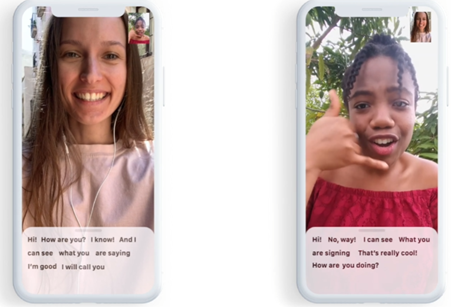
\includegraphics[width=0.5\linewidth]{figuras/slait.png}
    \caption{Muestra de aplicación “SLAIT”}
    \label{fig:enter-label}
\end{figure}

\subsubsection{Lenguaje de Señas IA}

La aplicación ofrece una plataforma de traducción de señas ASL a texto y viceversa, con múltiples funciones como búsqueda por categoría, emoji y alfabeto, y soporte para diez idiomas. Con más de 2,600 señas reconocidas, busca facilitar la comunicación y el aprendizaje del lenguaje de señas \cite{LenguajeDeSeñasIA}.

\begin{itemize}
    \item \textbf{Funcionalidades destacadas}
    \begin{itemize}
        \item Grabación de señas ASL para su reconocimiento y traducción a 10 diferentes idiomas.
        \item Traducción de frases en inglés a señas ASL, seña por seña.
        \item Búsqueda de señas por emoji, categoría, palabra y alfabéticamente.
    \end{itemize}

    \item \textbf{Características de Diseño}
    \begin{itemize}
        \item Paleta de colores e iconografía básica.
        \item Diseño confuso y apretado.
    \end{itemize}
\end{itemize}

\begin{figure}[H]
    \centering
    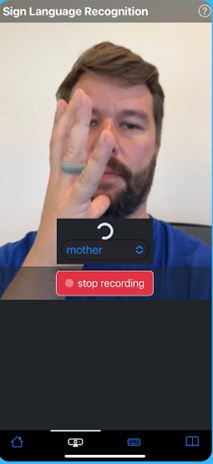
\includegraphics[width=0.2\linewidth]{figuras/applenguasenasia.png}
    \caption{Muestra de aplicación “Lenguaje de señas IA”}
    \label{fig:enter-label}
\end{figure}

\subsubsection{AI Sign: Sign Language}

Es una aplicación para IOS que utiliza inteligencia artificial para reconocer más de 100 señas americanas. Tiene dos modos: reconocimiento de acciones en tiempo real y captura de datos para mejorar la precisión del modelo de aprendizaje automático \cite{AISign2023}.

\begin{itemize}
    \item \textbf{Funcionalidades destacadas}
    \begin{itemize}
        \item Capacidad de reconocimiento en tiempo real.
        \item Contiene un modo de ayuda y ajustes de configuración para personalizar la experiencia.
    \end{itemize}

    \item \textbf{Características de diseño}
    \begin{itemize}
        \item Muestra de toma de datos de las señas, señalando puntos clave de la mano.
        \item No hay paleta de colores, se usan elementos gráficos básicos.
        \item Botones poco amigables y descriptivos.
    \end{itemize}
\end{itemize}


\begin{figure} [H]
    \centering
    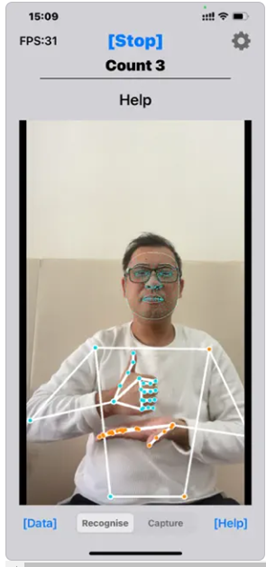
\includegraphics[width=0.25\linewidth]{figuras/ai_sign.png}
    \caption{Muestra de aplicación “AI Sign: Sign Language”}
    \label{fig:enter-label}
\end{figure}

\subsubsection{Sign Language Translator AI}

Es una aplicación móvil diseñada para reconocer y traducir el lenguaje de señas coreano. Utiliza inteligencia artificial para interpretar señas en tiempo real, buscando facilitar la comunicación para las personas sordomudas. La aplicación también fomenta la participación de los usuarios para mejorar su base de datos y aumentar la precisión del reconocimiento de gestos \cite{SignLanguageTranslatorAI}.

\begin{itemize}
    \item \textbf{Funcionalidades destacadas}
    \begin{itemize}
        \item Guías visuales para el posicionamiento correcto ante la cámara, esenciales para el reconocimiento de gestos.
        \item Capacidad de reconocimiento en tiempo real.
        \item Invitación a los usuarios para contribuir con sus propios gestos, ayudando a mejorar la base de datos.
        \item Lista de palabras reconocibles que sigue expandiéndose con las contribuciones de los usuarios.
    \end{itemize}

    \item \textbf{Características de diseño}
    \begin{itemize}
        \item Botones descriptivos.
        \item Interfaz simple y clara.
        \item Diseño intuitivo.
    \end{itemize}
\end{itemize}


\begin{figure} [H]
    \centering
    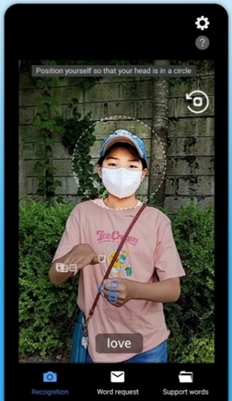
\includegraphics[width=0.25\linewidth]{figuras/ai_sign_lenguaje.png}
    \caption{Muestra de aplicación “Sign Language Translator AI”}
    \label{fig:enter-label}
\end{figure}

\subsubsection{Resumen de Funcionalidades y Características Destacadas de Aplicaciones Investigadas}

Luego de la investigación previa, se destacan las siguientes funcionalidades:
\begin{itemize}
    \item Espacio para grabar un video con indicadores de posición y luz adecuados para garantizar una captura óptima del vídeo.
    \item Modo ayuda para tutorial.
    \item Botón de compartir para difundir textos traducidos en redes sociales.
    \item Botón de agregar a favoritos la traducción realizada.
    \item Botón de reproducción de voz.
    \item Botón para calificar la traducción.
    \item Historial de videos grabados.
    \item Lista de palabras reconocibles.
\end{itemize}

Asimismo, destacan las siguientes características de diseño:
\begin{itemize}
    \item Diseño limpio e intuitivo.
    \item Paleta de colores atractiva.
    \item Botones descriptivos para mayor comprensión de su función.
\end{itemize}

% ---------------------------------------------------------------------------------------------------------------

\subsection{Investigación de la situación actual de los sordos en Guatemala}

En Guatemala, se estima que hay aproximadamente 240,000 personas sordas, lo que representa el 3\% de la población mayor de cuatro años, según datos del Instituto Nacional de Estadística (INE). Las causas de la sordera son diversas e incluyen factores genéticos, complicaciones durante el nacimiento y enfermedades infecciosas. Uno de los principales desafíos que enfrentan las personas sordas en el país es la comunicación, lo cual limita su capacidad para participar de manera equitativa en la sociedad \cite{CongresoGuatemala} \cite{GobiernoGuatemala2022}.

La lengua de señas reconocida es LENSEGUA. Las personas sordas están dispersas por todo el territorio nacional, pero se estima que la mayoría que saben LENSEGUA están concentradas principalmente en la ciudad capital. En áreas rurales con acceso limitado a la educación, como el norte de Petén, las personas sordas a menudo desarrollan sus propios sistemas de señas \cite{JoshuaProject}. 

El ámbito educativo presenta desafíos notables. A pesar de la existencia de organizaciones como la Asociación Nacional de Sordos de Guatemala, que brinda educación y otros servicios, las oportunidades educativas son escasas, especialmente en áreas rurales. Muchos estudiantes sordos deben alejarse de sus familias para acceder a opciones educativas que incluyan instrucción en lengua de señas. Un gran número de ellos ni siquiera tiene la oportunidad de acceder a una educación básica debido a la escasez de maestros capacitados en lengua de señas. Menos del 50\% recibe educación formal y las escuelas rara vez ofrecen niveles de educación secundaria. Aquellos que persiguen estudios superiores a menudo lo hacen sin la ayuda de intérpretes, lo que complica su aprendizaje y progreso académico. Esto perpetúa un ciclo de desventajas educativas y económicas, con altas tasas de desempleo y dependencia económica entre la comunidad sorda \cite{EndangeredLanguages}.

El desempleo es elevado en esta comunidad debido a las barreras comunicativas y la falta de adaptaciones adecuadas en los lugares de trabajo. La mayoría de las personas sordas vive con sus padres y están relegadas a trabajos de mano de obra básica debido a las barreras para obtener empleos mejor remunerados \cite{EndangeredLanguages}.

A pesar de estos retos, ha habido iniciativas para mejorar la inclusión de las personas sordas en Guatemala. Por ejemplo, el Benemérito Comité Pro-Ciegos y Sordos de Guatemala, en colaboración con SEGEPLAN, ha trabajado en promover la educación inclusiva y el empleo equitativo, aunque la implementación efectiva de estas políticas aún enfrenta obstáculos significativos \cite{GobiernoGuatemala2022}.

%------------------------------------------------------------------------------------------------------

\subsection{Preparación y realización de entrevistas y encuestas}

\subsubsection{Entrevista a Doctor Miguel Angel Gonzalez Palacios}

El Dr. Gonzalez, médico general con más de 25 años de experiencia, compartió sus reflexiones sobre la importancia de mejorar la comunicación con pacientes sordos. Durante la entrevista, destacó las dificultades que enfrenta en su práctica diaria, particularmente en la correcta comprensión de los síntomas y necesidades de los pacientes sordos, lo cual es fundamental para proporcionar un diagnóstico preciso y un tratamiento efectivo.

El Dr. Gonzalez expresó su entusiasmo por la iniciativa de la aplicación "Señas Chapinas", mencionando que una herramienta de este tipo podría ser revolucionaria para la práctica médica. Resaltó el potencial de la aplicación para facilitar una comunicación fluida y precisa con pacientes sordos, reduciendo los malentendidos y aumentando la calidad del cuidado médico. 

\subsubsection{Entrevista a Licenciada Claudia Barrillas}

En la entrevista con la abogada Barrillas, se abordó el contexto legal de las personas sordomudas en Guatemala, destacando la importancia de proteger sus derechos en los procedimientos judiciales. Se resaltó la necesidad de contar siempre con un intérprete de lengua de señas durante las declaraciones para asegurar una comunicación efectiva. La escasez de intérpretes, sin embargo, puede provocar demoras en los procesos legales. La Licenciada Barrillas enfatizó el valor de una aplicación de traducción de lengua de señas que podría permitir una comunicación más fluida y directa, reduciendo la dependencia de intermediarios y mejorando el acceso a la justicia para las personas sordomudas, fomentando la inclusión y la igualdad.

Se mencionaron casos donde la ausencia de intérpretes resultó en injusticias o malentendidos legales, subrayando la importancia de una comunicación clara y efectiva en el ámbito judicial. La profesional propuso que una aplicación de traducción de lengua de señas no solo facilitaría la comunicación en procesos legales, sino que también promovería una mayor autonomía para las personas sordomudas, eliminando muchas barreras que enfrentan cotidianamente.

\subsubsection{Entrevista con Profesora Carmen Lucía Guerrero}

Carmen Guerrero es profesora en la Universidad del Valle de Guatemala y forma parte del departamento de Educación para personas con necesidades especiales. Su trabajo le ha permitido adquirir conocimientos en LENSEGUA y establecer contacto directo con miembros de la comunidad sorda.

En esta entrevista se abordaron temas clave sobre la estructura y adaptación del español signado en la lengua de señas. 

La profesora Guerrero explicó que las personas que nacen sordas generalmente aprenden la lengua de señas como su primer idioma, lo cual posee una gramática y estructura propias, distintas del español hablado. Por otro lado, aquellas que pierden la audición más tarde en la vida pueden intentar adaptar su forma de hablar al español, conservando características del lenguaje oral. Este contraste muestra cómo la forma de comunicación varía significativamente entre quienes han sido sordos desde el nacimiento y quienes se han vuelto sordos posteriormente.

Uno de los desafíos discutidos fue la falta de un estándar unificado en la lengua de señas en Guatemala, lo que lleva al uso de señas específicas en regiones como Quetzaltenango. Esta variabilidad regional complica la comunicación y la educación en lengua de señas. Además, la profesora subrayó la importancia de contar con intérpretes y educadores certificados por el Ministerio de Educación para asegurar utilizar LENSEGUA “oficial”. 

También se mencionó que muchas de las señas utilizadas en Guatemala son adaptaciones de la lengua francesa, compartiendo similitudes gramaticales con este idioma. La licenciada recomendó la necesidad de investigar más sobre estas reglas gramaticales y consultar documentación específica que pueda profundizar el entendimiento y la correcta aplicación de la lengua de señas.

La conversación también resaltó la relevancia de la posición y el movimiento de las manos en la comunicación a través de señas, dado que pequeñas variaciones pueden alterar significativamente el significado de las palabras. Por ejemplo, las señas para ``hola'' y ``gracias'' son muy parecidas y pueden confundirse fácilmente. 

Finalmente, se recalcó que no siempre es posible traducir todas las palabras directamente a señas, lo que destaca la complejidad de desarrollar recursos efectivos para la comunicación en lengua de señas y la importancia de adaptar continuamente las herramientas educativas y de comunicación para satisfacer las necesidades de la comunidad sorda.


\subsubsection{Entrevista a intérprete de En-Señas Melany Cordero}

Melany Cordero, quien ejerce como intérprete y maestra de nivel medio en En-Señas, acompaña a profesoras al impartir clases y asiste en la resolución de dudas de los alumnos. Comenzó su formación en LENSEGUA en la academia y obtuvo su diploma que la acredita como intérprete.

Durante la entrevista, Melany expresó que la propuesta de la aplicación ``Señas Chapinas'' le pareció tanto útil como innovadora. Sugirió agregar elementos como juegos o retos diarios, para fomentar un aprendizaje continuo y efectivo de LENSEGUA entre los usuarios. Propuso, por ejemplo, implementar un juego de memoria o un ejercicio similar a los utilizados en exámenes, donde se presenta una palabra y los usuarios deben seleccionar la seña correcta asociada. Estas actividades no solo mantendrían el interés de los usuarios, sino que también potenciarían su capacidad de aprendizaje y retención de la lengua de señas de manera divertida y desafiante.


\subsubsection{Entrevista a Director General de En-Señas Antonio Barrientos}

El señor Barrientos desarrolló un interés por la lengua de señas inspirado por su madre, quien también la aprendió y frecuentaba a la comunidad sorda. Motivado por su deseo de entender las conversaciones de este grupo, el señor se sumergió en el estudio de la lengua de señas y actualmente es intérprete de nivel avanzado y director general de la institución ``En-Señas''.

Durante la entrevista, el Director señaló que una de las principales complicaciones con la aplicación ``Señas Chapinas'' es la falta de un estándar uniforme para LENSEGUA. Explicó que existen variaciones significativas en el uso de señas entre los diferentes departamentos de Guatemala, e incluso entre distintas instituciones educativas, lo que puede complicar la precisión de las traducciones. Esta diversidad se debe a la ausencia de una entidad reguladora que estandarice las señas y certifique quiénes están calificados para enseñar LENSEGUA. No obstante, actualmente hay esfuerzos para lograr esta estandarización.

El Director también destacó la escasez de materiales e información en línea sobre LENSEGUA, así como las deficiencias legislativas que, aunque reconocen la lengua de señas, no establecen un marco regulatorio suficiente para su enseñanza y promoción.

En cuanto a la comunidad sorda, mencionó que existen cuatro categorías distintas: personas que utilizan señas caseras y no interactúan con LENSEGUA, aquellas que aprenden a leer los labios, los usuarios de LENSEGUA, y los bilingües, que combinan la lectura de labios con el uso de la lengua de señas.

Finalmente, el Director Barrientos abordó el alto índice de analfabetismo en la comunidad sorda, atribuyéndolo a las diferencias en el nivel de apoyo que reciben desde la infancia. Mientras algunas familias fomentan el aprendizaje de la lengua de señas y la terapia del habla desde temprana edad, otras dejan a las personas sordas sin el soporte necesario para su desarrollo educativo.

\subsubsection{Entrevista a persona sorda hipoacúsica y maestra de En-Señas Gabriela Velázquez}
La señora Velázquez, una maestra de 59 años de En-Señas y persona sorda hipoacúsica, nació en Guatemala y actualmente enseña LENSEGUA tanto a personas sordas como oyentes. Está casada con una persona sorda profunda. 

Durante su infancia, la señora Gabriela relata que era común que las personas sordas fueran obligadas a aprender a vocalizar mediante terapia del habla y lectura de labios, en lugar de aprender LENSEGUA. No fue hasta la edad adulta que aprendió este medio de comuniación, convirtiéndose en bilingüe, lo cual marcó una mejora significativa en su comprensión lectora y en la ampliación de su vocabulario. Aunque la profesora puede leer labios, encuentra este método desafiante y prefiere comunicarse usando LENSEGUA, lo que le resulta más cómodo y eficaz. Ella señala que, para las personas sordas profundas, vocalizar puede ser aún más difícil, por lo que generalmente dependen más de LENSEGUA, lo que a menudo complica su comprensión del español escrito.

Sobre la aplicación ``Señas Chapinas'', la profesora Gabriela considera que sería útil para usuarios de LENSEGUA y destacó la importancia de que la aplicación ofrezca tanto la traducción palabra por palabra como la oración completa en español. Esto ayudaría a los usuarios a verificar la traducción de las señas y facilitaría el aprendizaje de la gramática en español. La profesora Velázquez y sus conocidos frecuentemente utilizan \textit{ChatGPT}, escribiendo en gramática de LENSEGUA para que el sistema lo traduzca al español, lo que les ayuda a confirmar que están escribiendo correctamente.

Ella menciona que ``Señas Chapinas'' la usaría principalmente en situaciones donde no hay un intérprete presente, como visitas al médico, reuniones con abogados, testimonios en corte, emergencias y reuniones familiares. Menciona que en Estados Unidos existe un servicio de intérpretes que funciona como un \textit{call center}, donde se ofrece traducción a lengua de señas de forma simultanea, y sugiere que la aplicación podría replicar este servicio en Guatemala, ofreciendo traducciones de LENSEGUA a texto o voz.

Además, destacó que la aplicación podría contribuir a reducir el analfabetismo entre los sordos, permitiéndoles aprender al grabar videos en LENSEGUA y ver las traducciones al español. 

En el contexto de las aplicaciones móviles, se destacó que las personas sordas utilizan continuamente sus teléfonos, especialmente para acceder a redes sociales y aplicaciones de videollamadas. Estas herramientas les permiten interactuar con amigos, familiares y conocidos de manera más dinámica. Continua relatando que antes de la llegada de los teléfonos inteligentes, la comunicación era notablemente más complicada; sin embargo, hoy en día, la tecnología facilita significativamente el aprendizaje de LENSEGUA en línea y mejora la comunicación general. 

La profesora Velázquez prefiere las aplicaciones que requieren poco texto y presentan interfaces de usuario simples y directas, ya que son más fáciles de utilizar. Además, comentó que las aplicaciones lentas y complejas resultan menos atractivas para los ella y sus conocidos.

Para la profesora, un aspecto crucial de la aplicación ``Señas Chapinas'' es que reconozca las diversas variantes y modismos presentes en LENSEGUA. Este detalle es fundamental para asegurar que la aplicación sea verdaderamente inclusiva y efectiva para todos los usuarios de la lengua de señas guatemalteca, reflejando las diferencias regionales y de estilo que caracterizan su uso cotidiano.

Además, Gabriela Velázquez espera que la aplicación le sirva como una herramienta para enriquecer su vocabulario y gramática en español. Al incorporar funciones que permitan aprender y practicar español, la aplicación no solo serviría para traducir de LENSEGUA a español, sino que también funcionaría como un recurso educativo, apoyando el desarrollo lingüístico integral de sus usuarios.


\begin{figure} [H]
    \centering
    \includegraphics[width=0.5\linewidth]{figuras/entrevista.png}
    \caption{Entrevista En-Señas}
    \label{fig:enter-label}
\end{figure}

\subsubsection{Primera encuesta Señas Chapinas}

La primera encuesta para el proyecto ``Señas Chapinas'' consta de varias secciones diseñadas para recopilar información y opiniones sobre la necesidad de superar las barreras de comunicación en Guatemala a través de una aplicación móvil.

La primera sección recopila datos demográficos como edad, género, lugar de nacimiento, profesión y si el encuestado presenta dificultades auditivas o del habla.

La segunda sección está bifurcada según si los encuestados son sordos o no. Para los que no son sordos, se investiga si conocen a alguien con dificultades auditivas y cómo han utilizado tecnología de asistencia para comunicarse con ellos. Además, se indaga sobre los desafíos percibidos para estas personas y en qué contextos una aplicación de traducción de señas sería beneficiosa. Para los encuestados sordos, se solicita que compartan sus experiencias con otras herramientas de asistencia, desafíos específicos enfrentados en Guatemala, situaciones de frustración al comunicarse, y cómo una aplicación podría mejorar su comunicación diaria.

La tercera sección evalúa la percepción sobre la utilidad de la aplicación para convertir la lengua de señas a texto o voz, recogiendo expectativas y características deseadas. Además, se piden sugerencias sobre funcionalidades adicionales y posibles contextos de uso.

Los resultados de esta primera encuesta no fueron los esperados. Los participantes sordos de nacimiento encontraron las preguntas demasiado complejas, atribuyéndolo a las diferencias gramaticales en su lenguaje. Esto llevó a la necesidad de desarrollar una encuesta específica para personas oyentes y planificar entrevistas con intérpretes para personas sordas.


\subsubsection{Segunda encuesta Señas Chapinas}

Como resultado de los comentarios y sugerencias recopilados en la primera encuesta, se desarrolló una segunda encuesta dirigida específicamente a personas oyentes (ver Anexo~\ref{anexo:encuesta_oyentes}). Esta encuesta se dirige a individuos sin conocimiento previo de LENSEGUA, a aquellos que regularmente interactúan con personas sordas, y a intérpretes. 

La sección inicial de la encuesta proporciona un análisis demográfico de los participantes. Los resultados muestran que la mayoría de los encuestados son hombres. Además, el grupo de edad más representado está entre los 18 y 24 años. 

\begin{figure} [H]
    \centering
    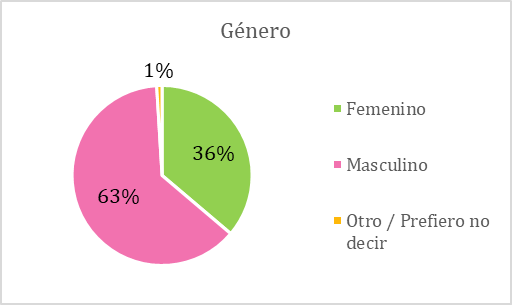
\includegraphics[width=0.5\linewidth]{figuras/encuesta_genero.png}
    \caption{Género Encuesta 2}
    \label{fig:enter-label}
\end{figure}

\begin{figure} [H]
    \centering
    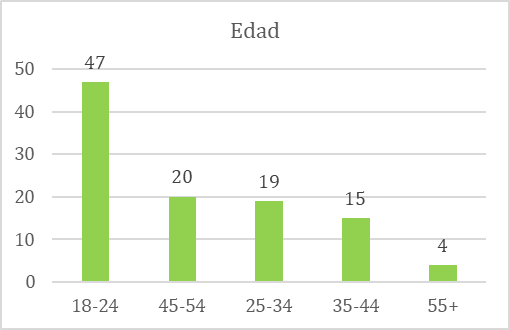
\includegraphics[width=0.5\linewidth]{figuras/encuesta_edad.png}
    \caption{Edad Encuesta 2}
    \label{fig:enter-label}
\end{figure}

La siguiente sección de la encuesta está destinada a explorar el conocimiento y la experiencia con la lengua de señas. Alrededor del 40\% de los encuestados indica conocer a alguien sordo, lo que destaca una conexión significativa con la comunidad sorda. Adicionalmente, cerca del 70\% percibe la aplicación como relevante, mostrando un interés considerable en la herramienta propuesta. Sin embargo, es notable que aproximadamente el 70\% de los participantes no están familiarizados con LENSEGUA, lo cual es entendible considerando que su reconocimiento oficial data de hace solo cuatro años. \cite{CongresoGuatemala2020}. 

\begin{figure} [H]
    \centering
    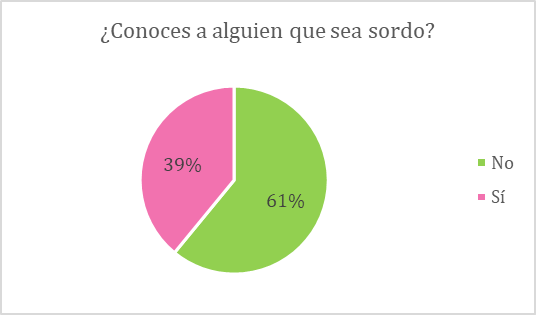
\includegraphics[width=0.5\linewidth]{figuras/conocimientoSordaEncuesta.png}
    \caption{Conocimiento Persona Sorda Encuesta 2}
    \label{fig:enter-label}
\end{figure}

\begin{figure} [H]
    \centering
    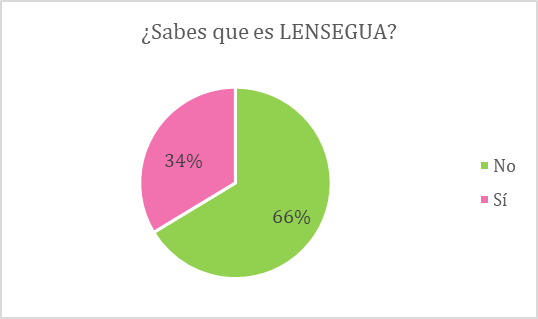
\includegraphics[width=0.5\linewidth]
    {figuras/conoimiento_lensegua.png}
    \caption{Conocimiento LENSEGUA Encuesta 2}

\end{figure}

\begin{figure} [H]
    \centering
    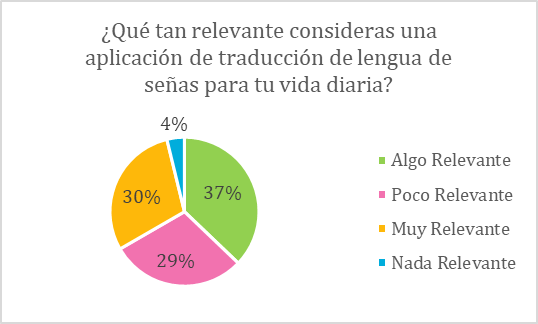
\includegraphics[width=0.5\linewidth]{figuras/relevancia_app.png}
    \caption{ Relevancia de la Aplicación Encuesta 2}
    \label{fig:enter-label}
\end{figure}


Además, se realizó un análisis comparativo entre los encuestados que conocen a personas sordas y su percepción de la relevancia de la aplicación. Los resultados muestran que aquellos familiarizados con la comunidad sorda tienden a valorar más la aplicación en comparación con quienes no tienen contacto directo con personas sordas. Este hallazgo sugiere que la experiencia personal y el conocimiento de los retos enfrentados por las personas sordas pueden influir significativamente en la percepción de la utilidad de herramientas tecnológicas como un traductor de lengua de señas.

\begin{figure} [H]
    \centering
    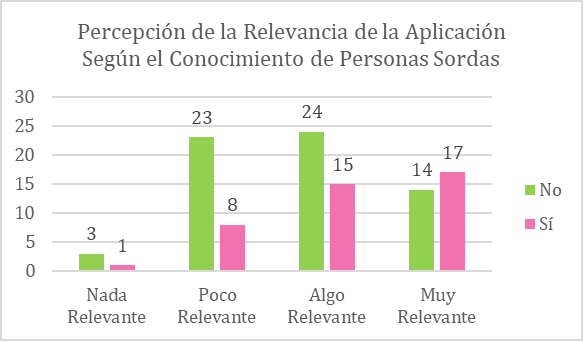
\includegraphics[width=0.5\linewidth]{figuras/relevancia_app_conocidos.png}
    \caption{Relevancia de la Aplicación para Personas con Conocidos Sordos Encuesta 2}
    \label{fig:enter-label}
\end{figure}

Para comprender mejor las estrategias de comunicación que las personas emplearían con individuos sordos, se les preguntó a los encuestados sobre sus métodos preferidos. La mayoría, casi el 60\%, optaría por el uso de mensajes escritos, mientras que un 18\% indicó que señalarían objetos para hacerse entender. Solo un 9\% consideraría usar LENSEGUA. Es notable que solo una minoría, aproximadamente el 10\%, expresó no saber cómo comunicarse, reflejando así el interés general por explorar formas de interacción. Algunos participantes también mencionaron la lectura de labios como alternativa, aunque es importante destacar que no todos los sordos tienen la capacidad de leer los labios.

Para profundizar en el entendimiento que tienen las personas sobre los desafíos que enfrentan los sordos, se les preguntó cuáles consideraban que eran las mayores dificultades para esta comunidad. Las respuestas revelaron una conciencia sobre la falta de inclusión y herramientas adecuadas para personas sordas, destacando cómo muchas infraestructuras y servicios en Guatemala están diseñados principalmente para oyentes. Además, se mencionaron problemas como segregación y discriminación en la sociedad, así como la escasez de enseñanza de la lengua de señas.

Entre las preocupaciones más citadas también estuvieron la ausencia de sistemas de alerta para sordos en situaciones de emergencia y barreras significativas en comunicación. Los encuestados resaltaron la existencia de prejuicios y la dificultad en la realización de tareas cotidianas y trámites, lo que contribuye al aislamiento social y a la exclusión. Esta variedad de respuestas ilustra la complejidad de los desafíos a los que se enfrentan los sordos. 

La siguiente sección de la encuesta se centró en la aplicación "Señas Chapinas", explorando las motivaciones principales para usar una herramienta de traducción de lengua de señas. Destacablemente, el 60\% de los participantes indicaron la curiosidad personal como su principal motivación. Casi la mitad de los encuestados mencionaron la comunicación con amigos o familiares sordos como un factor importante, subrayando la relevancia personal y social de la aplicación. Además, cerca del 40\% expresaron que utilizarían la aplicación para actividades voluntarias, lo que refleja su potencial utilidad en entornos de servicio comunitario. Un pequeño porcentaje citó los requerimientos laborales como motivo, sugiriendo su aplicación en contextos profesionales donde la interacción con personas sordas es frecuente. Otras respuestas revelaron usos más específicos y personales, evidenciando la diversidad de situaciones en las que los usuarios anticipan la utilidad de la aplicación.

También se indagó en que situaciones los usuarios desean emplear la aplicación ``Señas Chapinas''. Predominantemente, las actividades sociales representan el escenario más popular, con un 78.6\% de los encuestados seleccionándolo. Esto es seguido por el voluntariado y la educación, con un 67.6\% y un 49\%, respectivamente. El trabajo también es una situación comúnmente identificada, con un 40.2\% de los encuestados expresando la necesidad de utilizar la aplicación en este contexto. Estos resultados indican una fuerte preferencia por utilizar la aplicación en contextos grupales y de interacción, lo que subraya la importancia de la aplicación en facilitar la comunicación en una variedad de entornos cotidianos y profesionales.

La última sección pregunta las características más importantes en una aplicación móvil. En la última sección de la encuesta, los encuestados identificaron las características más importantes en una aplicación móvil. La facilidad de uso fue la más destacada, valorada por el 98.1\% de los participantes, seguida por la velocidad y rendimiento (61.9\%), funciones de accesibilidad (54.3\%), y diseño atractivo (46.7\%). Esto resalta la importancia de una interfaz intuitiva, un rendimiento eficiente, accesibilidad adecuada, y un diseño visualmente atractivo para los usuarios de esta aplicación. 

Finalmente se dio espacio para comentarios adicionales. En la sección final de la encuesta se exploraron las características esenciales para una aplicación de traducción de lengua de señas. La facilidad de uso fue una de las características más mencionadas, destacando su importancia para una adopción rápida por parte de los usuarios. Muchos encuestados valoraron también la velocidad y la precisión de la traducción, subrayando la necesidad de interacciones fluidas y sin errores. Algunas otras sugerencias fueron mencionadas, pero serán tomadas en cuenta para futuras mejoras, pues no están dentro del alcance del presente proyecto. 

\subsubsection{Entrevista Colectiva a miembros de En-Señas}

Con un conocimiento más profundo de las necesidades de las personas sordas, sus familias y conocidos, así como del nivel de conciencia de la población guatemalteca sobre LENSEGUA, se llevó a cabo una última entrevista colectiva con miembros de Enseñas. Durante esta sesión, se presentó el concepto de la aplicación y se recogieron sus opiniones. Los comentarios más destacados incluyeron:

\begin{itemize}
    \item \textbf{Uso de Redes Sociales:} Las personas sordas frecuentan plataformas sociales, especialmente TikTok, por su facilidad e intuitividad de uso.
    
    \item \textbf{Funcionalidades Educativas}: Se sugirió que la aplicación también debería facilitar el aprendizaje de LENSEGUA en Guatemala, incorporando juegos interactivos que fomenten la participación activa.
    
    \item \textbf{Diseño Atractivo y Profesional}: La aplicación debe ser visualmente llamativa sin sacrificar su seriedad, generando confianza en que se trata de una herramienta fiable y efectiva.
    
    \item \textbf{Futuras Expansiones}: Se anticipa que, eventualmente, la aplicación podrá traducir del español a LENSEGUA.
    
    \item \textbf{Vocabulario Adecuado}: En las primeras fases, el vocabulario debe ser simple y cotidiano, incluyendo términos de uso frecuente y frases de emergencia.
    
    \item \textbf{Reporte de Errores:} Es crucial que las traducciones incorrectas puedan ser reportadas fácilmente por los usuarios sordos para que el equipo detrás de la aplicación pueda investigar y resolver cualquier inconveniente.
    
    \item \textbf{Guardado de Favoritos:} Los usuarios expresaron el deseo de poder guardar videos de frases en LENSEGUA que utilizan regularmente, para acceder a ellos de manera rápida y sencilla.
    
    \item \textbf{Flexibilidad de Grabación}: La aplicación debe permitir grabaciones tanto con la cámara frontal como con la trasera, facilitando la captura de auto-grabaciones o de terceros.
    
    \item \textbf{Accesibilidad del Nombre}: El nombre de la aplicación debe ser fácilmente representable en señas, asegurando su accesibilidad y reconocimiento dentro de la comunidad sorda.
    
\end{itemize}

Estos valiosos comentarios guiaran la próxima fase de desarrollo para asegurar que la aplicación no solo cumpla con las expectativas de la comunidad sorda sino que también sirva como un puente cultural y educativo.


\begin{figure} [H]
    \centering
    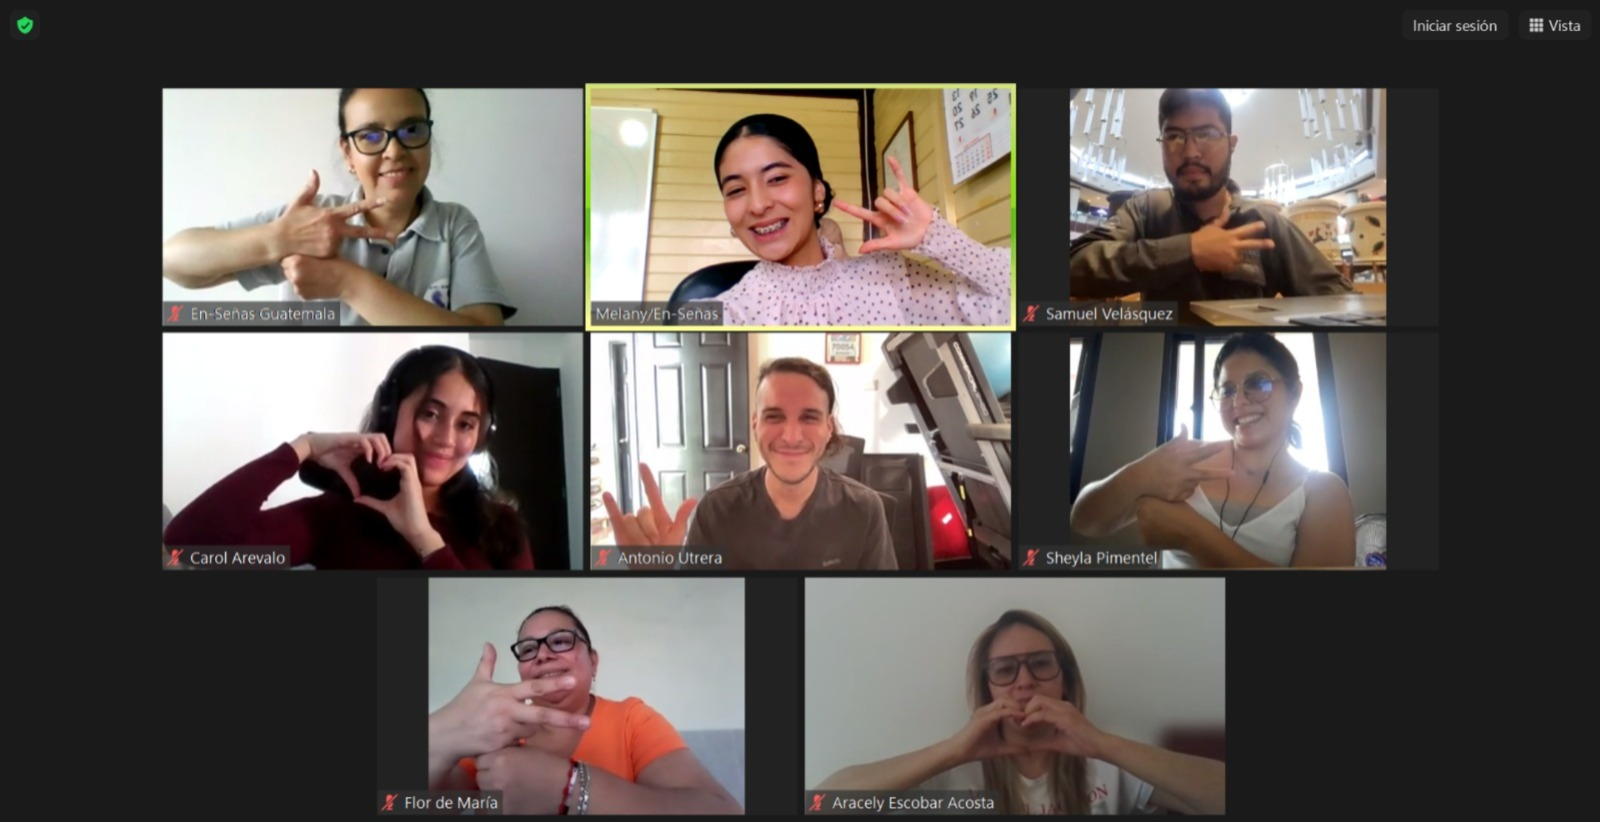
\includegraphics[width=0.75\linewidth]{figuras/entrevista_colectiva.png}
    \caption{Entrevista colectiva En-Señas}
    \label{fig:enter-label}
\end{figure}


%-------------------------------------------------------------------------------------------------------------------------------

\subsection{Colaboraciones}

Para profundizar en la comprensión de las necesidades tanto de las personas sordas como de aquellas que desean comunicarse con ellas, se decidió colaborar con varias entidades guatemaltecas dedicadas a mejorar la calidad de vida de este grupo.

En primer lugar, se participó en clases de Lengua de Señas Guatemalteca (LENSEGUA) ofrecidas por En-Señas. Esta formación permitió comprender mejor la gramática y el contexto cultural de esta lengua, elementos fundamentales para garantizar una comunicación efectiva y respetuosa.

Asimismo, la empresa ASEDES colaboró proporcionando apoyo en la realización de entrevistas y en otras actividades necesarias para el desarrollo de los diversos módulos del proyecto. Esta colaboración fue vital para asegurar que el diseño de la aplicación sea inclusivo y práctico para los usuarios.

Finalmente, la ONG Sordos Latinos de Guatemala estuvo brindando asistencia invaluable mediante el suministro de información y recomendaciones especializadas. Además, facilito entrevistas y otros recursos esenciales que enriquecieron el entendimiento y ayudaron a ajustar el proyecto para entender mejor las necesidades de la comunidad sorda en Guatemala.

%======================================================================================================
\section{DESARROLLO DE INTERFAZ Y EXPERIENCIA DE USUARIO}

\subsection{Creación de Diagrama de Afinidad}

En el desarrollo de la experiencia del usuario (UX), los diagramas de afinidad juegan un papel crucial, ya que permiten organizar y sintetizar grandes volúmenes de datos e ideas de manera visual y estructurada. Este método es especialmente valioso durante las fases iniciales de desarrollo de un proyecto, donde el entendimiento claro y la definición del problema son esenciales \cite{Maze2024}.

El proceso comienza con una lluvia de ideas, donde se generan y recopilan múltiples puntos de vista y datos sobre las necesidades y problemas de los usuarios. Esta fase es crítica, ya que establece la base de información que influirá en todas las decisiones de diseño y desarrollo subsiguientes \cite{Maze2024}.

La lluvia de ideas para Señas Chapinas organiza conceptos clave en categorías codificadas por colores, facilitando la identificación y el análisis de diversas áreas del proyecto:

\begin{itemize}
    \item \textbf{Naranja:} Define el público objetivo de la aplicación.
    \item \textbf{Amarillo:} Enumera los objetivos y metas que la aplicación pretende alcanzar.
    \item \textbf{Azul:} Destaca información crucial necesaria para el desarrollo de la aplicación.
    \item \textbf{Rojo:} Señala los problemas y desafíos que la aplicación busca resolver.
    \item \textbf{Verde:} Detalla las características y funcionalidades esperadas de la aplicación.
\end{itemize}

Este enfoque visual no solo ayuda a estructurar el proceso de planificación, sino que también asegura que todos los aspectos relevantes sean considerados, apoyando una toma de decisiones informada y alineada con las necesidades de los usuarios.

\begin{figure} [H]
    \centering
    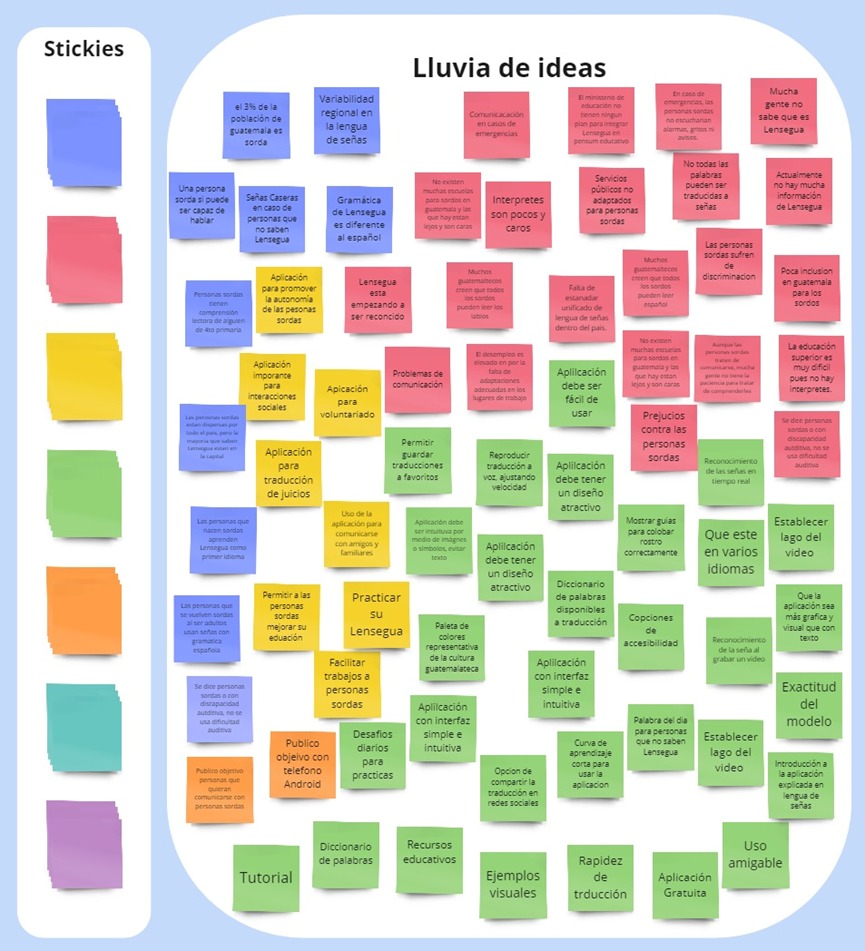
\includegraphics[width=0.75\linewidth]{figuras/lluevia_diagrama_afinidad.png}
    \caption{Lluvia de Ideas para Diagrama de Afinidad}
    \label{fig:enter-label}
\end{figure}

Posteriormente, se agrupan las ideas similares con el objetivo de identificar patrones y temas comunes. Este proceso implica organizar los datos recolectados durante la lluvia de ideas en categorías que reflejen conexiones y tendencias subyacentes. Al hacer esto, se pueden observar relaciones entre las diferentes opiniones y necesidades, facilitando la creación de soluciones más coherentes y efectivas que aborden los desafíos identificados de manera integral. Este método no solo ayuda a clarificar el alcance del proyecto, sino que también proporciona una base sólida para las decisiones de diseño y desarrollo subsiguientes, asegurando que se consideren todas las perspectivas relevantes.

\begin{figure} [H]
    \centering
    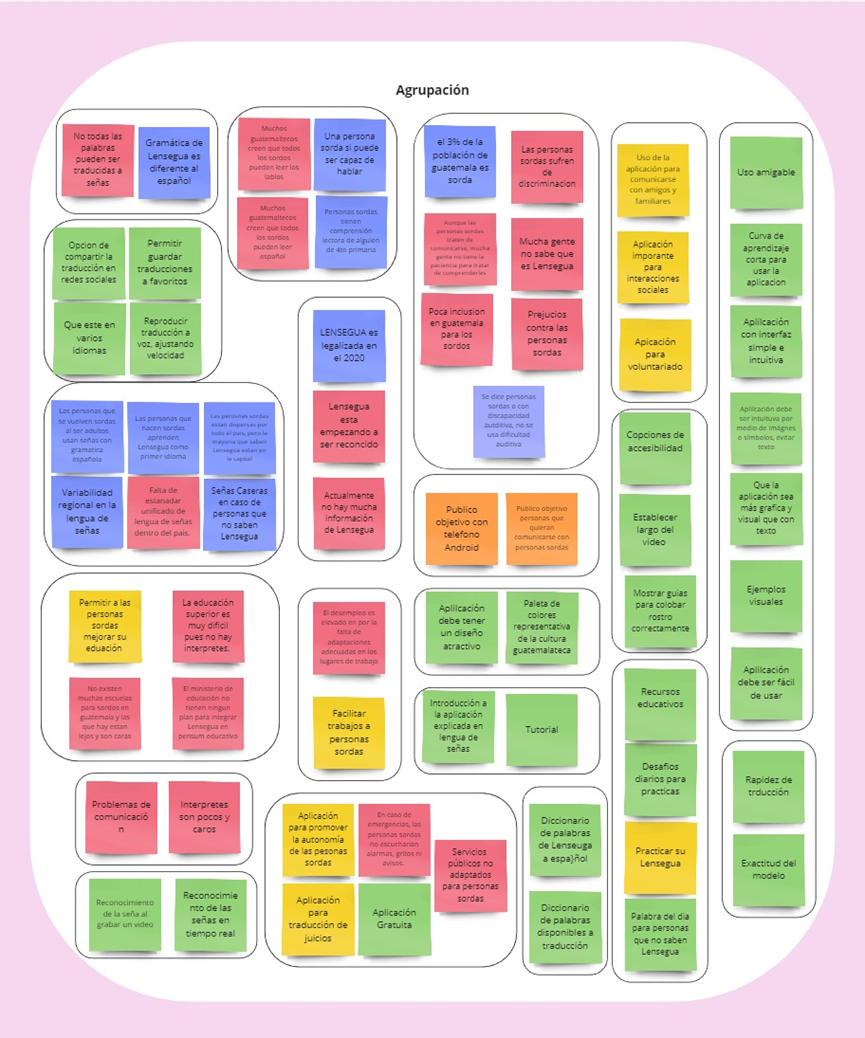
\includegraphics[width=0.75\linewidth]{figuras/agrupacion_diagrama_afinidad.png}
    \caption{Agrupación de Ideas para Diagrama de Afinidad}
    \label{fig:enter-label}
\end{figure}

Finalmente, se realiza el diagrama de afinidad, que sintetiza todas las ideas recolectadas y categorizadas previamente. Este diagrama visual, organizado por colores, facilita la interpretación de la información y permite una evaluación clara de cómo cada aspecto del proyecto interacciona y contribuye al objetivo global. Al agrupar las ideas en distintas categorías, como Público Objetivo, Problemas a Resolver, Objetivos, Escenarios de Uso, Funcionalidades a Desarrollar y Características de la Aplicación, se destaca la interconexión entre los requisitos del usuario y las soluciones propuestas.

\begin{figure} [H]
    \centering
    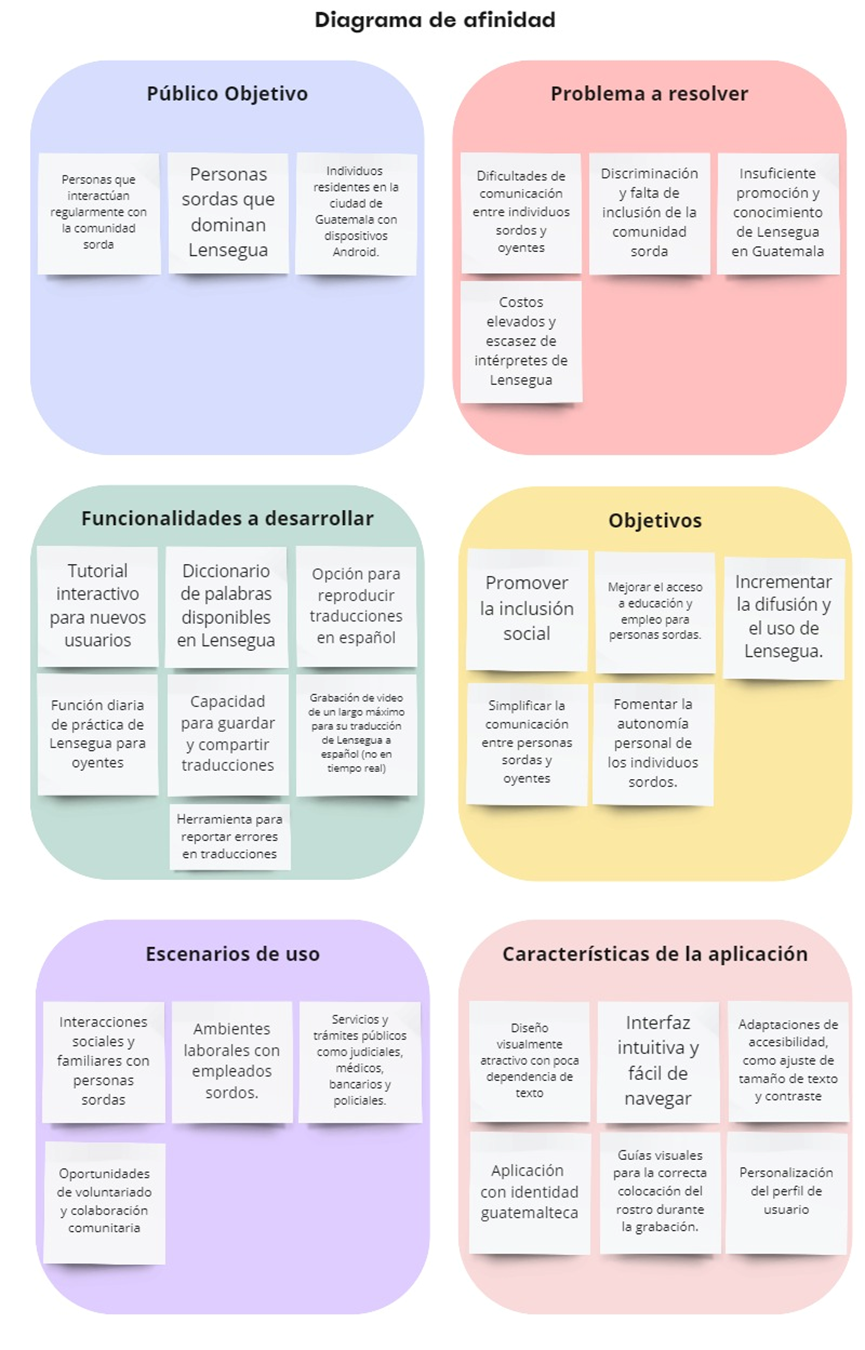
\includegraphics[width=1\linewidth]{figuras/diagrama_afinidad.png}
    \caption{Diagrama de Afinidad}
    \label{fig:enter-label}
\end{figure}

\begin{enumerate}

    \item \textbf{Público Objetivo} 
    Define a las personas que se beneficiarán directamente de la aplicación, incluyendo a aquellos que interactúan regularmente con la comunidad sorda y a las personas sordas que dominan LENSEGUA.
    \begin{itemize}
        \item Personas que interactúan regularmente con la comunidad sorda
        \item Personas sordas que dominan LENSEGUA
        \item Individuos residentes en la ciudad de Guatemala con dispositivos Android
    \end{itemize}
    
    \item \textbf{Problema a Resolver} 
    Identifica los principales desafíos que enfrenta la comunidad sorda y que la aplicación busca abordar, como las dificultades de comunicación entre sordos y oyentes, la discriminación y los altos costos de los servicios de interpretación.
    \begin{itemize}
        \item Dificultades de comunicación entre individuos sordos y oyentes
        \item Discriminación y falta de inclusión de la comunidad sorda
        \item Costos elevados y escasez de intérpretes de LENSEGUA
    \end{itemize}
    
    \item \textbf{Funcionalidades a Desarrollar} 
    Describe las características específicas que tendrá la aplicación. 
    \begin{itemize}
        \item Diccionario de palabras disponibles en LENSEGUA
        \item Función diaria de práctica de LENSEGUA para oyentes
        \item Capacidad para guardar y compartir traducciones
        \item Herramienta para reportar errores en traducciones
        \item Opción para reproducir traducciones en español
        \item Grabación de video de un largo máximo para su traducción de LENSEGUA a español (no en tiempo real)
    \end{itemize}
    
    \item \textbf{Objetivos} 
    Detalla los objetivos principales de la aplicación, como promover la inclusión social, mejorar el acceso a la educación y empleo para personas sordas, y simplificar la comunicación entre sordos y oyentes.
    \begin{itemize}
        \item Promover la inclusión social
        \item Simplificar la comunicación entre personas sordas y oyentes
        \item Mejorar el acceso a educación y empleo para personas sordas
        \item Fomentar la autonomía personal de los individuos sordos
        \item Incrementar la difusión y el uso de LENSEGUA
    \end{itemize}
    
    \item \textbf{Escenarios de Uso} 
    Enumera los diferentes contextos en los que la aplicación podría ser utilizada, incluyendo interacciones sociales, ambientes laborales, y servicios públicos como trámites médicos, bancarios y policiales.
    \begin{itemize}
        \item Interacciones sociales y familiares con personas sordas
        \item Ambientes laborales con empleados sordos
        \item Servicios y trámites públicos como judiciales, médicos, bancarios y policiales
        \item Oportunidades de voluntariado y colaboración comunitaria
    \end{itemize}
    
    \item \textbf{Características de la Aplicación} 
    Resalta aspectos del diseño y la usabilidad de la aplicación, tales como su interfaz intuitiva, el diseño visual con poca dependencia de texto y adaptaciones para accesibilidad, entre otros.
    \begin{itemize}
        \item Diseño visualmente atractivo con poca dependencia de texto
        \item Interfaz intuitiva y fácil de navegar
        \item Aplicación con identidad guatemalteca
        \item Guías visuales para la correcta colocación del rostro durante la grabación
        \item Personalización del perfil de usuario
    \end{itemize}
\end{enumerate}


\subsection{Creación de Personas}

Como parte del proceso de diseño, se han definido seis personas que representan a los usuarios finales a quienes se dirige la aplicación. 

\begin{figure} [H]
    \centering
    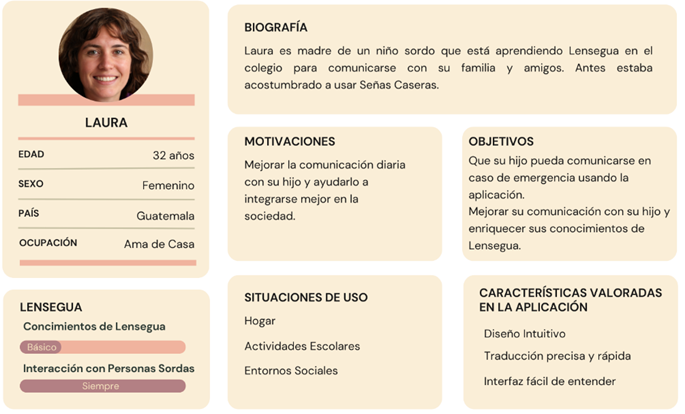
\includegraphics[width=0.8\linewidth]{figuras/persona_laura.png}
    \caption{Persona 1 - Laura}
    \label{fig:enter-label}
\end{figure}

\begin{figure} [H]
    \centering
    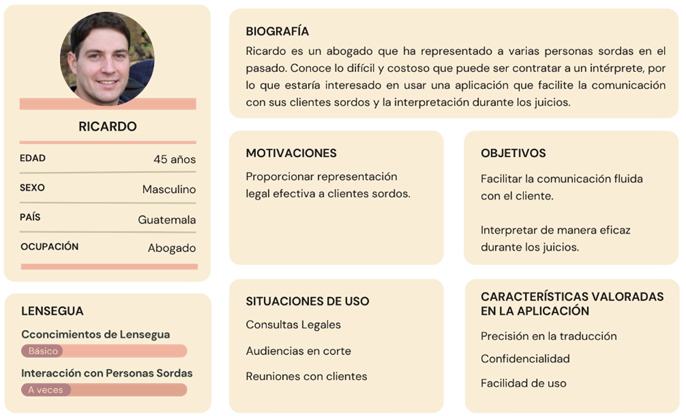
\includegraphics[width=0.8\linewidth]{figuras/ricardo_persona.png}
    \caption{Persona 2 - Ricardo}
    \label{fig:enter-label}
\end{figure}

\begin{figure} [H]
    \centering
    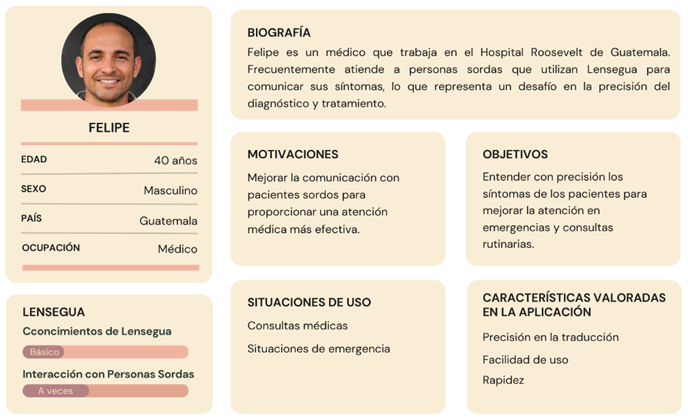
\includegraphics[width=0.8\linewidth]{figuras/felipe_persona.png}
    \caption{Persona 3 - Felipe}
    \label{fig:enter-label}
\end{figure}

\begin{figure} [H]
    \centering
    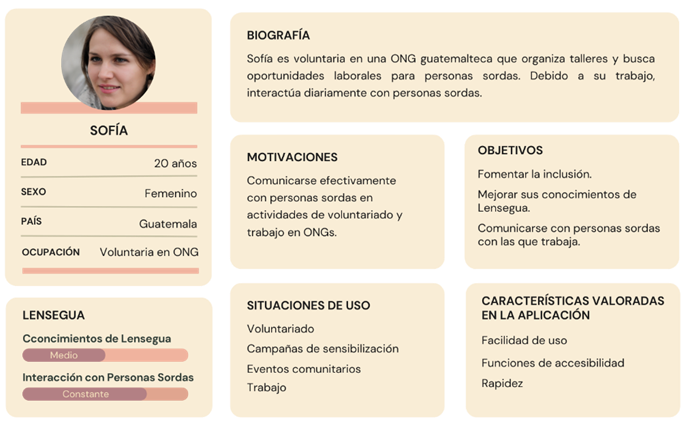
\includegraphics[width=0.8\linewidth]{figuras/sofia_persona.png}
    \caption{Persona 4 - Sofia}
    \label{fig:enter-label}
\end{figure}

\begin{figure}[H]
    \centering
    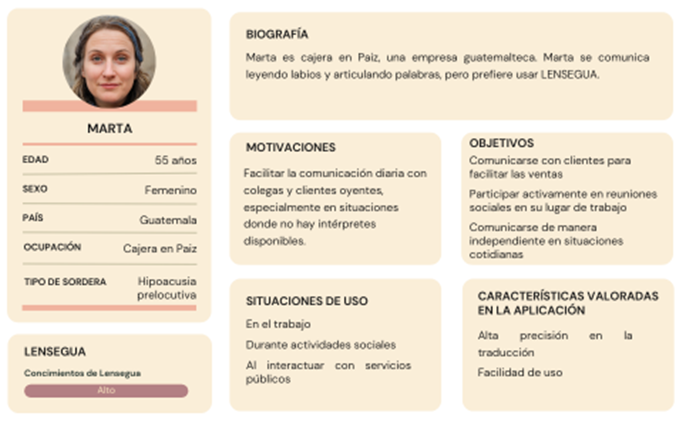
\includegraphics[width=0.8\linewidth]{figuras/marta_persona.png}
    \caption{Persona 5 - Marta}
    \label{fig:enter-label}
\end{figure}

\begin{figure} [H]
    \centering
    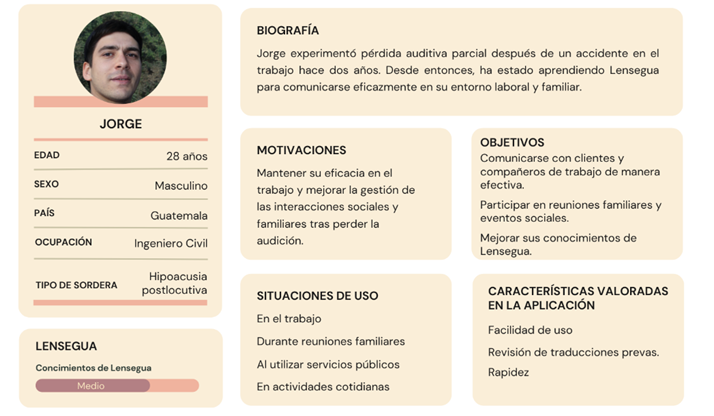
\includegraphics[width=0.8\linewidth]{figuras/jorge_persona.png}
    \caption{Persona 6 - Jorge}
    \label{fig:enter-label}
\end{figure}

% -----------------------------------------------------------------------------------------


\subsection{Creación de Mapas de Empatía}

Complementando las Personas creadas con anterioridad, se procede a crear su Mapa de Empatía respectivo para profundizar en las necesidades de los usuarios. 

\begin{figure} [H]
    \centering
    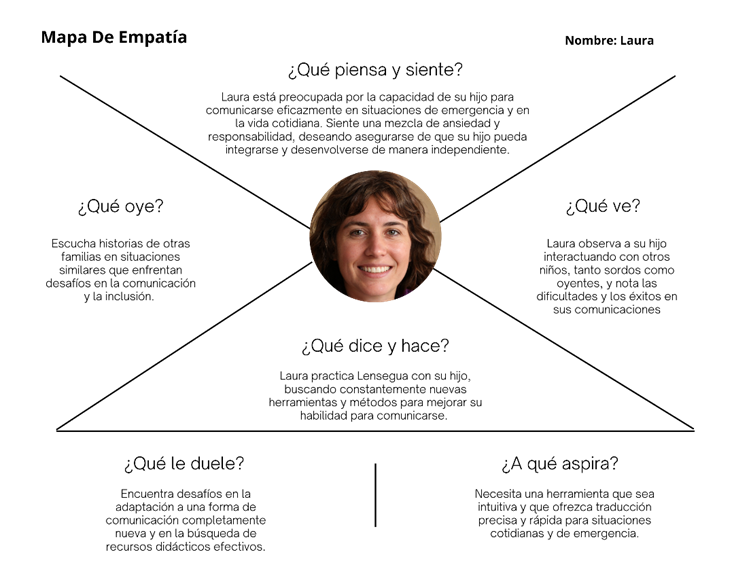
\includegraphics[width=0.9\linewidth]{figuras/mapa_empatia_laura.png}
    \caption{Mapa de Empatía - Laura}
    \label{fig:enter-label}
\end{figure}

\begin{figure} [H]
    \centering
    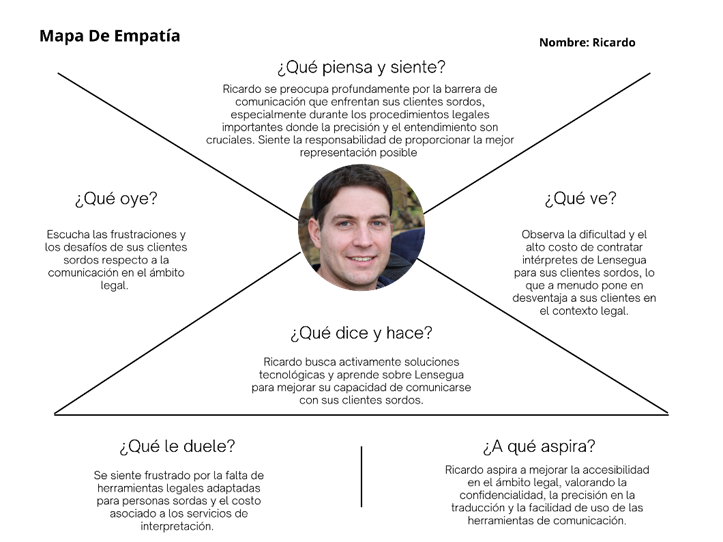
\includegraphics[width=0.9\linewidth]{figuras/mapa_empatia_ricardo.png}
    \caption{Mapa de Empatía - Ricado}
    \label{fig:enter-label}
\end{figure}

\begin{figure} [H]
    \centering
    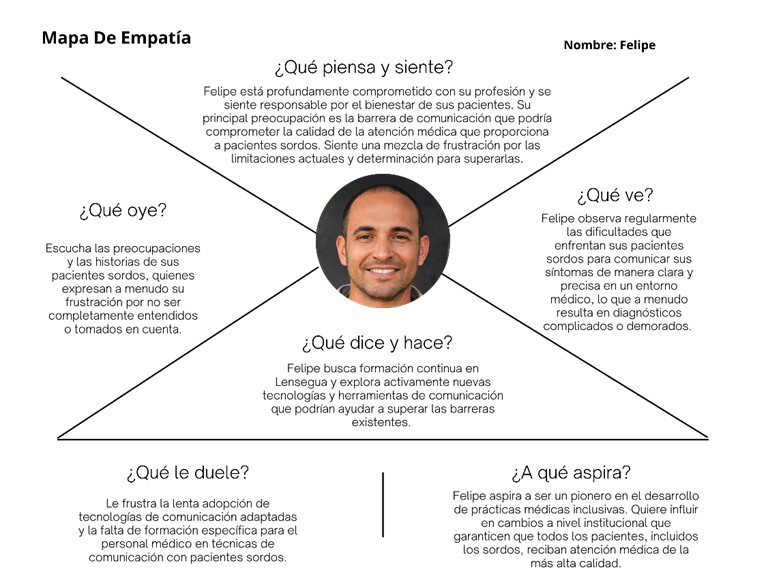
\includegraphics[width=0.9\linewidth]{figuras/mapa_empatia_felipe.png}
    \caption{Mapa de Empatía - Felipe}
    \label{fig:enter-label}
\end{figure}

\begin{figure} [H]
    \centering
    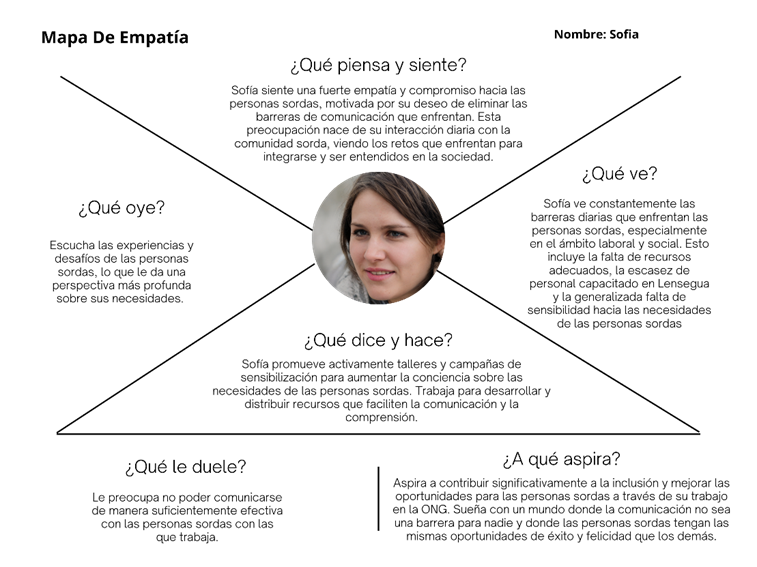
\includegraphics[width=0.9\linewidth]{figuras/mapa_empatia_sofia.png}
    \caption{Mapa de Empatía - Sofia}
    \label{fig:enter-label}
\end{figure}


\begin{figure} [H]
    \centering
    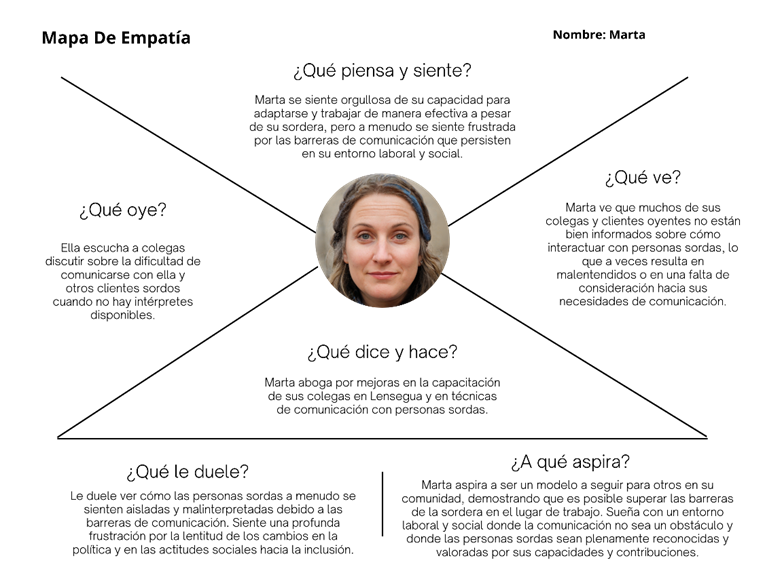
\includegraphics[width=0.9\linewidth]{figuras/mapa_empatia_marta.png}
    \caption{Mapa de Empatía - Marta}
    \label{fig:enter-label}
\end{figure}


\begin{figure} [H]
    \centering
    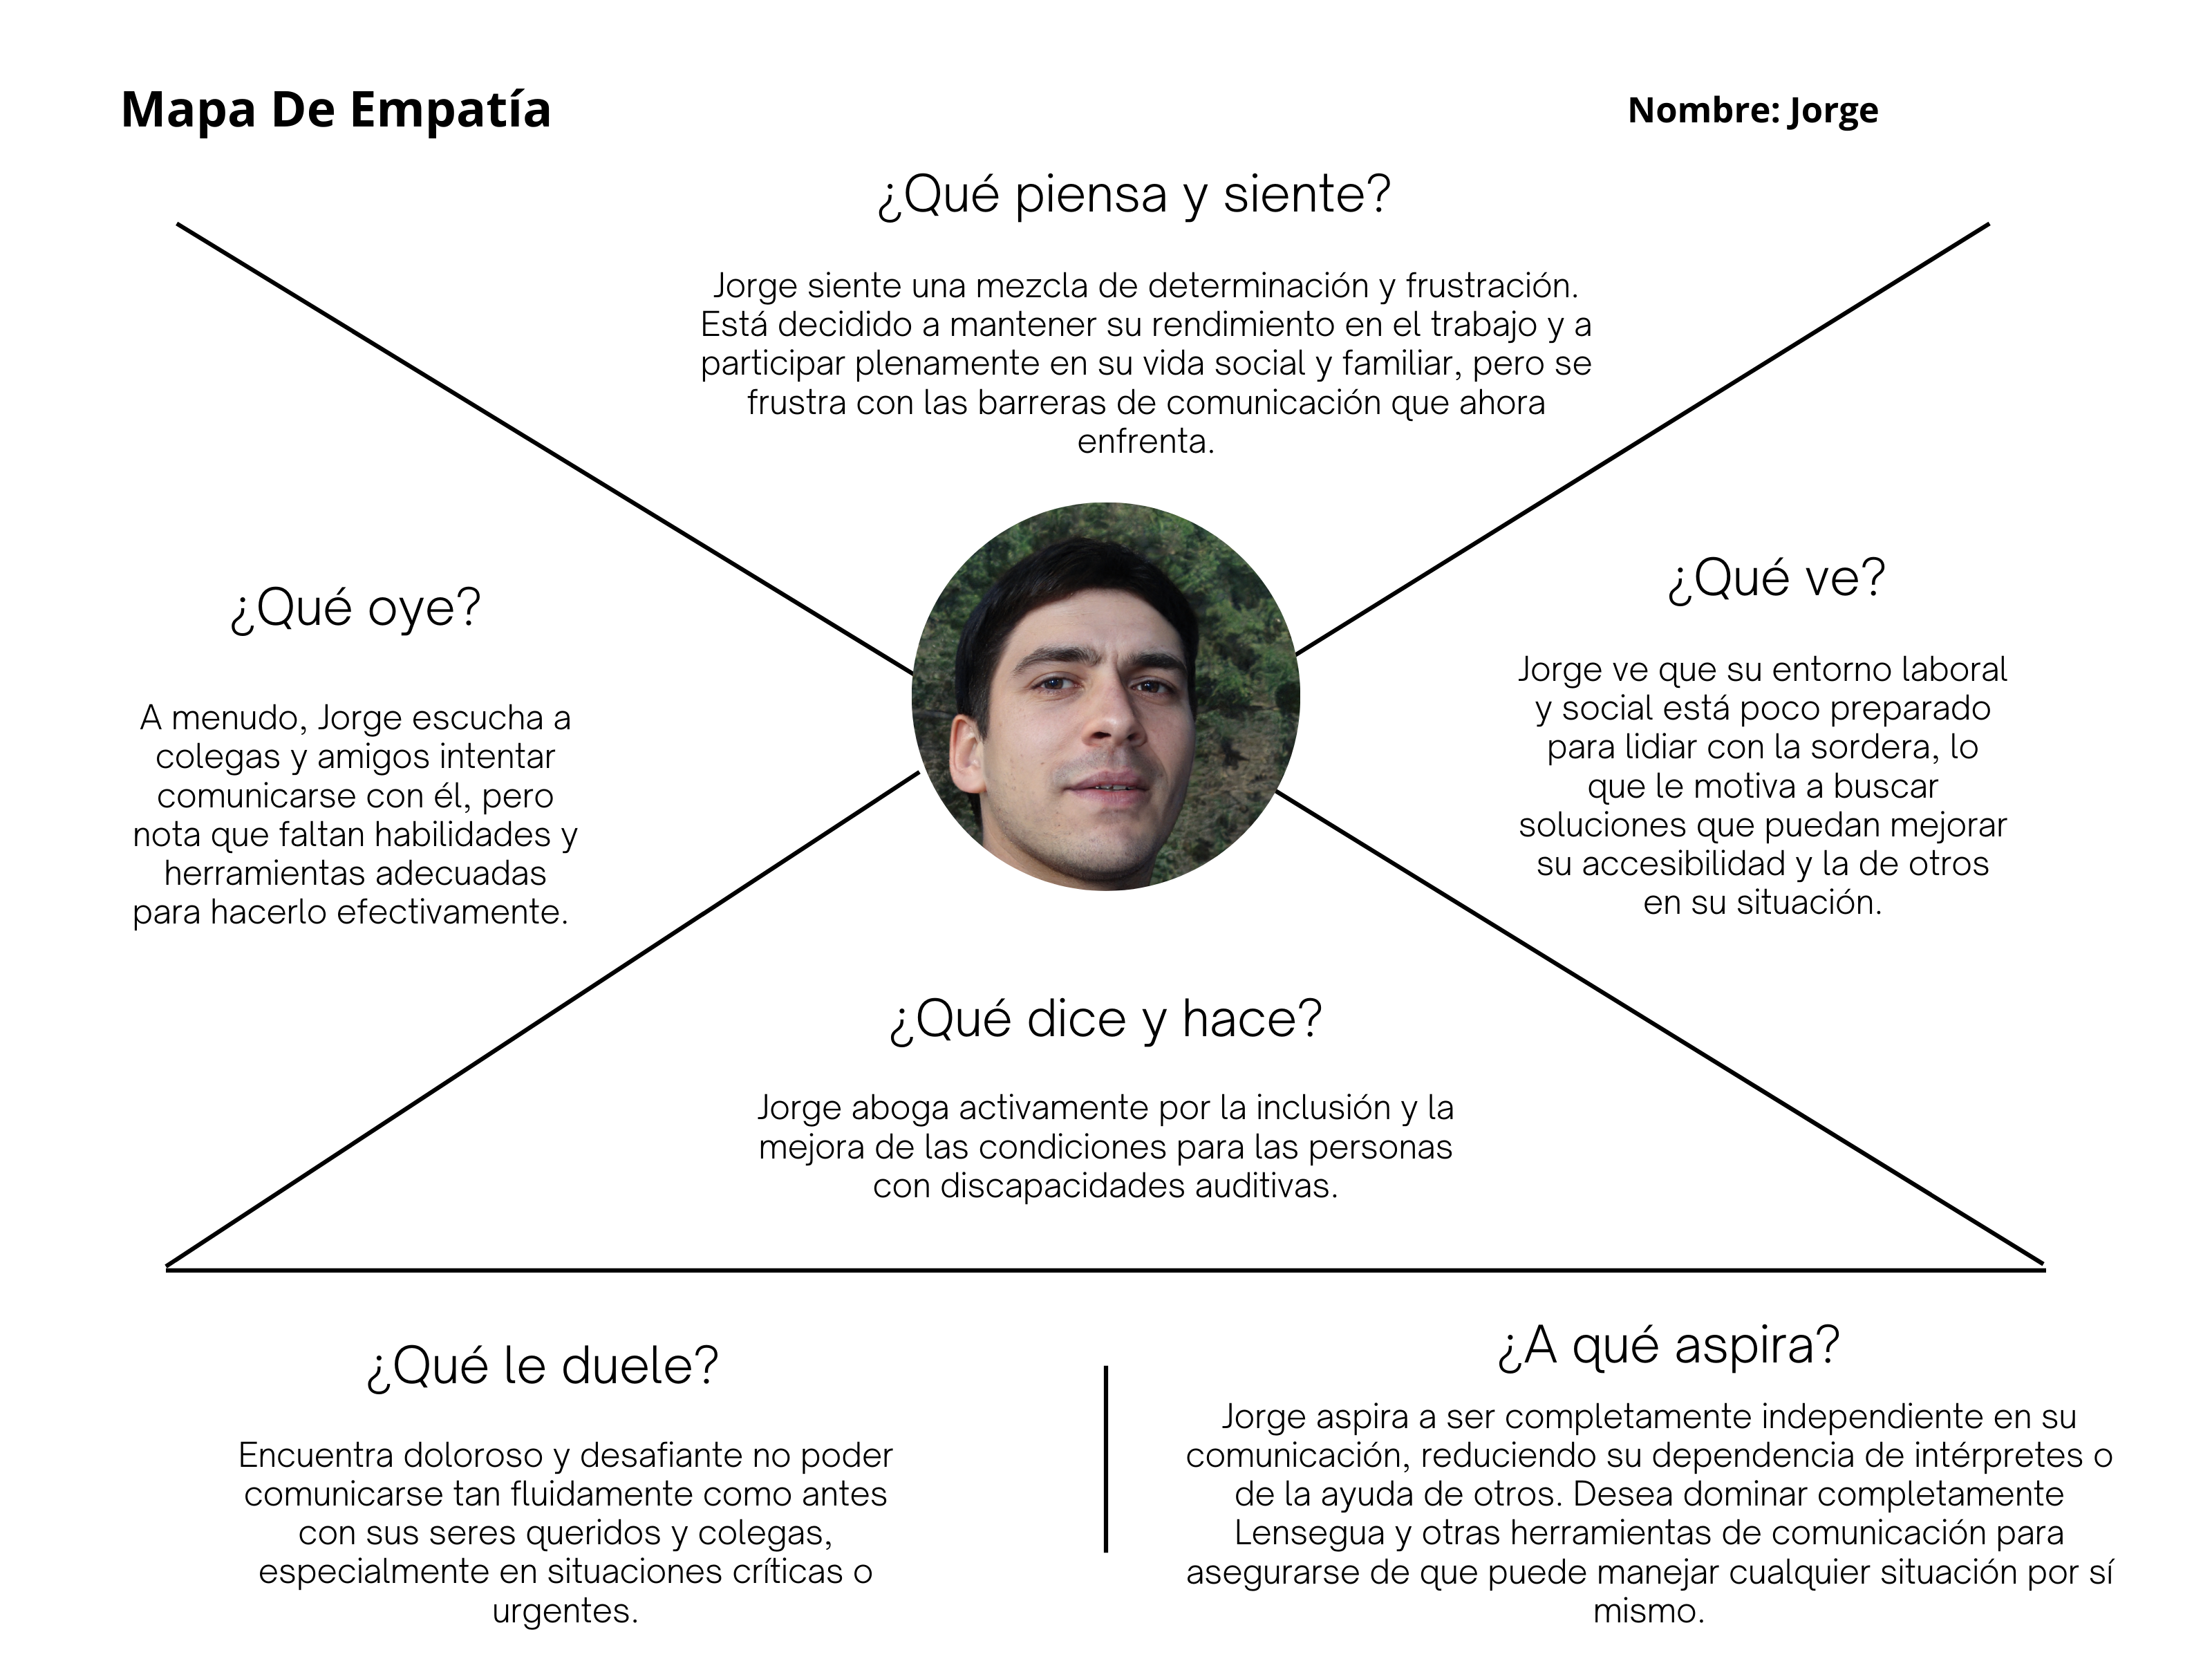
\includegraphics[width=0.9\linewidth]{figuras/mapa_empatia_jorge_correcto.png}
    \caption{Mapa de Empatía - Jorge}
    \label{fig:enter-label}
\end{figure}
% -----------------------------------------------------------------------------------------

\subsection{Planteamiento del Problema}

Inicialmente se usa Los Seis Sombreros Para Pensar, una técnica de pensamiento desarrollada por Edward de Bono en los años 80, que busca facilitar de manera creativa la resolución y el análisis de problemas desde distintos puntos de vista o perspectivas. Cada ``sombrero'' representa una dirección diferente del pensamiento y se identifica con un color específico \cite{Santos2024}.

\begin{figure} [H]
    \centering
    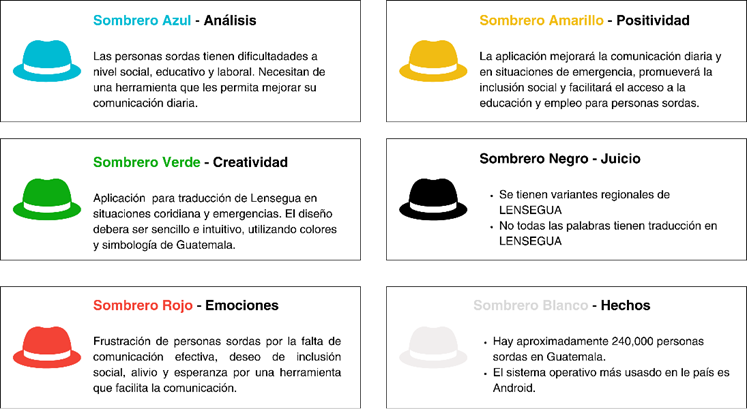
\includegraphics[width=0.8\linewidth]{figuras/sombreros.png}
    \caption{Sombreros para Pensar}
    \label{fig:enter-label}
\end{figure}


Posteriormente, se sigue el modelo W5H1 para realizar el planteamiento del problema, el cual busca ver las ideas desde varias perspectivas con el objetivo de comprender en profundidad una situación concreta \cite{Artigas2017}.

\begin{figure} [H]
    \centering
    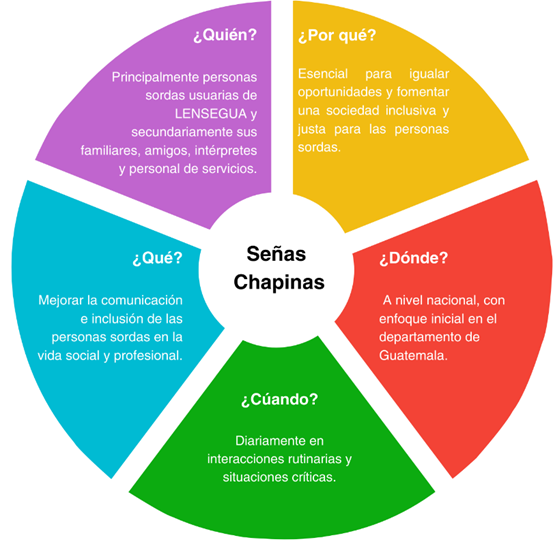
\includegraphics[width=0.6\linewidth]{figuras/w5h1.png}
    \caption{Planteamiento del Problema Señas Chapinas}
    \label{fig:enter-label}
\end{figure}

\begin{enumerate}
    \item \textbf{¿Quién?}
    \begin{enumerate}
        \item \textbf{¿A quién afecta el problema?} \\
        Afecta principalmente a personas sordas que utilizan la Lengua de Señas Guatemalteca (LENSEGUA), quienes enfrentan barreras de comunicación cotidianas.
        \item \textbf{¿Quiénes son los usuarios primarios y secundarios?}
        \begin{itemize}
            \item \textbf{Usuarios primarios:} Personas sordas, quienes dependen directamente de la comunicación efectiva para su inclusión social y profesional.
            \item \textbf{Usuarios secundarios:} Familiares, amigos, intérpretes de LENSEGUA, y personal de servicios públicos y privados que interactúan regularmente con personas sordas.
        \end{itemize}
    \end{enumerate}

    \item \textbf{¿Qué?}
    \begin{enumerate}
        \item \textbf{¿Cuáles son los límites del problema?} \\
        El problema está limitado al vocabulario esencial y de emergencia necesario para la comunicación diaria y situaciones críticas.
        \item \textbf{¿Cuál es el problema que requiere nuestra atención?} \\
        La barrera de comunicación persistente entre las personas sordas y la sociedad oyente, que limita significativamente la participación de las personas sordas en la sociedad.
        \item \textbf{¿Cuál es el objetivo final?} \\
        Facilitar la comunicación y mejorar la inclusión de la comunidad sorda en todos los aspectos de la vida social y profesional.
    \end{enumerate}

    \item \textbf{¿Cuándo?}
    \begin{enumerate}
        \item \textbf{¿Cuándo ocurre el problema?} \\
        El problema ocurre diariamente y se manifiesta en interacciones rutinarias, servicios de emergencia, entornos educativos y actividades sociales.
    \end{enumerate}

    \item \textbf{¿Dónde?}
    \begin{enumerate}
        \item \textbf{¿Dónde ocurre el problema?} \\
        El problema ocurre a lo largo de Guatemala, con un enfoque inicial en el departamento de Guatemala, debido a las variaciones dialectales de LENSEGUA en diferentes regiones.
        \item \textbf{¿Dónde se necesita enfocar más?} \\
        El enfoque inicial será en áreas urbanas donde la densidad de población y la diversidad de servicios intensifican las necesidades de comunicación efectiva.
    \end{enumerate}

    \item \textbf{¿Por qué?}
    \begin{enumerate}
        \item \textbf{¿Por qué es importante arreglar el problema?} \\
        Es importante abordar este problema para garantizar que las personas sordas en Guatemala tengan igualdad de oportunidades en su integración y participación en todos los aspectos de la vida social y profesional. Mejorar la comunicación no solo incrementa la autonomía y el bienestar de las personas sordas, sino que también contribuye a una sociedad más inclusiva y justa, donde todos los ciudadanos pueden contribuir plenamente y sin barreras.
    \end{enumerate}
\end{enumerate}

% -----------------------------------------------------------------------------------------

\subsection{Creación de Mapas de Experiencia del Cliente}

El objetivo de estos mapas es entender y abordar las necesidades y los problemas del cliente en cada etapa del proceso, identificando oportunidades para mejorar la experiencia del cliente y asegurando que cada punto de contacto con el producto sea positivo y coherente. Esto permite ver dónde se encuentran los puntos de dolor y adoptar mejoras para ofrecer una experiencia más satisfactoria y efectiva \cite{Hamond2024}.

Los mapas realizados incluyen los flujos principales a desarrollar dentro de la aplicación: 


\begin{itemize}
    \item Primera vez usando la aplicación como usuario, para identificar puntos de mejora con el primer contacto con los usuarios.

    
    \begin{figure} [H]
        \centering
        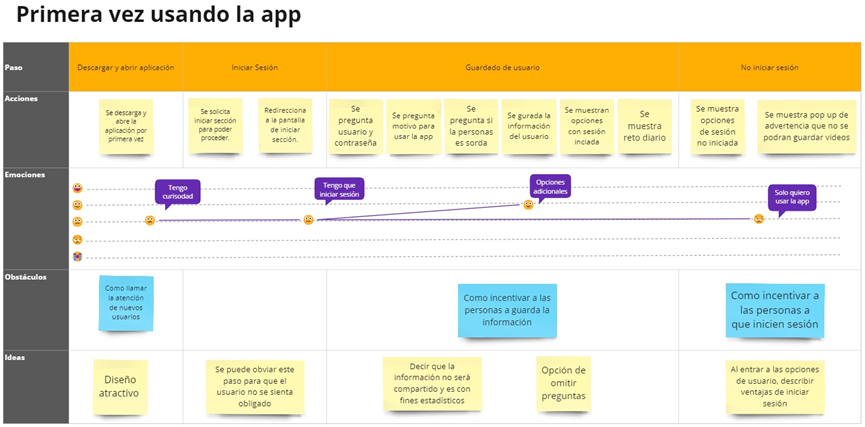
\includegraphics[width=1.1\linewidth]{figuras/mapa_exp1.png}
        \caption{Primera vez usando la aplicación}
        \label{fig:enter-label}
    \end{figure}

    
    \item Grabación de videos, para identificar cómo debe actuar la aplicación para que la funcionalidad sea sencilla.

    \begin{figure} [H]
        \centering
        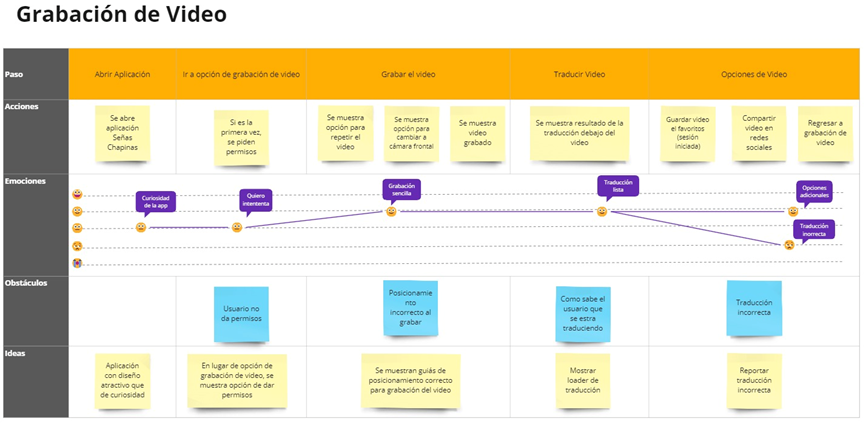
\includegraphics[width=1\linewidth]{figuras/mapa_exp2.png}
        \caption{Grabación de video}
        \label{fig:enter-label}
    \end{figure}
    
    \item Guardado de video, para analizar cómo debe realizarse el proceso.

    \begin{figure} [H]
        \centering
        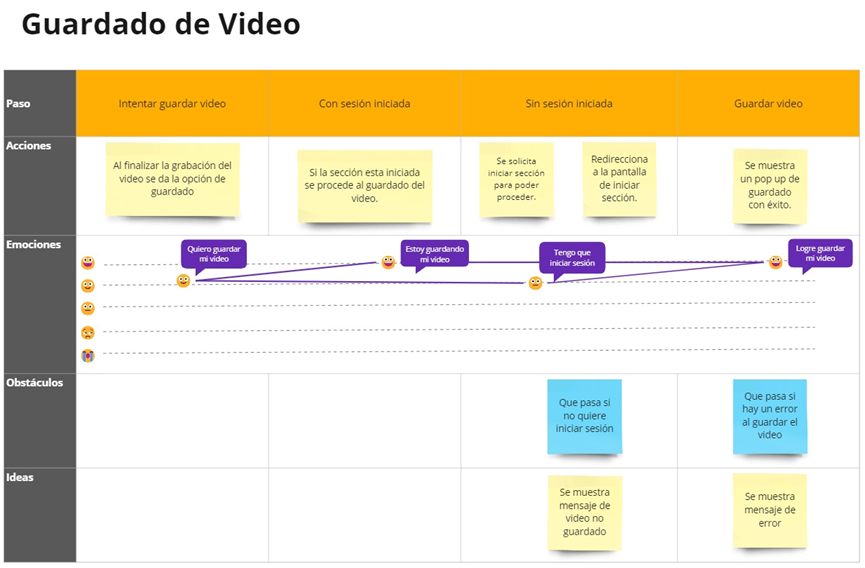
\includegraphics[width=0.9\linewidth]{figuras/mapa_exp3.png}
        \caption{Guardando Video}
        \label{fig:enter-label}
    \end{figure}
        
    \item Reporte de traducción errónea, para facilitar una manera en que los usuarios puedan ayudar a mejorar la aplicación.

    \begin{figure} [H]
        \centering
        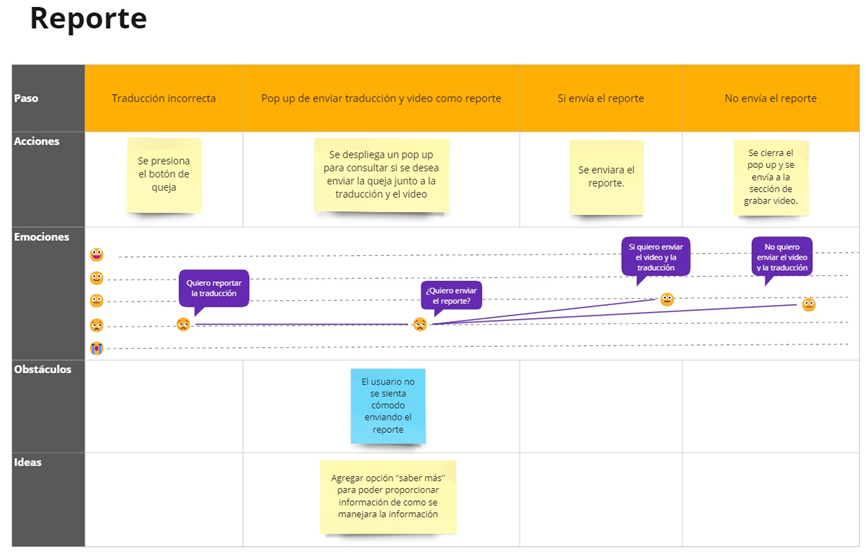
\includegraphics[width=0.95\linewidth]{figuras/mapa_exp4.png}
        \caption{Reporte}
        \label{fig:enter-label}
    \end{figure}
    
    
    \item Diccionario de palabras, para entender de qué manera los usuarios usarían esta herramienta.

    \begin{figure} [H]
        \centering
        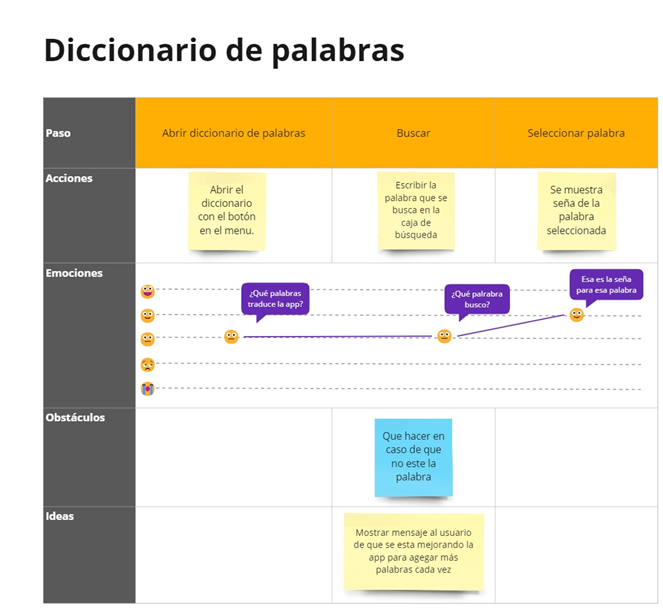
\includegraphics[width=0.7\linewidth]{figuras/mapa_exp5.png}
        \caption{Diccionario de palabras}
        \label{fig:enter-label}
    \end{figure}
    
    \item Reto diario, para identificar puntos de dolor en esta actividad.

    \begin{figure} [H]
        \centering
        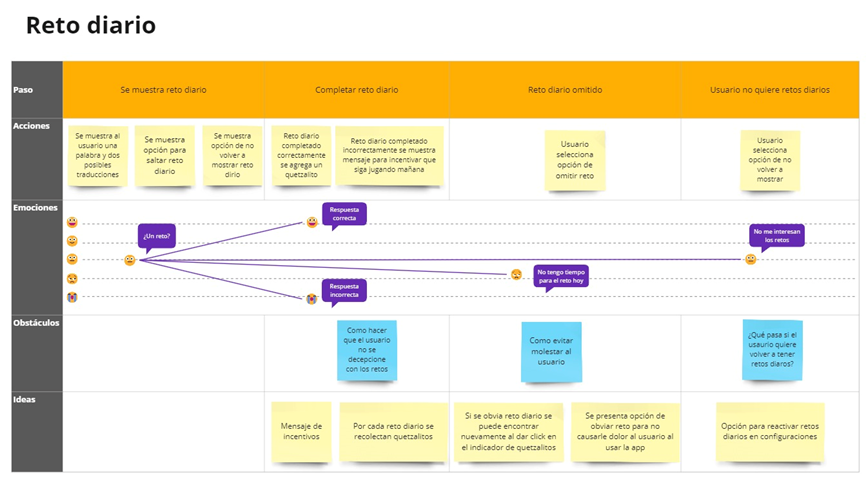
\includegraphics[width=1\linewidth]{figuras/mapa_exp6.png}
        \caption{Reto diario}
        \label{fig:enter-label}
    \end{figure}
\end{itemize}















% -----------------------------------------------------------------------------------------

\subsection{Mapa de Sitio}

Los mapas de sitio proporcionados visualizan la estructura y navegación de la aplicación ``Señas Chapinas'', facilitando un entendimiento claro de las funcionalidades disponibles para los usuarios en diferentes estados.

\begin{itemize}
    \item \textbf{Pantalla para Grabar Video}: Permite a los usuarios grabar para ser traducido a LENSEGUA. 
    \begin{itemize}
        \item \textbf{Compartir video y traducción}: Luego de traducir el video, se puede compartir el video y su traducción.
        \item \textbf{Reportar traducción incorrecta}: Si la traducción es incorrecta, los usuarios pueden reportar errores.
        \item \textbf{Guardar video}: Guardar traducciones realizadas para consultarlas nuevamente.
    \end{itemize}
    \item \textbf{Diccionario de palabras}: Pemite a los usuarios buscar vocabulario disponible para traducción. 
    
    \item \textbf{Perfil}: Acceso a configuraciones de la cuenta.
    \begin{itemize}
        \item \textbf{Información del usuario}: Muestra los detalles del usuario registrado.
        \item \textbf{Racha de retos diarios}: Muestra el progreso del usuario en retos diarios de aprendizaje.
        \item \textbf{Videos Guardados}: Acceso a videos que el usuario ha decidido guardar.
        \begin{itemize}
            \item Al seleccionar un video guardado se acceden a las mismas opciones de video traducido (compartir, reportar o grabar video).
        \end{itemize}
        \item \textbf{Configuración / Sobre la app / Ayuda}: Opciones para mejorar la experiencia del usuario en la aplicación.
        \item \textbf{Cerrar Sesión}: Permite al usuario salir de su cuenta.
    \end{itemize}
\end{itemize}

\begin{figure} [H]
    \centering
    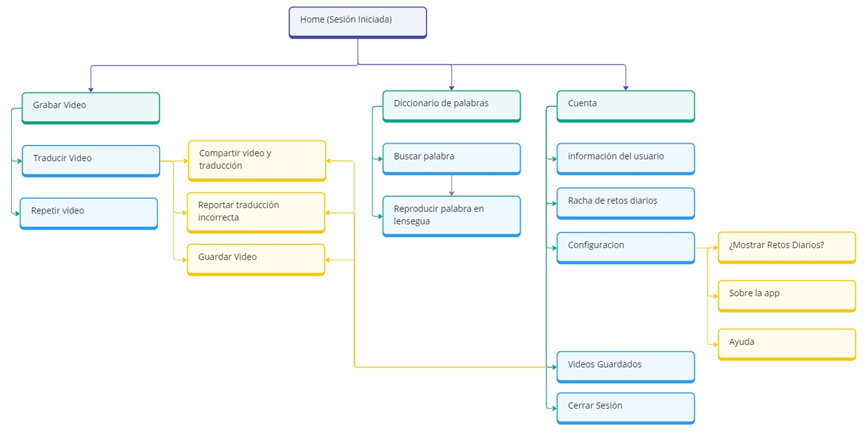
\includegraphics[width=1\linewidth]{figuras/mapa_sitio.png}
    \caption{Mapa de Sitio}
    \label{fig:enter-label}
\end{figure}

% -----------------------------------------------------------------------------------------

\subsection{Flujo de Usuarios}

En el diseño de UX, un flujo de usuarios es una representación visual de los pasos que un usuario sigue dentro de una aplicación para alcanzar un objetivo específico. Esto incluye todas las acciones, decisiones y procesos desde el punto de entrada hasta la salida \cite{Adobe2022}.

Para crear un flujo de usuarios efectivo, es crucial seguir algunos pasos detallados:

\begin{enumerate}
    \item \textbf{Comprender el viaje del cliente}: Con la información recopilada en las Personas, los Mapas de empatía y los Mapas de la experiencia del cliente, se identificaron las necesidades, motivaciones y comportamientos de los usuarios \cite{Adobe2022}.
    
    \item \textbf{Identificar y alinear los objetivos}: Cada sección de la aplicación debe tener un objetivo claro que puede diferir de los objetivos del usuario. Por lo tanto, es esencial identificar lo que los usuarios buscan lograr y alinear los objetivos de la aplicación con los de ellos para asegurar que el flujo de usuario los guíe efectivamente hacia acciones deseadas \cite{Adobe2022}.
    
    \item \textbf{Decidir la información que necesitan los usuarios}: Basado en las Personas y los Mapas del viaje del cliente, se definen los pasos necesarios que los usuarios deben seguir dentro del flujo, abordando sus puntos de dolor y proporcionando la información que buscan en cada etapa \cite{Adobe2022}.
    
    \item \textbf{Visualizar el flujo}: Finalmente, se visualiza y mapea el esquema utilizando formas para comunicar los diferentes caminos y decisiones en un flujo de usuarios \cite{Adobe2022}.
    \begin{itemize}
        \item Los óvalos representan el inicio y el final de un flujo de usuarios.
        \item Los rectángulos simbolizan un paso del proceso, una página de la aplicación.
        \item Las flechas conectan las formas y muestran la dirección del camino del usuario.
        \item Los diamantes representan decisiones que los usuarios toman en cada paso.
        \item Los paralelogramos indican dónde el usuario debe ingresar algo.
        \item El rectángulo redondeado simboliza mensajes al usuario o notificaciones dentro de la aplicación.
    \end{itemize}
    
    \item \textbf{Obtener retroalimentación}: Para mejorar la experiencia en la aplicación, se comparte con usuarios finales para identificar posibles fricciones en el flujo y encontrar formas de agilizar y mejorar las funcionalidades \cite{Adobe2022}.
\end{enumerate}

El primer Flujo de Usuario realizado es para Marta. Marta es sorda profunda y trabaja como cajera por lo que desea ofrecer sus productos de caja para obtener comisiones. Para ello graba un video y reproduce el audio de la traducción. 

\begin{figure} [H]
    \centering
    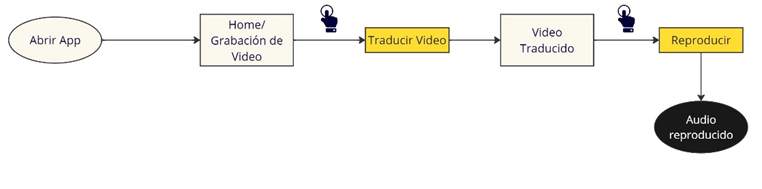
\includegraphics[width=1\linewidth]{figuras/flujo_usuario1.png}
    \caption{Grabar video}
    \label{fig:enter-label}
\end{figure}

Posteriormente se da cuenta que puede guardar el video para usarlo múltiples veces.

\begin{figure} [H]
        \centering
        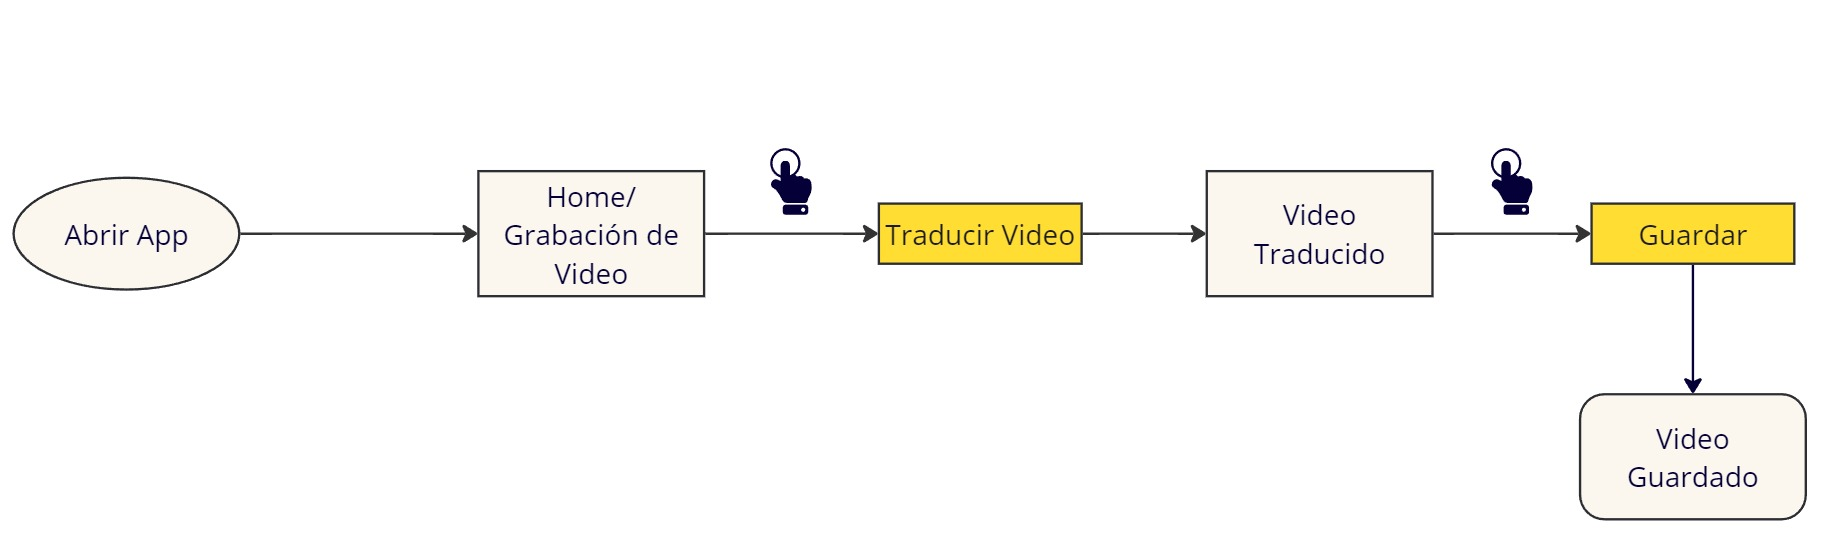
\includegraphics[width=1\linewidth]{figuras/flujo_usuario_2_correcto.jpg}
        \caption{Guardar Video}
        \label{fig:enter-label}
\end{figure}
        


\begin{figure} [H]
    \centering
    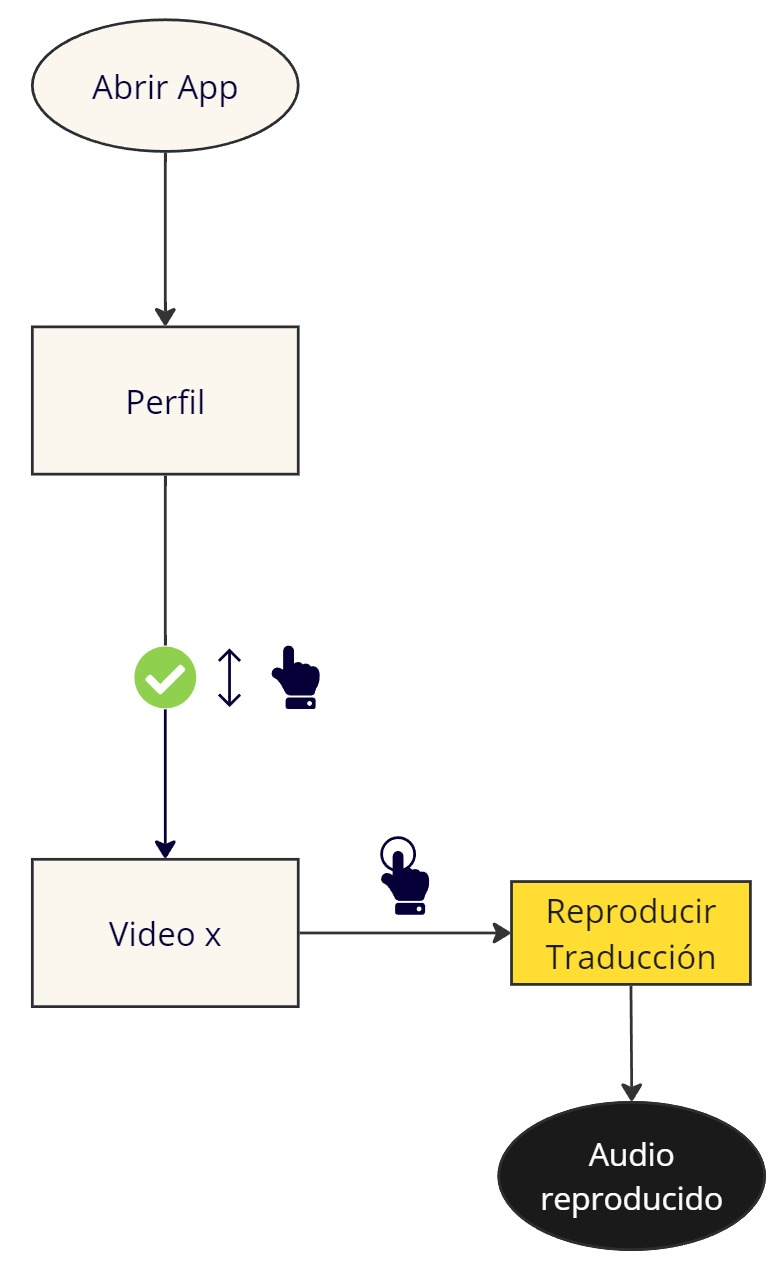
\includegraphics[width=0.4\linewidth]{figuras/flujo_usuario3.jpg}
    \caption{Abrir Video Guardado}
    \label{fig:enter-label}
\end{figure}


Por otra parte, Ricardo tiene sesiones constantemente con sus clientes, por lo que graba y guarda videos constantemente. Adicionalmente, le gusta repetir sus videos para que queden a su gusto. 

\begin{figure} [H]
    \centering
    \includegraphics[width=0.7\linewidth]{figuras/flujo_usuario4.png}
    \caption{Repertir grabación de video}
    \label{fig:enter-label}
\end{figure}


Laura a su vez, al ser madre de un hijo sordo está aprendiendo LENSEGUA. Por eso le parece importante completar los retos diarios. 


\begin{figure} [H]
    \centering
    \includegraphics[width=0.75\linewidth]{figuras/flujo_usuario6.png}
    \caption{Completar reto}
    \label{fig:enter-label}
\end{figure}


Jorge por su parte, al estar aprendiendo LENSEGUA considera muy importante tener traducciones precisas. Por ello al obtener un resultado incorrecto en su traducción, rápidamente reporta el problema.

\begin{figure} [H]
    \centering
    \includegraphics[width=1\linewidth]{figuras/flujo_usuario7.png}
    \caption{Reportar traducción}
    \label{fig:enter-label}
\end{figure}


Sofía es voluntaria por lo que al tener contacto con la comunidad sorda, despertó su interés por aprender LENSEGUA. Por eso accede al diccionario para mejorar su vocabulario. 


\begin{figure} [H]
    \centering
    \includegraphics[width=1\linewidth]{figuras/flujo_usuario8.png}
    \caption{Diccionario}
    \label{fig:enter-label}
\end{figure}


% -----------------------------------------------------------------------------------------

\subsection{Estructura Alámbrica}

Un \textit{Wireframe} o Estructura Alámbrica, es un esquema visual que representa la estructura básica de una aplicación, mostrando el diseño y la disposición de los elementos clave sin entrar en detalles sobre el estilo gráfico o contenido final. Los \textit{Wireframes} utilizan formas simples como rectángulos, líneas y texto básico para indicar elementos como encabezados, párrafos, imágenes y botones \cite{Rees2024}.

\newpage
\begin{itemize}
    \item Baja Fidelidad

        \begin{figure} [H]
            \centering
            \includegraphics[width=0.8\linewidth]{figuras/wireframe_baja.png}
            \caption{Wireframe bajo nivel}
            \label{fig:enter-label}
        \end{figure}
    
    \item Media Fidelidad

        \begin{figure} [H]
            \centering
            \includegraphics[width=0.9\linewidth]{figuras/wireframe_media.png}
            \caption{Wireframe nivel medio}
            \label{fig:enter-label}
        \end{figure}

    \newpage
    \item Alta Fidelidad

        \begin{figure}[H]
            \centering
            \includegraphics[width=1\linewidth]{figuras/fireframe_alta1.png}
            \caption{Wireframe alto nivel}
            \label{fig:enter-label}
        \end{figure}
    
\end{itemize}

Al llegar a este punto del desarrollo de la interfaz y experiencia de usuario se hace\textbf{ una primera validación con usuarios finales}. Se tuvo una reunión con varias personas de En-Señas pertenecientes tanto a la comunidad sorda como a la comunidad oyente. Tomando en cuenta los comentarios y sugerencias de esta validación, se hicieron algunas mejoras.

\begin{itemize}
    \item 
    Se ha añadido una nueva pantalla denominada ``Traducción'' cuyo propósito es permitir que las personas escriban frases en gramática LENSEGUA, que luego son traducidas a gramática española. Esta funcionalidad fue desarrollada en respuesta a los comentarios sobre cómo las personas sordas utilizan herramientas como \textit{ChatGPT} para mejorar su gramática escrita. Es importante destacar que, según los entrevistados, el nivel de comprensión lectora de una persona sorda promedio equivale aproximadamente al de un niño en tercer grado de primaria. Por lo tanto, esta herramienta no solo busca mejorar las habilidades de escritura de las personas sordas. 
    
    \item
    En la pantalla del usuario, se han añadido ahora opciones para marcar como favoritos no solo vídeos sino también traducciones.
    
    \item 
    En el diccionario, se ha implementado que las tarjetas se vuelvan interactivas, funcionando como \textit{flashcards}. Cada tarjeta muestra, por un lado, la palabra acompañada de una imagen, y por el otro, la seña correspondiente. La incorporación de imágenes fue una recomendación de intérpretes, quienes destacaron que las personas sordas tienden a ser muy visuales y que estas representaciones facilitarían significativamente su comprensión de las palabras.
    
\end{itemize}

Teniendo en cuenta estos comentarios y otras sugerencias menores, se realizaron diversas mejoras que culminaron en la creación de un nuevo \textit{Wireframe} de alto nivel.

\begin{figure} [H]
    \centering
    \includegraphics[width=1\linewidth]{figuras/wireframe_alto2.png}
    \caption{Wireframe alto nivel luego de retroalimentación}
    \label{fig:enter-label}
\end{figure}

Se consolida entonces la siguiente estructura para la aplicación:

\begin{enumerate}
    \item \textbf{Pantalla 1: Home}
    \begin{itemize}
        \item \textbf{Función Principal:} Pantalla de inicio.
        \item \textbf{Elementos:}
        \begin{itemize}
            \item Botón principal para grabar video.
            \item Botones adicionales para funcionalidades como cambiar cámara.
            \item Barra de navegación en la parte inferior con cuatro íconos para acceder a las cuatro secciones de la aplicación.
        \end{itemize}
    \end{itemize}

    \item \textbf{Pantalla 2: Traducción de video}
    \begin{itemize}
        \item \textbf{Función Principal:} Mostrar el video grabado junto con su traducción.
        \item \textbf{Elementos:}
        \begin{itemize}
            \item Área de reproducción del video.
            \item Traducción del video en la parte inferior.
            \item Botones para agregar a favoritos, compartir, repetir el video, reportar errores en la traducción y cerrar traducción.
        \end{itemize}
    \end{itemize}

    \item \textbf{Pantalla 3: Traducción de LENSEGUA a español}
    \begin{itemize}
        \item \textbf{Función Principal:} Traducir de gramática de LENSEGUA a gramática española.
        \item \textbf{Elementos:}
        \begin{itemize}
            \item Sección de LENSEGUA para escribir o pegar texto.
            \item Sección de traducción al español para copiar, reproducir o guardar la traducción.
            \item Botón para traducir/nueva traducción.
        \end{itemize}
    \end{itemize}

    \item \textbf{Pantalla 4: Perfil de usuario}
    \begin{itemize}
        \item \textbf{Función Principal:} Mostrar la información del perfil del usuario.
        \item \textbf{Elementos:}
        \begin{itemize}
            \item Ícono de perfil y nombre del usuario.
            \item Contador de días de racha de desafíos completados.
            \item Lista de videos favoritos con sus respectivas traducciones.
            \item Lista de traducciones de LENSEGUA a Español favoritas. 
        \end{itemize}
    \end{itemize}

    \item \textbf{Pantalla 5: Configuración}
    \begin{itemize}
        \item \textbf{Función Principal:} Acceder a las configuraciones de la cuenta.
        \item \textbf{Elementos:}
        \begin{itemize}
            \item Opción par obtener información sobre la aplicación. 
            \item Opción para cerrar sesión y eliminar la cuenta.
            \item Opción para desactivar los retos diarios.
        \end{itemize}
    \end{itemize}

    \item \textbf{Pantalla 6: Diccionario de palabras}
    \begin{itemize}
        \item \textbf{Función Principal:} Mostrar palabras disponibles para traducción.
        \item \textbf{Elementos:}
        \begin{itemize}
            \item Lista de palabras con sus traducciones en LENSEGUA.
            \begin{itemize}
                \item Ordenadas alfabéticamente.
                \item Botón de agregar a favoritos.
            \end{itemize}
            \item Sistema de búsqueda por palabra.
            \item Búsqueda por categorías.
        \end{itemize}
    \end{itemize}

    \item \textbf{Pantalla 7: Desafíos diarios}
    \begin{itemize}
        \item \textbf{Función Principal:} Presentar desafíos diarios de traducción.
        \item \textbf{Elementos:}
        \begin{itemize}
            \item Palabra en español
            \item 4 imágenes de posibles traducciones en LENSEGUA
            \item Opciones para omitir y cerrar el desafío.
        \end{itemize}
    \end{itemize}
\end{enumerate}


% -----------------------------------------------------------------------------------------

\subsection{Logo}

El logo de la aplicación ``Señas Chapinas'' busca simbolizar la comunidad sorda y la cultura guatemalteca. Se escogió un quetzal, el ave nacional de Guatemala, para representar el país, y manos para representar a la comunidad sorda. La evolución del logo refleja una serie de mejoras y refinamientos para lograr un diseño que comunique efectivamente estos valores.

El primer logo integraba ambos componentes: el quetzal y las manos. Las alas y la cola del quetzal se diseñaron para parecerse a manos en señas, representando así tanto la identidad cultural guatemalteca como la lengua de señas. Este diseño inicial se envió a un diseñador gráfico para recibir orientación de como mejorar su forma y funcionalidad.

\begin{figure} [H]
    \centering
    \includegraphics[width=0.75\linewidth]{figuras/primerLogo.png}
    \caption{Primer Logo}
    \label{fig:enter-label}
\end{figure}

El segundo diseño mantuvo la misma idea pero fue vectorizado, simplificado y mejorado en términos de legibilidad y estilo. La vectorización permitió un diseño más limpio y adaptable a diferentes tamaños y medios.

\begin{figure} [H]
    \centering
    \includegraphics[width=0.4\linewidth]{figuras/logo2.png}
    \caption{Logo vectorizado}
    \label{fig:enter-label}
\end{figure}


Para el tercer diseño, se solicitó la colaboración de una diseñadora gráfica con el fin de modernizar el logo. Como resultado, se decidió utilizar solo una mano en lugar de dos, simplificando y actualizando el concepto visual.

\begin{figure} [H]
    \centering
    \includegraphics[width=0.4\linewidth]{figuras/logo3.png}
    \caption{Logo modernizado}
    \label{fig:enter-label}
\end{figure}

En colaboración con la diseñadora gráfica se seleccionaron los colores del logo, incorporando tonos verde, rojo y amarillo que evocan las características distintivas del quetzal y reflejan la identidad cultural guatemalteca. Estos colores no solo realzan visualmente el logo, sino que también fortalecen su vínculo con el patrimonio nacional.

\begin{figure} [H]
    \centering
    \includegraphics[width=0.4\linewidth]{figuras/logo4.png}
    \caption{Logo con colores}
    \label{fig:enter-label}
\end{figure}

Finalmente, se logró el diseño definitivo: un logo colorido y moderno que refleja la cultura de Guatemala a través del símbolo del quetzal y representa a la comunidad sorda con la imagen de una mano utilizando LENSEGUA. Este logo combina simplicidad, modernidad y simbolismo cultural, proporcionando una representación atractiva y efectiva para la aplicación. 


\begin{figure} [H]
    \centering
    \includegraphics[width=0.4\linewidth]{figuras/logo_final.png}
    \caption{Logo Señas Chapinas}
    \label{fig:enter-label}
\end{figure}



% -----------------------------------------------------------------------------------------

\subsection{Paleta de Colores}


Los colores seleccionados para el logo son los siguientes:


\begin{itemize}
    
    \item \textbf{Verde Quetzal (\#00973A):} Este color representa al quetzal y simboliza vida y esperanza. 
       
    \item \textbf{Rojo (\#E20613):}  Su uso en la aplicación es para indicar errores o acciones importantes, facilitando al usuario identificar problemas o acciones críticas dentro de la aplicación.

    \item \textbf{Verde Lima (\#93C01F):} Se utiliza para dar mas detalle al quetzal y para el título de la aplicación porque tiene mayor contraste con el azul del fondo. 
    
    \item \textbf{Amarillo (\#FFDD00):}) Usado para destacar el pico del quetzal en el logo, este amarillo no solo contrasta eficazmente con los verdes, sino que también simboliza felicidad y acción. 

    \item \textbf{Azul (\#29235C):}) Aunque el azul tradicional de la bandera de Guatemala es más claro, se ha seleccionado un tono azul oscuro para conferir profundidad y seriedad al logo
    
\end{itemize}

\begin{figure} [H]
    \centering
    \includegraphics[width=0.25\linewidth]{figuras/paleta_colores_logo.png}
    \caption{Paleta de colores logo}
    \label{fig:enter-label}
\end{figure}


Con base a estos colores, también se seleccionaron los colores para la aplicación, buscando no solo impacto visual, sino también  fortalecer la conexión con la identidad cultural guatemalteca.

\begin{itemize}
    \item \textbf{Azul (\#29235C):} Se utiliza principalmente como color para texto de la aplicación. Ofrece legibilidad y una sensación de seguridad y confianza.  
    
    \item \textbf{Verde Quetzal (\#00973A):} Se usa para botones y títulos, aportando vitalidad y energía a la interfaz. 
       
    \item \textbf{Rojo (\#E20613):} Se utuliza para indicar errores o acciones importantes, facilitando al usuario identificar problemas o acciones críticas dentro de la aplicación.

    \item \textbf{Blanco Crema (\#F5F5F5):} Se utiliza como fondo para la aplicación. En lugar del blanco puro, este tono crema proporciona una suavidad que puede ser menos agresiva a la vista. 
    
    \item \textbf{Gris Carbón (\#323232):} Se utiliza principalmente como fondo de pantallas de temporales. Es un color neutro elegido específicamente para minimizar las distracciones y evitar que los usuarios permanezcan en estas pantallas transitorias por más tiempo del necesario, a diferencia del uso de los colores azul y blanco en otras secciones de la aplicación, que buscan captar y mantener la atención del usuario.

\begin{figure} [H]
    \centering
    \includegraphics[width=0.6\linewidth]{figuras/paleta_colores.png}
    \caption{Paleta de colores aplicación}
    \label{fig:enter-label}
\end{figure}

    
    
\end{itemize}

Con base a la paleta de colores del logo, se obtienen colores pastel utilizados para el quetzal de perfil del usuario y las opciones del reto diario:

\begin{itemize}

    \item Aqua Pastel (\#37B7C3)
    \item Azul Pastel (\#83B4FF)
    \item Verde Pastel (\#8DC249)
    \item Amarillo Pastel (\#FCB424)

\end{itemize}

\begin{figure} [H]
    \centering
    \includegraphics[width=0.5\linewidth]{figuras/paleta_colores_quetzal.png}
    \caption{Paleta Colores Perfil}
    \label{fig:enter-label}
\end{figure}

Asimismo también se comprueban contrastes de los colores seleccionados:

\begin{itemize}

    \item \textbf{Azul y Blanco:} Los colores azul y blanco seleccionados presentan un contraste óptimo, lo cual justifica su uso como fondo y texto principales en la aplicación. 

    \begin{figure} [H]
        \centering
        \includegraphics[width=0.6\linewidth]{figuras/contraste_azul_blanco.png}
        \caption{Contraste blanco y azul}
        \label{fig:enter-label}
    \end{figure}


    \begin{figure} [H]
        \centering
        \includegraphics[width=0.6\linewidth]{figuras/contraste_blanco_azul.png}
        \caption{Contraste azul y blanco}
        \label{fig:enter-label}
    \end{figure}

  
    \item \textbf{Contraste gris y blanco:} Los colores gris y blanco seleccionados ofrecen un contraste adecuado, lo cual los hace idóneos para su uso en las pantallas temporales. 

    \begin{figure} [H]
        \centering
        \includegraphics[width=0.6\linewidth]{figuras/contraste_gris_blanco.png}
        \caption{Contraste gris y blanco}
        \label{fig:enter-label}
    \end{figure}
    
    
    \item \textbf{Constraste blanco y rojo:}  Aunque el contraste entre blanco y rojo no es tan alto como en otros casos, aún cumple con los requisitos mínimos recomendados. Este se utiliza exclusivamente en situaciones necesarias para alertar al usuario sobre una acción crítica.

    \begin{figure} [H]
        \centering
        \includegraphics[width=0.6\linewidth]{figuras/contraste_blanco_rojo.png}
        \caption{Contraste blanco y rojo}
        \label{fig:enter-label}
    \end{figure}
    
    \item \textbf{Contraste verde quetzal y azul:} El contraste entre el verde quetzal es ligeramente inferior al nivel recomendado. Por esta razón, se empleará únicamente para elementos destacados como títulos grandes, botones y el logo, donde la legibilidad sigue siendo efectiva a pesar del menor contraste. 
   
    \begin{figure} [H]
        \centering
        \includegraphics[width=0.6\linewidth]{figuras/contraste_azul_verde.png}
        \caption{Constraste verde quetzal y azul}
        \label{fig:enter-label}
    \end{figure}

    \item \textbf{Contraste verde claro y azul:} El contraste entre el verde claro y el azul cumple con las normas recomendadas, razón por la cual se ha seleccionado para el título de la aplicación
    
    \begin{figure} [H]
        \centering
        \includegraphics[width=0.6\linewidth]{figuras/contraste_verde_claro_azul.png}
        \caption{Constraste verde claro y azul}
        \label{fig:enter-label}
    \end{figure}
        

\end{itemize}


% -----------------------------------------------------------------------------------------

\subsection{Tipografía}

La tipografía recomendada por la diseñadora gráfica para el logo de ``Señas Chapinas'' fue Adonide Bold. Esta elección se justifica por su claridad y modernidad, cualidades que reflejan la simplicidad y accesibilidad que la aplicación busca transmitir. Adonide Bold es una fuente sans-serif que ofrece un aspecto limpio y profesional, ideal para destacar en logotipos y cabeceras por su legibilidad y presencia  \cite{AdonideFont}.

Con base a esa tipografía y al contexto de la aplicación, se decide utilizar Nunito para el contenido de la misma. Nunito, también una sans-serif disponible gratuitamente en \textit{Google Fonts}, es conocida por sus curvas suaves y su legibilidad en interfaces digitales, lo que la hace ideal para textos largos y elementos de interfaz de usuario en aplicaciones móviles. Su diseño amigable y accesible complementa perfectamente la estética introducida por Adonide Bold en el logo, asegurando coherencia visual y facilitando la experiencia del usuario al navegar por la aplicación. Esta elección refuerza el objetivo de la aplicación de ser accesible y fácil de usar, elementos cruciales para una herramienta destinada a mejorar la comunicación en la comunidad sorda \cite{Design2024}.

\begin{figure} [H]
    \centering
    \includegraphics[width=0.75\linewidth]{figuras/tipografia.png}
    \caption{Tipografía Nunito}
    \label{fig:enter-label}
\end{figure}

% -----------------------------------------------------------------------------------------

\subsection{Prototipos}

Al concluir la fase de diseño UX/UI, se han definido claramente las necesidades de los usuarios, así como los flujos principales de la aplicación. Durante este proceso, también se seleccionaron cuidadosamente los colores y la tipografía que mejor se adaptan a la experiencia del usuario, garantizando así coherencia visual y funcionalidad. Con estos elementos bien establecidos, el siguiente paso ha sido la creación de prototipos detallados en Figma. Este enfoque permite simular la interacción del usuario con la aplicación.

\subsubsection{Prototipo de Bajo Nivel}
Este primer prototipo tiene como objetivo demostrar la funcionalidad general de la aplicación sin enfocarse en el diseño de colores, presentando una estructura básica. Para ver el diseño con más detalles consultar: \href{https://www.figma.com/design/d7NOw36r1mUY7qDBIveJ2K/Se%C3%B1as-Chapinas?node-id=45-820&node-type=SECTION&t=luJsnsyUNaEJGP24-0}{Figma}.

\begin{itemize}
    \item \textbf{Barra de Navegación:} Contiene las opciones de ``Video'', ``Traductor'', ``Diccionario'' y ``Perfil''. La opción seleccionada se destaca visualmente sobre las demás.
    
    \item \textbf{Pantalla de Inicio:} Ofrece la función principal de grabar video. Al presionar el botón correspondiente, el video comienza a grabarse.
    
    \item \textbf{Pantalla de Video:} Muestra el video grabado junto con opciones para reportar errores, agregar a favoritos, compartir, repetir, utilizar el altavoz y cerrar. Las traducciones en español y LENSEGUA se muestran en la parte inferior.
    
    \item \textbf{Reporte de Traducción:} Un modal que permite al usuario reportar errores en la traducción. Antes de continuar, se solicita revisar el diccionario. Luego, el usuario puede proceder con el reporte.
    
    \item \textbf{Traductor:} Al ingresar, se presenta un área para escribir o pegar texto en LENSEGUA. El botón de traducción está deshabilitado hasta que el usuario ingrese el texto. Una vez ingresado, el botón se habilita, y al presionarlo, se muestra la traducción al español junto con las opciones de copiar, escuchar con el altavoz, agregar a favoritos o realizar una nueva traducción.
    
    \item \textbf{Diccionario:} Muestra tarjetas redondeadas que representan las palabras disponibles. Las tarjetas se pueden agregar a favoritos. En la parte superior, se incluye una barra de búsqueda y la opción de seleccionar por categorías. Además, cuenta con una barra de desplazamiento para navegar entre las tarjetas ordenadas alfabéticamente.
    
    \item \textbf{Perfil del Usuario:} Muestra una imagen de perfil, el nombre del usuario y un contador de días consecutivos de desafíos completados. También incluye un ícono de configuración en la parte superior para acceder a ajustes. La pantalla presenta una barra de pestañas que permite alternar entre los videos favoritos y las traducciones favoritas.
    
    \item \textbf{Configuraciones:} Ofrece opciones para cambiar la contraseña, cerrar sesión, eliminar la cuenta y acceder a información sobre la aplicación. También permite activar o desactivar los retos diarios y consultar la versión actual de la aplicación.
    
    \item \textbf{Retos Diarios:} Presenta cuatro imágenes como opciones de respuesta para una palabra en LENSEGUA. El usuario puede elegir una respuesta, o bien, cerrar u omitir el reto. Las opciones se presentan en un diálogo interactivo.
\end{itemize}

Cabe destacar que el diseño del primer prototipo se caracteriza por su simplicidad e intuición, con un uso mínimo de texto para facilitar la navegación. Basado en las recomendaciones de los usuarios finales, se utilizaron como referencia aplicaciones que ellos consideran fáciles de usar, adaptando y personalizando el diseño a la identidad y necesidades únicas de la aplicación 'Señas Chapinas'. Un ejemplo de ello es la disposición de las opciones en la pantalla de video, que recuerda a la aplicación \textit{TikTok}.

\begin{figure} [H]
    \centering
    \includegraphics[width=1\linewidth]{figuras/Prototipo1.png}
    \caption{Primer Prototipo}
    \label{fig:primer_prototipo}
\end{figure}

\subsubsection{Prototipo de Nivel Medio}

Tras presentar el primer prototipo a los usuarios finales, se realizaron algunos ajustes visuales menores, como la modificación del tamaño del texto y de los íconos. Después de implementar estos cambios y obtener la aprobación de los usuarios, se desarrolló el segundo prototipo. Este incluyó pantallas para el inicio de sesión y la creación de cuenta, una pantalla de inicio, una pantalla para cambio de contraseña, y una pantalla con descripción de la aplicación. Además, se empezó a integrar color y mejorar la navegación. Para analizar con más detalle revisar: \href{https://www.figma.com/design/d7NOw36r1mUY7qDBIveJ2K/Se%C3%B1as-Chapinas?node-id=275-15737&node-type=CANVAS&t=ua1wEji5yxVRI6ES-0}{Figma} 


\begin{figure} [H]
    \centering
    \includegraphics[width=1\linewidth]{figuras/segundo_prototipo.png}
    \caption{Segundo Prototipo}
    \label{fig:segundo_prototipo}
\end{figure}

\subsubsection{Prototipo de Alto Nivel}

El tercer prototipo muestra ya el diseño completo de la aplicación, para ver mas a detalle revisar \href{https://www.figma.com/design/d7NOw36r1mUY7qDBIveJ2K/Se%C3%B1as-Chapinas?node-id=322-1684&node-type=CANVAS&t=ua1wEji5yxVRI6ES-0}{Figma}:

\begin{itemize}
    \item \textbf{Pantalla de \textit{Splash}:} Fondo azul con el logo y nombre de la aplicación.
  
    \item \textbf{Pantalla de Inicio:} En la parte superior se muestra el logo y el nombre, seguido por el eslogan en español y LENSEGUA. También se incluyen los botones ``Empezar Ahora'', que lleva a la creación de cuenta, y ``Ya tengo una cuenta'', para iniciar sesión.
  
    \item \textbf{Creación de Cuenta:} El logo y el nombre se presentan en la parte superior azul, mientras que en la parte inferior blanca se muestran los campos para ingresar el correo, la contraseña y la confirmación de contraseña. Se incluyen dos botones: ``Empezar Ahora'', que continúa con el flujo, y ``Ya tengo una cuenta'', para redirigir al login.
  
    \item \textbf{Grabación de Video:} Muestra la simulación de la toma de video, con un botón de grabación al centro y una barra de navegación inferior que incluye las opciones de video, traducción, diccionario y perfil.

    \item \textbf{Video:} Presenta una simulación del video grabado con opciones en la parte superior para reportar, agregar a favoritos, compartir y repetir el video. En la parte inferior se muestra la traducción en LENSEGUA y español. Se usa iconografía estándar en lugar de texto para facilitar la navegación a las personas sordas.

    \item \textbf{Reportar:} A diferencia del primer prototipo, ya no se utiliza un modal, sino un \textit{bottom sheet}, de acuerdo con las recomendaciones de un experto en diseño, ya que es más dinámico, moderno y menos intrusivo. El título se presenta en rojo para resaltar que es una acción crítica. Se le pide al usuario que revise si la palabra existe en el diccionario antes de reportarla, y se muestran botones con el ícono del diccionario utilizado en la barra de navegación, cumpliendo con la solicitud de las personas sordas de utilizar iconografía y no solo texto. El botón de reportar también es rojo, ya que se trata de una acción crítica. Al finalizar el flujo de reporte, se muestra un mensaje confirmando que el reporte ha sido generado.

    \item \textbf{Traductor:} A diferencia del primer prototipo, se introduce un fondo azul en el área de ingreso de texto en LENSEGUA y un fondo blanco para el texto traducido en español. Se ha añadido un límite máximo de palabras para ingresar, a solicitud del equipo de inteligencia artificial. Al igual que en el primer prototipo, el botón de traducir es verde, para resaltar la acción. Este permanece deshabilitado hasta que el usuario ingrese texto en LENSEGUA. Al hacer clic en el botón de traducir, se bloquea la edición del texto en LENSEGUA, y el botón cambia a "Nueva Traducción". Posteriormente, se muestra la traducción en español y las opciones para copiar, usar el altavoz y agregar a favoritos, manteniendo el uso de iconografía en lugar de texto.

    \item \textbf{Diccionario:} El diseño de las tarjetas ha cambiado ligeramente en comparación con el primer prototipo. Ahora se incluye un ícono que indica que la tarjeta se puede voltear, y se ha reducido el redondeado y sombreado de las tarjetas. La barra de búsqueda se mantiene en la parte superior. En las categorías, se ha agregado la sección de favoritos con un ícono de corazón, manteniendo la coherencia de la aplicación, donde los favoritos siempre se representan con un corazón. También se ha incorporado un estado vacío \textit{(empty state)} para cuando no haya resultados en la búsqueda o no se hayan guardado favoritos.

    \item \textbf{Perfil:} A diferencia del primer prototipo, donde el usuario podía seleccionar su propia imagen de perfil, se decidió que la aplicación asignará un color al quetzal del logo, para cada usuario. Se sigue mostrando el nombre del usuario y la racha de desafíos en la parte inferior de la imagen de perfil. Además, el diseño de los favoritos, tanto de videos como de traducciones, ha sido ajustado para añadir más formalidad y dinamismo a la aplicación. También se incluyen flujos para borrar favoritos y pantallas de estado vacío cuando no haya favoritos guardados.

    \item \textbf{Configuración:} El diseño de la sección de configuración ha cambiado respecto al primer prototipo. Ahora incluye subconjuntos de opciones e iconografía para facilitar la navegación del usuario. Además, se ha añadido el flujo de eliminación de cuenta, que se muestra mediante un \textit{bottom sheet} con un título en rojo, dado que es una acción crítica. El diseño de la sección ``Acerca de la Aplicación'' también ha sido ajustado ligeramente y se han añadido los colaboradores.

    \item \textbf{Reto Diario:} El diseño de la pantalla de retos diarios fue uno de los más desafiantes, ya que no se sabía cómo proporcionar retroalimentación clara cuando el usuario seleccionaba una opción incorrecta, ni cómo manejar las rachas de forma visual. Finalmente, se decidió por una pantalla que en la parte superior muestra la racha actual, un título llamativo, y la palabra objetivo a seleccionar en las tarjetas. Las tarjetas utilizan colores pastel, y en la parte inferior se encuentra la opción de omitir. Cuando la respuesta es correcta, se añade un punto a la racha y aparece una animación de confeti. Si la respuesta es incorrecta, la racha se restablece a cero, el ícono de la racha cambia de color, y se muestra un mensaje para motivar al usuario a intentarlo de nuevo. La tarjeta correcta se muestra en un color más claro que las demás después de que el usuario haya seleccionado una opción. A diferencia del primer prototipo, esta es una pantalla completa y no un modal.

     \item \textbf{Cambio de Contraseña:} Al igual que en el primer prototipo, se muestra el flujo para cambiar la contraseña utilizando el mismo diseño empleado en las pantallas de inicio de sesión y creación de cuenta, manteniendo una coherencia visual en toda la aplicación.

    \item \textbf{Diálogos Adicionales:} Se han integrado diálogos estándar para mostrar mensajes, como alertas de error, y un \textit{loader} para indicar la ejecución de llamadas a servicios. 
        
\end{itemize}

\begin{figure} [H]
    \centering
    \includegraphics[width=1\linewidth]{figuras/tercer_prototipo.png}
    \caption{Tercer Prototipo}
    \label{fig:enter-label}
\end{figure}


\subsubsection{Cambios Prototipo de Alto Nivel}

Después de presentar el prototipo a expertos en tecnología y usuarios finales, se realizaron varios cambios para mejorar la experiencia del usuario:

\begin{itemize}
    \item \textbf{Pantalla de Creación de Cuenta:} Se eliminó el campo de confirmación de contraseña. En su lugar, se añadió un icono de ojo en el campo de contraseña para mostrar u ocultar la misma, permitiendo que el usuario confirme su contraseña sin necesidad de un campo adicional. Además, se implementaron validaciones de longitud y caracteres necesarios para cumplir con los requisitos de seguridad.
    
    \item \textbf{Pantalla de Inicio de Sesión:} Se agregó un campo para ``Olvidé mi contraseña'', facilitando a los usuarios la recuperación de su contraseña.
    
    \item \textbf{Pantalla de Inicio:} Se introdujo la opción para que los usuarios elijan si desean activar su cámara al iniciar la aplicación. Si optan por no hacerlo, aparece una pantalla gris temporal que incentiva al usuario a abrir su cámara mediante un botón en la parte inferior. Esta configuración se puede ajustar en las opciones de la aplicación. Además, se añadió una pantalla de solicitud de permisos.
    
    \item \textbf{Pantalla de Grabación de Video:} Se añadió un botón para cambiar la cámara y un acceso directo a videos favoritos. También se incorporó una guía de posicionamiento correcto para el rostro.
    
    \item \textbf{Pantalla de Video Grabado:} El diseño de esta pantalla cambió ligeramente respecto a los prototipos anteriores. Las opciones de video como reportar, altavoz, favoritos y compartir se trasladaron a la parte inferior, junto con el cuadro de traducciones en español y LENSEGUA. Esto se hizo para reflejar que estas opciones se aplican al texto traducido y no al video en sí. Además, el botón de repetir video se eliminó por ser redundante; cerrando el video grabado, es posible grabar uno nuevo.
    
    \item \textbf{Pantalla de Traducción:} Se eliminó la opción de pegar directamente, ya que esta función es accesible manteniendo presionado el campo de entrada. Se añadió un acceso directo a traducciones favoritas.
    
    \item \textbf{Pantalla de Diccionario:} Se sugirió cambiar el color de las tarjetas para añadir más colorido a la pantalla.
    
    \item \textbf{Pantalla de Configuraciones:} Se añadió una opción para activar la cámara al iniciar la aplicación.
    
    \item \textbf{Pantalla de Reto Diario:} El funcionamiento de esta pantalla fue modificado respecto al prototipo anterior. Ahora, cuando el usuario selecciona una opción incorrecta, esta se torna más pálida y vibra. Cuando selecciona la opción correcta, las demás opciones se atenúan, destacando la respuesta correcta y se muestra animación de confeti. Esto garantiza que el usuario siempre aprenda cuál es la opción correcta y no se frustre al perder su racha, ya que la única forma de perder es no completar el reto diario. Se agregó un botón de cerrar para regresar a la pantalla de inicio.
\end{itemize}

Asimismo, se realizaron ajustes para adaptar la aplicación a diferentes largos de texto. Se efectuaron algunos cambios en el tamaño del texto, el reposicionamiento de iconos, y otros ajustes menores, todo ello con el fin de optimizar la legibilidad y la usabilidad en diversos dispositivos.


\begin{figure} [H]
    \centering
    \includegraphics[width=1\linewidth]{figuras/prototipo4.png}
    \caption{Cuarto Prototipo}
    \label{fig:enter-label}
\end{figure}

% -----------------------------------------------------------------------------------------

\subsection{Creación de Ilustraciones para módulo de Diccionario}

En un principio, se había decidido que la aplicación sería distribuida de manera local, compartiendo el archivo \textit{APK} directamente con los usuarios. Sin embargo, conforme fue avanzando el desarrollo y al profundizar en el trabajo con la comunidad, se hizo evidente que la aplicación tenía un valor significativo que podría beneficiar a un público mucho más amplio. Esto llevó a la decisión de publicar la aplicación en la Play Store, lo que marcó un giro importante en el enfoque del proyecto.

Con esta decisión, surgió la necesidad de hacer ajustes importantes, especialmente en lo relacionado con los derechos de autor de las imágenes. Inicialmente, las imágenes del módulo de diccionario provenían de un libro, cuyo uso estaba permitido únicamente en un contexto académico. No obstante, al decidir que la aplicación estaría disponible en una plataforma comercial, fue indispensable crear nuevas imágenes que fueran completamente originales y que cumplieran con las normativas de propiedad intelectual.

Para ello, se emprendió un proceso creativo en el que todas las imágenes fueron redibujadas a mano utilizando Procreate, una herramienta especializada en ilustración digital. Posteriormente, cada una de estas ilustraciones fue refinada y vectorizada mediante Inkscape, un software de diseño que permite trabajar con gráficos escalables. Este proceso no solo garantizó el cumplimiento de las normativas legales, sino que también mejoró la calidad visual del módulo de diccionario, aportando un aspecto más profesional y atractivo.

El trabajo de rediseño fue exhaustivo, ya que cada imagen fue cuidadosamente elaborada para mantener la fidelidad a los gestos y signos utilizados, asegurando que fueran fácilmente reconocibles para los usuarios. Además, se tuvo en cuenta la coherencia visual y la accesibilidad, con el objetivo de ofrecer una experiencia de usuario óptima. Este esfuerzo no solo permitió que la aplicación cumpliera con los requisitos para su publicación, sino que también elevó la calidad general del proyecto.


\begin{figure} [H]
    \centering
    \includegraphics[width=1\linewidth]{figuras/senas.png}
    \caption{Ilustraciones Señas}
    \label{fig:enter-label}
\end{figure}

% ===========================================================================================

\section{DESARROLLO MÓVIL}

\subsection{Descripción General del Desarrollo Móvil}

La aplicación ``Señas Chapinas'' está desarrollada para dispositivos \textit{Android} utilizando \texttt{Java} para la lógica y el desarrollo principal. Se busca ofrecer una experiencia de usuario intuitiva y accesible, utilizando arquitecturas modernas y prácticas eficientes para garantizar un rendimiento óptimo.

En cuanto al diseño de la interfaz, se optó por el uso de \texttt{XML-based UI} en lugar de \texttt{Jetpack Compose}. Este enfoque fue elegido por su madurez, estabilidad y la familiaridad que ofrece a los desarrolladores. Además, \texttt{XML-based UI} permite un mayor control sobre el diseño de las pantallas y una fácil integración con herramientas como \texttt{View Binding} \cite{DeLaGrana2024}.

Para facilitar la vinculación entre las vistas y el código, se utilizó \texttt{View Binding}. Esta herramienta elimina la necesidad de métodos como \texttt{findViewById()}, mejorando la eficiencia y reduciendo errores al acceder a los elementos de la interfaz directamente desde el código \cite{Ozaltun2022}.

La estructura de la aplicación está centrada en un único \texttt{MainActivity}, que gestiona la navegación entre \textit{Home}, \textit{Traducción}, \textit{Diccionario}, y \textit{Perfil} mediante \texttt{NavController} y gráficos de navegación (\texttt{NavGraphs}) independientes para cada sección. Esta decisión permite mantener un código más ordenado y modular, al mismo tiempo que se simplifica la navegación dentro de la aplicación, evitando la complejidad que supondría utilizar varios \texttt{Activities}.

La aplicación incluye un \texttt{Bottom Navigation Menu} para facilitar la navegación entre las diferentes secciones. Este menú se sincroniza con el \texttt{NavController} para permitir transiciones fluidas entre los diferentes \texttt{Fragments} de la aplicación.

% -----------------------------------------------------------------

\subsection{Tecnologías y Librerías}

La aplicación utiliza una variedad de librerías modernas para optimizar su rendimiento y funcionalidad:

\begin{itemize}
    \item \texttt{AndroidX:} Para garantizar compatibilidad y soporte con las versiones más recientes de Android, así como un diseño visual coherente y moderno.
    \item \texttt{View Binding:} Para gestionar de manera eficiente la vinculación de vistas.
    \item \texttt{SharedPreferences:} Utilizado para almacenar configuraciones del usuario, como el estado de inicio de sesión, de manera persistente entre las sesiones de uso de la aplicación.
    \item \texttt{LiveData y ViewModel:} Cada  \texttt{Fragment} tiene su propio  \texttt{ViewModel} para gestionar de forma eficiente los cambios de estado y lógica de la interfaz de usuario.
    \item \texttt{Navigation Component:} Para gestionar la navegación entre  \texttt{Fragments} de manera flexible y organizada.
    \item \texttt{Glide:} Para la carga y manipulación de imágenes de forma eficiente.
    \item \texttt{CameraX:} Para implementar funcionalidades relacionadas con la captura de video.
    \item \texttt{ExoPlayer:} Para la reproducción de videos de alta calidad dentro de la aplicación.
    \item \texttt{Gson:} Para la serialización y deserialización de datos \texttt{JSON}.
    \item \texttt{Lottie:} Para integrar animaciones ligeras y dinámicas en la interfaz de usuario.
    \item \texttt{Retrofit:} Para la implementación de servicios. 
\end{itemize}

% -----------------------------------------------------------------

\subsection{Arquitectura del Proyecto}

El proyecto sigue el patrón arquitectónico \textit{Model-View-ViewModel} (MVVM) para organizar el código de manera eficiente y mantener la separación de responsabilidades entre la lógica de negocio, la interfaz de usuario y la manipulación de los datos.

\subsubsection{Organización de la Aplicación}

La aplicación se gestiona con una única \texttt{MainActivity}, que centraliza la navegación y la interacción del usuario. Cada una de las secciones principales de la aplicación (\textit{Home}, \textit{Traducción}, \textit{Diccionario}, y \textit{Perfil}) cuenta con su propio \texttt{NavGraph} para gestionar de forma modular y ordenada los flujos de navegación entre los diferentes \texttt{Fragments}. Este enfoque permite que las diferentes secciones se mantengan independientes, favoreciendo el mantenimiento y escalabilidad del código.

\subsubsection{Gestión de Estados}

Cada \texttt{Fragment} extiende de un \texttt{BaseFragment}, que contiene la lógica compartida entre ellos, como la navegación, la gestión de diálogos personalizados y el manejo de la barra de navegación inferior. Además, cada \texttt{Fragment} cuenta con su propio \texttt{ViewModel}, que hereda de un \texttt{BaseViewModel}. Esto permite gestionar los cambios de estado y lógica específicos de cada pantalla de forma eficiente y organizada, manteniendo los datos y los cambios de estado en el ciclo de vida adecuado, independientemente de los cambios en la interfaz.

\subsubsection{Navegación}

La navegación en la aplicación es gestionada mediante el componente \textit{Navigation Component}, y las transiciones entre los \texttt{Fragments} se gestionan a través de un \texttt{NavController} central, que se sincroniza con el \texttt{Bottom Navigation Menu} para ofrecer una experiencia de usuario fluida. Este enfoque también simplifica el manejo del historial de navegación, permitiendo una interacción más intuitiva para el usuario.

\begin{figure} [H]
    \centering
    \includegraphics[width=0.5\linewidth]{figuras/navegacion_principal.png}
    \caption{Navegación Principal}
    \label{fig:enter-label}
\end{figure}

\begin{figure} [H]
    \centering
    \includegraphics[width=0.5\linewidth]{figuras/navegacion_video.png}
    \caption{Navegación Video}
    \label{fig:enter-label}
\end{figure}

\begin{figure} [H]
    \centering
    \includegraphics[width=0.5\linewidth]{figuras/navegacion_perfil.png}
    \caption{Navegación Perfil}
    \label{fig:enter-label}
\end{figure}

\begin{figure} [H]
    \centering
    \includegraphics[width=0.3\linewidth]{figuras/diccionario.png}
    \caption{Diccionario}
    \label{fig:enter-label}
\end{figure}


\begin{figure} [H]
    \centering
    \includegraphics[width=0.3\linewidth]{figuras/tarduccion.png}
    \caption{Traducción}
    \label{fig:enter-label}
\end{figure}


% ----------------------------------------------

\subsection{Componentes Reutilizables}

En el desarrollo de la aplicación móvil , se ha implementado una serie de componentes reutilizables con el objetivo de mantener un código más modular, flexible y fácil de mantener. A continuación se describen algunos de los componentes más importantes:

\begin{itemize}
    \item \textbf{DebounceClickListener:} Este componente evita múltiples clics en un corto periodo de tiempo sobre un mismo botón, lo cual es útil en situaciones donde los usuarios pueden hacer clic repetidamente. El \texttt{DebounceClickListener} permite que solo se ejecute la acción del clic una vez dentro de un intervalo de tiempo definido, mejorando la experiencia de usuario y previniendo errores.

    \item \textbf{Interfaz para todos los botones:} Para garantizar consistencia y facilitar la extensión de funcionalidades, se implementó una interfaz común para todos los botones de la aplicación. Esta interfaz define métodos para habilitar o deshabilitar los botones, cambiar su estilo y gestionar eventos de clic de manera uniforme.

    \item \textbf{TransparentButton y MainButton:} Son dos variantes de botones reutilizables. El \texttt{\allowdisplaybreaks{Transpa\-rentButton}} se utiliza principalmente para botones secundarios, donde el fondo es transparente pero el borde y el texto son visibles. Por otro lado, el \texttt{MainButton} es para botones primarios con fondo sólido y mayor visibilidad. Ambos botones mantienen un estilo consistente en la aplicación y se pueden personalizar según el contexto.


    \item \textbf{CustomDialogFragment:} Este componente es una implementación personalizada de un \texttt{DialogFragment}, utilizado para mostrar diálogos de manera consistente en toda la aplicación. \texttt{CustomDialogFragment} permite personalizar el contenido, la apariencia y las acciones disponibles para el usuario, como confirmaciones o advertencias.

    \item \textbf{Interfaz para todos los Inputs:} Se creó una interfaz común para los campos de entrada (\textit{inputs}) de la aplicación, lo que asegura un comportamiento coherente en todos los campos de texto. Esto facilita la validación de datos y el manejo de errores, reduciendo la duplicación de código y mejorando la consistencia visual y funcional.

    \item \textbf{InputEmail:} Componente especializado en la validación de correos electrónicos, asegurando que el usuario ingrese una dirección válida. \texttt{InputEmail} detecta errores comunes, como la falta de un símbolo ``\texttt{@}'' o un dominio incorrecto, e incluye retroalimentación visual para guiar al usuario.

    \item \textbf{InputPassword:} Este componente incluye validaciones centradas en la seguridad, como la longitud mínima de la contraseña, y permite mostrar u ocultar los caracteres ingresados. Esto ayuda al usuario a verificar visualmente su contraseña sin comprometer la seguridad.

    \item \textbf{BottomNavMenu:} Este componente gestiona la navegación entre las principales secciones de la aplicación (\textit{Home}, \textit{Traducción}, \textit{Diccionario}, \textit{Perfil}) mediante una barra de navegación inferior. El \texttt{BottomNavMenu} se integra con el \texttt{NavController}, permitiendo transiciones fluidas entre los diferentes \texttt{Fragments}.

    \item \textbf{CustomProgressBarDialog:} Diálogo personalizado utilizado para mostrar una barra de progreso durante operaciones que pueden tomar tiempo, como la carga de datos. Proporciona una retroalimentación visual clara de las acciones que se están ejecutando en segundo plano.
\end{itemize}

La creación de estos componentes reutilizables asegura que la aplicación mantenga una estructura limpia y eficiente. Además, facilita realizar modificaciones o mejoras sin tener que duplicar código, permitiendo la escalabilidad del proyecto y asegurando que los cambios se propaguen de manera consistente en toda la aplicación.


% ----------------------------------------------

\subsection{Implementación de Seguridad}

\textbf{Autenticación:} El sistema de autenticación de la aplicación se maneja a través de un servicio externo, el cual garantiza la seguridad en el manejo de credenciales y datos sensibles. Las funciones de inicio de sesión y registro están integradas de forma segura mediante \textit{API} externas.

\textbf{Cifrado:} Los datos del usuario, incluyendo preferencias de configuración y estado de inicio de sesión, se almacenan de forma segura utilizando \textit{SharedPreferences} cifrados. Esto garantiza que la información personal del usuario se mantenga protegida incluso cuando se almacena localmente en el dispositivo.

\textbf{Permisos:} La aplicación solicita únicamente el permiso para acceder a la cámara, utilizado durante la grabación de videos para traducir a LENSEGUA. Este permiso se solicita solo cuando el usuario accede a la funcionalidad de grabación y se puede revocar en cualquier momento desde la configuración del dispositivo.

\textbf{Acceso y Control de los Videos:} Los videos grabados se manejan temporalmente en la \textit{caché} de la aplicación, donde se almacenan mientras el usuario decide si desea guardarlos o eliminarlos. Estos videos solo se almacenan en el servidor si el usuario elige explícitamente la opción de \textit{guardar}. En caso de que el usuario opte por eliminarlos, se borran tanto del dispositivo como del servidor, garantizando el control total de los videos por parte del usuario y su seguridad.


% ----------------------------------------------
\subsection{Desafíos Técnicos y Soluciones}

Uno de los principales desafíos técnicos enfrentados durante el desarrollo de la aplicación fue la implementación de la funcionalidad de grabación de video. A continuación, se detallan los problemas específicos encontrados y las soluciones implementadas:

\begin{enumerate}
    \item \textbf{Manejo de permisos:} Al ser una funcionalidad que requiere el uso de la cámara, fue necesario gestionar los permisos de acceso de manera adecuada. Para asegurar que el permiso de la cámara fuera solicitado de forma eficiente y solo cuando se necesitara, se implementó un sistema que solicitaba el permiso en el momento preciso y permitía al usuario revocarlo fácilmente desde la configuración del dispositivo.

    \item \textbf{Corrección de la deformación del video:} Inicialmente, los videos grabados aparecían estirados o alargados en ciertas pantallas. Para resolver este problema, se integró la librería \texttt{CameraX}, que permite un mejor manejo de la cámara en dispositivos Android, asegurando que los videos mantuvieran sus proporciones correctas independientemente de la resolución del dispositivo.

    \item \textbf{Botón de grabación personalizado:} Se diseñó un componente propio para el botón de grabación que muestra visualmente el progreso de tiempo durante la grabación, con un límite máximo de 15 segundos. Este botón fue implementado desde cero, utilizando animaciones que indicaban al usuario cuánto tiempo de grabación le quedaba antes de alcanzar el límite máximo.

    \item \textbf{Almacenamiento temporal del video:} Para facilitar el flujo de la aplicación entre los diferentes fragmentos, fue necesario almacenar el video temporalmente. Para evitar solicitar permisos adicionales al usuario, el video se guardó en la caché local de la aplicación, lo que permite que el video esté disponible sin la necesidad de acceder al almacenamiento externo del dispositivo.

    \item \textbf{Reproducción del video:} Al mostrar el video en la aplicación, surgieron problemas de deformación o errores al cargar los archivos de video. Para garantizar una reproducción fluida y eficiente, se decidió utilizar la librería \texttt{ExoPlayer}. Esta herramienta no solo resolvió los problemas de visualización, sino que también resultó ser más óptima en cuanto a rendimiento, asegurando que los videos se cargaran correctamente y se mostraran sin distorsiones.
\end{enumerate}


% ----------------------------------------------

\subsection{Cambio de contraseña y \textit{Deeplink}}

Con el objetivo de facilitar a los usuarios la posibilidad de cambiar su contraseña de manera sencilla y directa, se implementó un flujo utilizando \textit{deeplink} en la aplicación ``Señas Chapinas''. Un \textit{deeplink }es una \textit{URL} especial que permite abrir una aplicación móvil directamente a una pantalla específica, pasando parámetros que la aplicación puede utilizar para mostrar contenido personalizado o realizar ciertas acciones \cite{meijomil2024}. En este proyecto, el uso del \textit{deeplink} permite que, al hacer clic en un enlace enviado por correo electrónico, el usuario sea llevado directamente a la pantalla de cambio de contraseña en la aplicación, con su correo ya preescrito para facilitar el proceso.

\begin{figure} [H]
    \centering
    \includegraphics[width=0.5\linewidth]{figuras/cambio_contra_flujo.png}
    \caption{Flujo Cambio de Contraseña}
    \label{fig:enter-label}
\end{figure}


\subsubsection*{Proceso de Desarrollo}
\begin{itemize}
    \item \textbf{Definición del \textit{Deeplink}}: Primero, se configuró el \textit{deeplink} en el archivo \texttt{AndroidManifest.xml} de la aplicación. Esto incluyó definir el esquema del \textit{deeplink} (\texttt{senaschapinas://}), el host (\texttt{journeys}), y la ruta (\texttt{/cambio-contra}). Esta configuración permite que la aplicación reconozca y maneje los \textit{deeplinks} que coincidan con este patrón.
    
    \item \textbf{Implementación en la Aplicación}: Dentro de la aplicación, se escribió la lógica necesaria para manejar el \textit{deeplink}. Esto implica capturar el intento cuando se abre la aplicación a través del \textit{deeplink} y extraer el parámetro del correo electrónico que se incluye en la URL del \textit{deeplink}. Luego, se navega automáticamente a la pantalla de cambio de contraseña, pasando el correo electrónico como parámetro para que se muestre preescrito.
    
    \item \textbf{Creación de la Página Intermedia}: Se desarrolló una página web alojada en\textit{ GitHub Pages}. Esta página tiene el propósito de redirigir al \textit{deeplink} de la aplicación. Cuando el usuario accede a esta página, se ejecuta un \textit{script} que redirige automáticamente al \textit{ deeplink} con el correo del usuario como parámetro. Esto permite que los enlaces en el correo electrónico sean \textit{URLs} estándar (\texttt{https://}), que son más confiables y compatibles con los clientes de correo electrónico.

        \begin{figure} [H]
            \centering
            \includegraphics[width=0.5\linewidth]{figuras/pagina_web_deeplink.png}
            \caption{Deeplink página web}
            \label{fig:enter-label}
        \end{figure}
        
    
    \item \textbf{Integración con Correo Electrónico}: Se diseñó un correo electrónico para la recuperación de contraseñas, el cual incluye un enlace que lleva a la página intermedia de \textit{GitHub Pages}. Este enlace contiene el correo electrónico del usuario como un parámetro en la \textit{URL}. Al hacer clic en este enlace, el usuario es redirigido automáticamente a la aplicación móvil ``Señas Chapinas'' mediante el \textit{deeplink}, lo que lleva a la pantalla de cambio de contraseña con el correo preescrito.
           
        \begin{figure} [H]
            \centering
            \includegraphics[width=0.75\linewidth]{figuras/plantilla_correo.png}
            \caption{Plantilla Correo}
            \label{fig:enter-label}
        \end{figure}

    \item \textbf{Envío de correos utilizando SMTP}: Para el envío de correos electrónicos automáticos, se implementó un proceso utilizando el servidor SMTP de Gmail. El sistema genera un correo personalizado para cada usuario, extrayendo automáticamente su nombre a partir de la dirección de correo electrónico. La implementación se realizó mediante la librería \texttt{smtplib} de Python, que establece una conexión segura con el servidor de Gmail y utiliza una contraseña de aplicación para autenticarse. 

    \begin{figure} [H]
        \centering
        \includegraphics[width=1\linewidth]{figuras/mailer.png}
        \caption{Ejemplo de Correo enviado}
        \label{fig:enter-label}
    \end{figure}
\end{itemize}


La implementación de \textit{deeplinks} mejora la experiencia del usuario al simplificar el proceso de restablecimiento de contraseñas. Los usuarios no tienen que navegar manualmente a la pantalla correcta dentro de la aplicación ni ingresar su correo electrónico. Esto hace que el proceso sea más rápido, fácil y menos propenso a errores. Además, la utilización de una página web intermedia para redirigir al \textit{deeplink} garantiza una mayor compatibilidad con diferentes clientes de correo electrónico y navegadores.



% ----------------------------------------------

\subsection{Implementación de Servicios}

Para implementar los servicios en la aplicación móvil, se ha seguido un proceso estandarizado utilizando la librería \textit{Retrofit}. Esta facilita la comunicación con el servidor, permitiendo realizar solicitudes \textit{HTTP/HTTPS} de forma eficiente y segura, ya que cifra las comunicaciones en tránsito. A continuación, se describe el proceso general de implementación:

\subsubsection{Proceso de Implementación de Servicios con \textit{Retrofit}}

\begin{enumerate}
    \item \textbf{Definición de la API (\textit{Interface}):}
    
    \begin{itemize}
        \item Se creó una interfaz para definir los \textit{endpoints} de la API. Aquí especificamos el tipo de solicitud \textit{(GET, POST, DELETE,} etc.), la ruta del endpoint, y los parámetros requeridos.
    \end{itemize}

    \item \textbf{Creación de las Clases Request y Response:}
    \begin{itemize}
        \item \textbf{Request:} Se definió una clase para representar el cuerpo de la solicitud. Incluye todos los parámetros necesarios que se enviarán al servidor.
        \item \textbf{Response:} Se creó otra clase para modelar la respuesta del servidor. Esta clase contendrá los campos que el servidor enviará de vuelta.

    \end{itemize}

    \item \textbf{Implementación del \textit{Repository Service}:}
    \begin{itemize}
        \item Se creó un servicio de repositorio que utiliza \textit{Retrofit} para realizar la solicitud al servidor. Aquí es donde se llama al método definido en la interfaz de la API y se maneja la respuesta.

    \end{itemize}

    \item \textbf{Actualización del \textit{ViewModel}:}
    \begin{itemize}
        \item En el \textit{ViewModel} correspondiente, se llama al método del \textit{Repository} Service y se exponen los resultados para que puedan ser observados por los \textit{fragments} o actividades.

    \end{itemize}

    \item \textbf{Implementación en el \textit{Fragment}:}
    \begin{itemize}
        \item Finalmente, en el fragmento correspondiente, se observan los datos expuestos por el \textit{ViewModel} y se actualiza la UI según la respuesta recibida.

    \end{itemize}
\end{enumerate}



% ----------------------------------------------

\subsection{Publicación en \textit{Play Store}}

Una vez finalizados los procesos de diseño, implementación del diseño en Android y la integración de los servicios, se decidió proceder con la publicación de la aplicación en Play Store. Este paso es fundamental para poner la aplicación a disposición del público en general y requiere seguir un proceso estándar establecido por Google.

\subsubsection{Creación de la Cuenta de Desarrollador}

El primer paso para publicar en Play Store es la creación de una cuenta de desarrollador en Google Play Console. Este proceso implicó:

\begin{itemize}
    \item \textbf{Registro de la cuenta:} Se requiere un correo electrónico que será asociado con la cuenta de desarrollador. 
    \item \textbf{Pago de la cuota de registro:} Google cobra una tarifa única de 25 USD para establecer la cuenta de desarrollador. Este es un pago necesario para acceder a las herramientas y recursos que Google proporciona para gestionar las aplicaciones.
    \item \textbf{Verificación de identidad:} Para garantizar la seguridad y autenticidad, Google solicitó una verificación de identidad, lo que implica proporcionar documentación personal.
\end{itemize}

\subsubsection{Configuración de la Aplicación en Google Play Console}

Una vez creada la cuenta, se procede a configurar la aplicación en la Play Console:

\begin{itemize}
    \item \textbf{Información de la aplicación:} Se llena un formulario detallado que incluye:
    \begin{itemize}
        \item \textbf{Título y Descripción:} Un título breve y una descripción detallada de la aplicación, destacando sus principales características y funcionalidades.
        \item \textbf{Clasificación de contenido:} A través de un cuestionario, Google clasifica el contenido de la aplicación según la audiencia objetivo. Esto ayuda a determinar la edad mínima para la que la aplicación es apropiada.
        \item \textbf{Categoría y etiquetas:} Selección de la categoría (en este cado, comunicación, educación) y etiquetas que mejor describen la aplicación.
        \item \textbf{Política de privacidad:} Google requiere una política de privacidad que informe a los usuarios sobre cómo se manejarán sus datos. Esta política debe ser clara y debe enlazarse desde la ficha de la aplicación en Play Store.Para ello fue necesario el desarrollo de una \href{https://20candy.github.io/SenasChapinasWeb/}{página web} utilizando \textit{Github Pages.} Adicional a las políticas se decidió inluir información básica de la aplicación. 

        \begin{figure} [H]
            \centering
            \includegraphics[width=0.8\linewidth]{figuras/pagina_web.png}
            \caption{Página web}
            \label{fig:enter-label}
        \end{figure}

        \begin{figure}[H]
            \centering
            \includegraphics[width=0.8\linewidth]{figuras/pagina_web_herramientas.png}
            \caption{Página web - Herramientas}
            \label{fig:enter-label}
        \end{figure}

        \begin{figure}
            \centering
            \includegraphics[width=0.8\linewidth]{figuras/web_fotos.png}
            \caption{Página web - Fotos}
            \label{fig:enter-label}
        \end{figure}


        \begin{figure} [H]
            \centering
            \includegraphics[width=0.8\linewidth]{figuras/pagina_web_politicas.png}
            \caption{Políticas de privacidad}
            \label{fig:enter-label}
        \end{figure}

        
    \end{itemize}
    \item \textbf{Iconos, Imágenes y Vídeos:}
    Fue necesario diseñar elementos adicionales para la publicación de la aplicación. 
    
    \begin{itemize}
        \item \textbf{Icono de la aplicación:} Un icono de alta resolución que representará la aplicación en Play Store.

        
        \begin{figure} [H]
            \centering
            \includegraphics[width=0.2\linewidth]{figuras/icono.png}
            \caption{Icono}
            \label{fig:enter-label}
        \end{figure}

        
        \item \textbf{Capturas de pantalla:} Imágenes de la aplicación en acción, mostrando sus funcionalidades y diseño.


        \begin{figure} [H]
            \centering
            \includegraphics[width=0.9\linewidth]{figuras/capturas_app.png}
            \caption{Capturas de pantalla}
            \label{fig:enter-label}
        \end{figure}

        \begin{figure} [H]
            \centering
            \includegraphics[width=0.9\linewidth]{figuras/promocional_app.png}
            \caption{\textit{Banner} Promocional}
            \label{fig:enter-label}
        \end{figure}
    \end{itemize}
\end{itemize}

\subsubsection{Configuración de Funcionalidades Adicionales}

\begin{itemize}
    \item \textbf{Política de Privacidad y Eliminación de Datos:} Además de la política de privacidad, Google requiere que las aplicaciones ofrezcan a los usuarios la opción de eliminar sus datos. Se desarrolló una pestaña en la página web que incluye una sección dedicada a la eliminación de datos, permitiendo a los usuarios solicitar la eliminación de su información de forma directa.

    \begin{figure} [H]
        \centering
        \includegraphics[width=1\linewidth]{figuras/pagina_web_preguntas.png}
        \caption{Preguntas Frecuentes}
        \label{fig:enter-label}
    \end{figure}
        
        
    \item \textbf{Opciones de Distribución:} Configuración de la distribución de la aplicación, como:
    \begin{itemize}
        \item \textbf{Países y Regiones:} Selección de los países donde se quiere que la aplicación esté disponible. En este caso se selecciona solo Guatemala. 
        \item \textbf{Dispositivos y Programas de Google:} Configuración de si la aplicación estará disponible para dispositivos Wear OS, Android TV, etc. En este caso se escoge para dispositivos móviles unicamente. 
    \end{itemize}
\end{itemize}

\subsubsection{Pruebas Internas y Cerradas}

\begin{itemize}
    \item \textbf{Prueba Interna:} Inicialmente, se distribuyó la aplicación a un grupo selecto de miembros del equipo para pruebas internas. Esto permitió detectar problemas o errores antes de una prueba más amplia.
    \item \textbf{Prueba Cerrada:} Luego, la aplicación fue publicada como una prueba cerrada, un paso previo a la publicación completa. Esta etapa permite la retroalimentación de un grupo más amplio de usuarios y es un requisito de Google que la aplicación esté en esta etapa al menos 15 días antes de su publicación en producción. Durante este tiempo, es necesario obtener la aprobación de al menos 20 desarrolladores que prueben la aplicación y verifiquen su funcionalidad y seguridad.
    
        \begin{figure} [H]
            \centering
            \includegraphics[width=0.9\linewidth]{figuras/prueba_cerrada.png}
            \caption{Prueba Cerrada Play Store}
            \label{fig:enter-label}
        \end{figure}

   \item \textbf{Solicitud Acceso a Producción:} Luego de finalizar los 15 días de prueba se solicito acceso a liberar la aplicación en tiendas de Google a nivel productivo. 

   \begin{figure} [H]
       \centering
       \includegraphics[width=0.9\linewidth]{figuras/solicitud_produccion.png}
       \caption{Solicitud para Producción}
       \label{fig:enter-label}
   \end{figure}
   
\end{itemize}



% ----------------------------------------------

\subsection{Uso de Kanban}

En el desarrollo de la aplicación ``Señas Chapinas", se utilizó un sistema Kanban\footnote{Kanban es un método visual para la gestión de proyectos que utiliza tarjetas para representar las tareas y columnas para mostrar las etapas del trabajo \cite{asana2024}.} para la gestión y organización de tareas, facilitando un flujo de trabajo visual y eficiente. Aunque el desarrollo fue llevado a cabo de manera individual, este enfoque permitió organizar de forma clara las tareas y priorizar los entregables según las necesidades del proyecto.

El sistema Kanban se organizó en historias de usuario, donde cada una representaba una tarea específica del proyecto. Cada historia incluía una descripción detallada para asegurarse de que no se perdiera ningún detalle importante durante la implementación.

\begin{figure}  [H]
    \centering
    \includegraphics[width=0.6\linewidth]{figuras/kabana_ejemplo.png}
    \caption{Ejemplo Historia Usuario}
    \label{fig:enter-label}
\end{figure}


Las fases del proyecto incluyeron:

\begin{itemize}
    \item \textbf{Arquitectura:} Se planificó y diseñó la estructura principal del proyecto, incluyendo la implementación de patrones de diseño y la creación del \texttt{MainActivity} y los \texttt{NavGraphs}.
    \item \textbf{Pantallas principales:} El desarrollo de pantallas se realizó de manera secuencial, comenzando por\textit{ Sign Up, Login, Home, Vídeo, Reporte, Traductor, Diccionario, Perfil, Configuración, Reto Diario y Cambio de Contraseña}. Cada pantalla fue gestionada como una tarea independiente dentro del sistema Kanban, lo que permitió un avance estructurado en el desarrollo.
    \item \textbf{Componentes:} Esta fase involucró la creación de componentes reutilizables que se aplicaron a lo largo de toda la aplicación, como botones y campos de texto personalizados.
\end{itemize}

El uso de Kanban permitió mantener una organización eficiente del trabajo, identificando posibles cuellos de botella y ajustando el cronograma de desarrollo de manera efectiva. De esta forma, se logró avanzar de manera rápida y adaptable a los cambios y solicitudes durante el proceso.

\begin{figure} [H]
    \centering
    \includegraphics[width=1\linewidth]{figuras/kanban.png}
    \caption{Cronograma Kanban}
    \label{fig:enter-label}
\end{figure}



% ===========================================================================================

\section{PRUEBAS CON USUARIOS FINALES}


\subsection{Primera Prueba - \textit{EXPO UVG}}

Después de finalizar la primera versión funcional de la aplicación ``Señas Chapinas'', se presentó el proyecto en la \textit{Expo UVG}. Este evento permitió interactuar directamente con usuarios potenciales y recibir valiosas sugerencias tanto de expertos en diseño como de personas interesadas en mejorar la accesibilidad para la comunidad sorda. Durante la exposición, la aplicación fue muy bien recibida por la mayoría de los asistentes, quienes no solo mostraron gran interés en su funcionalidad, sino que también destacaron su relevancia como una herramienta inclusiva.

Uno de los aspectos más destacados fue que muchas personas preguntaron cuándo estaría disponible en tiendas de Android, señalando su interés personal en utilizarla. Algunos asistentes mencionaron que veían la aplicación como una herramienta que podría ayudar a muchas personas en su vida cotidiana, especialmente en entornos donde la comunicación con personas sordas es limitada. Una persona en particular, que tiene familiares sordos, comentó que ``Señas Chapinas'' le sería de gran utilidad para aprender LENSEGUA y así poder comunicarse mejor con sus seres queridos.

Además, se mencionó que una gran parte de la población no tiene conocimiento sobre qué es LENSEGUA, por lo que los asistentes consideraron que la aplicación no solo facilitaría la comunicación, sino que también podría jugar un papel fundamental en la concientización de los guatemaltecos sobre la importancia de la lengua de señas en la sociedad. Muchos estuvieron de acuerdo en que sectores como los cajeros de supermercados, empleados de atención al cliente y otras ocupaciones en las que se interactúa directamente con el público podrían beneficiarse enormemente de esta herramienta, al mejorar la comunicación con personas sordas y fomentar un entorno más inclusivo.

Finalmente, se concluyó que ``Señas Chapinas'' no solo podría ser utilizada como una herramienta tecnológica de apoyo, sino también como un recurso educativo que ayude a la población guatemalteca a familiarizarse con la Lengua de Señas Guatemalteca y promover un mayor entendimiento y respeto hacia la comunidad sorda.

Las siguientes recomendaciones fueron implementadas tanto a nivel de diseño como en el funcionamiento de la aplicación:

\begin{figure} [H]
    \centering
    \includegraphics[width=0.5\linewidth]{figuras/expo.jpeg}
    \caption{Expo UVG}
    \label{fig:enter-label}
\end{figure}

\begin{itemize}
    \item \textbf{Pantalla de Inicio:} Se modificó el estilo del botón de grabación para mostrar el tiempo máximo de grabación disponible, facilitando al usuario la gestión de su video.
    
    \item \textbf{Pantalla de Reporte:} Se añadieron miniaturas del video grabado para que el usuario pueda seleccionar el momento exacto en el que la seña fue mal interpretada. También se incorporó un campo de texto donde el usuario puede proporcionar una descripción detallada del error. Además, se ajustó el texto de los botones para que resulten más intuitivos y claros para el usuario.
    
    \item \textbf{Otros ajustes:} Se realizaron pequeños ajustes en el tamaño de la letra, los colores de los íconos, entre otros, siempre con el objetivo de mejorar la experiencia de usuario.
\end{itemize}

\begin{figure} [H]
    \centering
    \includegraphics[width=1\linewidth]{figuras/prototipo_cambios1.png}
    \caption{Cambios Primera Prueba con Usuarios}
    \label{fig:enter-label}
\end{figure}


% -------------------------------------------------------------------
\subsection{Segunda Prueba - \textit{En-Señas}}


Durante todo el proceso de creación de este proyecto, la asociación En-Señas estuvo presente de manera constante, aportando sus ideas y comentarios periódicamente para mejorar iterativamente el producto final de ``Señas Chapinas''. Por ende, no podía faltar una presentación final con ellos. En esta sesión, presentamos la aplicación con todos los módulos integrados, recibiendo valiosas opiniones, sugerencias y recomendaciones finales.

Comenzamos la presentación mostrando cada parte de la aplicación: la grabación de video, la traducción de frases en LENSEGUA, el diccionario y algunas configuraciones. 

En primer lugar, el logo recibió elogios, ya que fue descrito como muy atractivo y representativo del concepto de ``Señas Chapinas'', al combinar de manera armoniosa un quetzal con una mano. Los colores de la aplicación también fueron apreciados, calificándolos como llamativos pero sin perder la seriedad de la propuesta. Se destacó que el uso de colores más vibrantes en el módulo del reto aportaba un aire interactivo y divertido. Además, mencionaron que el diseño de la app les recordaba aplicaciones que ya utilizan, como TikTok, ChatGPT, Duolingo y traductores, lo que facilitaba su uso.

La funcionalidad de grabación de video fue destacada por su sencillez e intuición. Además, la opción de reportar un problema en caso de que surgiera alguna complicación fue considerada una adición importante. Como habían sugerido previamente, la aplicación ahora muestra la traducción tanto en LENSEGUA como en español, lo que no solo facilita la comunicación, sino también ayuda a mejorar el español escrito de los usuarios sordos. Nos brindaron ejemplos concretos sobre cómo la aplicación podría ser útil en contextos como bancos, tiendas, restaurantes y situaciones de emergencia, lo que resalta su relevancia. 

El modulo traductor fue calificado como más fácil de usar en comparación con ChatGPT y, además, se destacó que proporcionaba mejores traducciones. La organización de las frases, con LENSEGUA arriba y español abajo, permitía un uso más práctico y una mejor comprensión. También sugirieron que se integrara la opción de reportar traducciones incorrectas, tal como en la función de video. 


\begin{figure} [H]
    \centering
    \includegraphics[width=0.9\linewidth]{figuras/cambio1.png}
    \caption{Cambio En-Señas 1}
    \label{fig:enter-label}
\end{figure}


Al mostrar el diccionario, apreciaron que incluya las palabras más necesarias, pero recomendaron que, en futuras actualizaciones, se utilicen videos para hacer el aprendizaje de LENSEGUA más dinámico y menos tedioso.

En el apartado de perfil, les pareció ideal que se pueda acceder rápidamente a traducciones y videos favoritos para situaciones cotidianas y de emergencia, resaltando que muchas personas en Guatemala no saben LENSEGUA, pero las personas sordas necesitan comunicarse de manera rápida y efectiva.

Al mostrar el reto diario, lo calificaron como entretenido y lo relacionaron con actividades que ellos mismos realizan como profesores de señas. Sugirieron que, cuando el usuario acierte en la selección de la palabra correcta, no solo el botón se vuelva más brillante, sino que también aumente de tamaño para que la seña sea más visible. Además, mencionaron que los colores deben mantenerse consistentes en todas las pruebas, para facilitar la comparación de resultados entre usuarios sordos. Por ejemplo, sería más fácil decir ``el color azul'' en lugar de ``el de arriba a la derecha'', ya que señalar posiciones puede ser más complicado en lengua de señas.

\begin{figure} [H]
    \centering
    \includegraphics[width=0.5\linewidth]{figuras/cabmio_2.png}
    \caption{Cambio En-Señas 2}
    \label{fig:enter-label}
\end{figure}

Además, la asociación En-Señas sugirió incluir un tutorial inicial para los usuarios, inspirado en cómo las aplicaciones bancarias presentan sus funcionalidades a través de recorridos guiados por sus distintas secciones, similar a cómo se hizo durante nuestra presentación. La implementación de este tutorial facilitaría a los usuarios comprender y aprovechar al máximo las capacidades de la aplicación desde su primer uso, mejorando significativamente la accesibilidad y la experiencia general.

\begin{figure} [H]
    \centering
    \includegraphics[width=0.3\linewidth]{figuras/ejemplo_tutorial.jpeg}
    \caption{Fragmento Tutorial}
    \label{fig:enter-label}
\end{figure}


Finalmente, agradecieron haber sido incluidos en los agradecimientos de la aplicación y ofrecieron algunas sugerencias para otros los módulos de este proyecto, como el reconocimiento de diferentes señas para una misma palabra y mejoras en el traductor. Señalaron que, para ser una aplicación que trabaja con frases y palabras esenciales, ``Señas Chapinas'' es una aplicación bastante completa, destacando que la tecnología detrás de este tipo de herramientas marca un avance importante para la inclusión en Guatemala.


\begin{figure}  [H]
    \centering
    \includegraphics[width=0.7\linewidth]{figuras/ensenas.png}
    \caption{Demo En-Señas}
    \label{fig:enter-label}
\end{figure}

Por otra parte, luego de presentar la aplicación a los directivos de En-Señas, se procedió a realizar pruebas de usabilidad guiadas con 25 miembros de la asociación, incluyendo personas sordas, familiares de personas sordas, estudiantes de LENSEGUA, profesores y conocidos de la organización. Estos usuarios interactuaron con la aplicación, realizando una serie de tareas que reflejaban el uso típico en escenarios del día a día.

Se llevaron a cabo pruebas de camino crítico, evaluando las funcionalidades esenciales de la aplicación, utilizando como base los mapas de experiencia del cliente y los flujos de usuarios desarrollados en la etapa de diseño. Las pruebas incluyeron los siguientes flujos de usuario:

\begin{itemize}
    \item Creación de usuario
    \item Inicio de sesión
    \item Grabación de video
    \item Guardado de video
    \item Apertura de un video guardado
    \item Traducción de una frase
    \item Guardado de una frase traducida
    \item Apertura de una frase guardada
    \item Búsqueda de una palabra en el diccionario
    \item Completar un reto diario
\end{itemize}


Los resultados de estas pruebas fueron en su mayoría exitosos, con un índice de éxito general del 90\%. A continuación, se detallan los resultados obtenidos para cada flujo:

\begin{itemize}
    \item \textbf{Creación de usuario}: un 84\% de las personas completaron la tarea sin inconvenientes, reportando que la interfaz era clara y la información solicitada fácil de ingresar. No obstante, algunas personas no sabían que correo utilizar y les fue difícil idear una contraseña en el momento. Como sugerencia, varios usuarios mencionaron que les gustaría contar con la opción de iniciar sesión con Facebook o Google para agilizar el proceso.
    \item \textbf{Inicio de sesión}: El 80\% de los participantes logró iniciar sesión correctamente en su primer intento. Algunos usuarios no recordaban sus contraseñas y, en ciertos casos, sus teléfonos no guardaban las credenciales, lo que afectó el porcentaje de éxito en esta tarea.
    \item \textbf{Grabación de video}: El 75\% de los usuarios logró grabar un video sin dificultades. Algunos usuarios sordos no comprendieron inicialmente que debían mantener el botón presionado y mencionaron que no les era útil pues tenían que hacer señas con ambas manos. Mientras que los interpretes, quienes pueden realizar señas con una sola mano, no habían notado esa problemática. Tomando esto en cuenta se cambia el botón de grabación para que inicie a grabar con un tap y se detenga con un siguiente tap. 
        
        \begin{figure} [H]
            \centering
            \includegraphics[width=0.75\linewidth]{figuras/flujo grabacion.png}
            \caption{Flujo muestra de grabación}
            \label{fig:enter-label}
        \end{figure}
                
    
    \item \textbf{Guardado de video}: El 92\% de los usuarios guardó sus videos con éxito, reportando que el proceso era claro y directo.
    \item \textbf{Apertura de un video guardado}: El 92\% de los usuarios pudo acceder a los videos guardados fácilmente, destacando que la organización y el acceso a los archivos eran eficientes.
    \item \textbf{Traducción de una frase}: El 96\% de los usuarios completó con éxito la traducción de frases, señalando que la disposición de la traducción en LENSEGUA y español era muy útil.
    \item \textbf{Guardado de una frase traducida}: El 96\% de los participantes logró guardar una frase sin problemas. Los usuarios mencionaron que el ícono de guardado era el mismo que se usa para los videos, lo que lo hacía más obvio e intuitivo, destacando la importancia de mantener una iconografía y un diseño visual coherentes en toda la aplicación.
    \item \textbf{Apertura de una frase guardada}: El 96\% de los usuarios accedió a las frases guardadas sin inconvenientes. Algunos usuarios no entendieron inicialmente que había dos botones separados en la interfaz de perfil: uno para los videos guardados y otro para las frases, lo que generó cierta confusión.
    \item \textbf{Búsqueda de una palabra en el diccionario}: El 90\% de los participantes logró realizar búsquedas exitosas, encontrando las palabras que necesitaban de manera rápida. Algunos usuarios comentaron que el desplazamiento rápido en la lista de palabras fue un poco confuso al principio, pero una vez comprendido, lo encontraron útil.
    \item \textbf{Completar un reto diario}: El 92\% de los usuarios completó el reto diario sin problemas, señalando que el sistema de colores y el \textit{feedback} visual al seleccionar la respuesta correcta era efectivo. Se recomendó aumentar el tamaño de la seña correcta, como se sugirió anteriormente, para mejorar la visibilidad.
\end{itemize}


En general, las pruebas confirmaron que el diseño y flujo de la aplicaciónes altamente intuitivo, lo que justifica las decisiones tomadas durante el proceso de desarrollo. La aplicación ha demostrado ser accesible y fácil de usar, permitiendo a la comunidad sorda y oyente en Guatemala interactuar de manera efectiva y eficiente en sus actividades diarias.






% MODULO AQUITECTURA DE RED ==================================


\section{Levantamiento de un sistema operativo y configuración de VPN}

Para garantizar un ambiente de trabajo seguro y eficiente, se ha implementado Ubuntu 22.08 como sistema operativo en un servidor Dell R740. Se elimino el controlador RAID para liberar un disco duro de 1.92T, adecuándolo para las necesidades del proyecto. Además, se configuró una VPN utilizando OpenVPN, lo cual permite un acceso directo y seguro a los servidores. La configuración de la VPN se complementó con ajustes en los firewalls institucionales otorgados por la universidad, facilitando el acceso remoto y el manejo del servidor desde múltiples dispositivos sin comprometer la seguridad. Esta configuración permite una administración centralizada y segura del servidor, asegurando que solo usuarios autorizados puedan acceder a los recursos críticos del sistema.

\begin{figure}[H]
    \centering
    \includegraphics[width=0.7\textwidth]{figuras/LevantadoOpenVPN.png}
    \caption{LevantadoOpenVPN.}
    \label{fig:LevantadoOpenVPN}
\end{figure}
Como se puede observar en la Figura \ref{fig:LevantadoOpenVPN}, la máquina virtual ha sido levantada correctamente.

\begin{figure}[H]
    \centering
    \includegraphics[width=0.7\textwidth]{figuras/ConexionSSH.png}
    \caption{ConexionSSH.}
    \label{fig:ConexionSSH}
\end{figure}
Además, en la Figura \ref{fig:ConexionSSH} se muestra la conexión generada con la VPN mediante SSH.


El proceso requiere conectarse a través de la infraestructura de red de la universidad y la VLAN específica donde se encuentra el rack y el servidor. Para lograr esto, se utiliza FortiClient VPN, que proporciona una conexión segura y cifrada directamente a la VLAN donde se encuentra el servidor. Para acceder a la VPN, se necesita un archivo de configuración .ovpn que se utiliza con OpenVPN. Una vez conectado a la VPN, se puede acceder al servidor de manera segura mediante SSH. Esto se realiza abriendo una terminal y utilizando el comando ssh uvgcueva@192.168.244.3 con las credenciales correspondientes. Este método asegura que la administración remota de las máquinas virtuales se realice de manera eficiente y segura, permitiendo a los usuarios realizar tareas administrativas y de mantenimiento sin estar físicamente presentes en el sitio.

\section{Desarrollo de la arquitectura de base de datos}

Se ha seleccionado PostgreSQL para gestionar la base de datos relacional del proyecto debido a su robustez y eficacia en el manejo de grandes volúmenes de datos, incluyendo datos de usuarios, videos y otros tipos de información. PostgreSQL ofrece avanzadas características de seguridad que son esenciales para proteger los datos contra accesos no autorizados. Su arquitectura permite realizar operaciones complejas de base de datos de manera eficiente, asegurando la integridad y la privacidad de los datos gestionados. En la arquitectura se hace especial hincapié en la importancia de diseñar con flexibilidad, utilizando estándares que permitan la interacción entre diferentes sistemas y tecnologías.

Para implementar PostgreSQL en nuestro proyecto de forma efectiva y segura, seguiremos una metodología estructurada que abarcará desde la planificación inicial hasta la integración con otros sistemas. Comenzaremos evaluando los requisitos de hardware y software para seleccionar la versión óptima de PostgreSQL y preparar el entorno del sistema operativo. Una vez instalado PostgreSQL, procederemos a configurar los parámetros de rendimiento y seguridad, como la memoria, conexiones permitidas, y configuraciones de cifrado, además de establecer un protocolo regular de mantenimiento que incluirá actualizaciones y parches.

La seguridad será una prioridad, implementando roles y permisos detallados para controlar el acceso a los datos y asegurar todas las comunicaciones mediante SSL/TLS. Paralelamente, desarrollaremos y configuraremos procesos de ETL para automatizar la extracción, transformación y carga de datos, asegurando la integridad y utilidad de la información gestionada. Además, diseñaremos y desarrollaremos APIs que permitan una interacción segura y eficiente con otras aplicaciones, implementando mecanismos robustos de autenticación y autorización.

Finalmente, estableceremos sistemas de monitoreo para supervisar constantemente el rendimiento y la seguridad de la base de datos y las APIs, permitiendo ajustes continuos para optimizar la configuración según las necesidades cambiantes del proyecto. Este enfoque metodológico asegura no solo la implementación técnica efectiva de PostgreSQL, sino también el mantenimiento de un sistema seguro, eficiente y adaptable a largo plazo.

% Cuadros de la base de datos
% ---------------------------

% Tabla: user
\begin{table}[H]
\centering
\begin{tabularx}{\textwidth}{|l|l|l|X|}
\hline
\textbf{Nombre del campo} & \textbf{Tipo de dato} & \textbf{Restricciones} & \textbf{Descripción} \\ \hline
id                       & Integer               & Primary Key            & Identificador único del usuario. \\ \hline
mail                     & String(120)           & Unique, Not Null       & Correo electrónico del usuario. \\ \hline
password                 & String(120)           & Not Null               & Contraseña del usuario. \\ \hline
streak                   & Integer               & Default = 0            & Puntuación o racha del usuario. \\ \hline
quetzalito               & String                & Nullable               & Color de la imagen de perfil. \\ \hline
confirmed                & Boolean               & Default=False          & Indica si el usuario ha confirmado su cuenta. \\ \hline
\texttt{last\_streak\_update} & DateTime            & Default=datetime.utcnow & Indica la última hora que se agregó un streak. \\ \hline
\end{tabularx}
\caption{Tabla: user}
\end{table}

% Tabla: video
\begin{table}[H]
\centering
\begin{tabularx}{\textwidth}{|l|l|l|X|}
\hline
\textbf{Nombre del campo} & \textbf{Tipo de dato} & \textbf{Restricciones} & \textbf{Descripción} \\ \hline
id                       & Integer               & Primary Key            & Identificador único del video. \\ \hline
id\_user                 & Integer               & ForeignKey(user.id), Not Null & Referencia al usuario que subió el video. \\ \hline
traduction\_esp          & String(255)           & Nullable                & Traducción del video al español. \\ \hline
sentence\_lensegua       & String(255)           & Not Null                & Oración en lengua de señas guatemalteca. \\ \hline
video                    & String(255)           & Not Null                & Ruta del archivo de video. \\ \hline
prev\_image              & String(255)           & Nullable                & Imagen previa del video. \\ \hline
is\_favorite             & Boolean               & Default=False           & Indica si el video es favorito del usuario. \\ \hline
\end{tabularx}
\caption{Tabla: video}
\end{table}

% Tabla: traducción
\begin{table}[H]
\centering
\begin{tabularx}{\textwidth}{|l|l|l|X|}
\hline
\textbf{Nombre del campo} & \textbf{Tipo de dato} & \textbf{Restricciones} & \textbf{Descripción} \\ \hline
id                       & Integer               & Primary Key            & Identificador único de la traducción. \\ \hline
id\_user                 & Integer               & ForeignKey(user.id), Not Null & Referencia al usuario que hizo la traducción. \\ \hline
sentence\_lensegua       & String(255)           & Not Null                & Oración en lengua de señas guatemalteca. \\ \hline
traduction\_esp          & String(255)           & Nullable                & Traducción al español. \\ \hline
is\_favorite             & Boolean               & Default=False           & Indica si la traducción es favorita. \\ \hline
\end{tabularx}
\caption{Tabla: traducción}
\end{table}

% Tabla: dictionary
\begin{table}[H]
\centering
\begin{tabularx}{\textwidth}{|l|l|l|X|}
\hline
\textbf{Nombre del campo} & \textbf{Tipo de dato} & \textbf{Restricciones} & \textbf{Descripción} \\ \hline
id                       & Integer               & Primary Key            & Identificador único del diccionario. \\ \hline
id\_user                 & Integer               & ForeignKey(user.id), Not Null & Referencia al usuario. \\ \hline
id\_word                 & String(255)           & Not Null                & Palabra o identificador del término en el diccionario. \\ \hline
\end{tabularx}
\caption{Tabla: dictionary}
\end{table}

El diagrama de entidad-relación presentado en la Figura \ref{fig:entidad_relacion} muestra la estructura y las relaciones entre las tablas diseñadas para el proyecto. 

En este diagrama se observan las entidades principales del sistema: \texttt{user}, \texttt{video}, \texttt{traducción} y \texttt{dictionary}. Cada una de estas entidades incluye atributos que definen su propósito dentro del sistema. Por ejemplo, la tabla \texttt{user} almacena información esencial del usuario como su correo, contraseña y estado de confirmación, mientras que la tabla \texttt{video} registra información de los videos asociados a los usuarios, incluyendo traducciones y metadatos adicionales.

Las relaciones entre las entidades destacan cómo interactúan entre sí. Por ejemplo, la tabla \texttt{video} está vinculada a la tabla \texttt{user} mediante una relación de uno a muchos (\texttt{1:N}), lo que indica que cada usuario puede tener múltiples videos asociados. Asimismo, la tabla \texttt{traducción} permite almacenar traducciones específicas realizadas por los usuarios, vinculándose también a través de una relación de \texttt{1:N} con \texttt{user}.

Este diseño garantiza la flexibilidad y escalabilidad del sistema, permitiendo el manejo eficiente de los datos necesarios para cumplir con los objetivos del proyecto.

\begin{figure}[H]
    \centering
    \includegraphics[width=0.5\textwidth]{figuras/entidad_relacion.png}
    \caption{Diagrama entidad relación.}
    \label{fig:entidad_relacion}
\end{figure}

% Fin de cuadros de la base de datos
% ---------------------------

\section{Implementacion de API's}

Para facilitar las consultas y las inserciones de datos, se utilizará Flask como framework principal debido a su ligereza y capacidad para manejar peticiones de manera eficiente. Este módulo API permitirá un manejo flexible de diferentes formatos de datos, incluyendo videos y texto. La estructura del módulo está diseñada para optimizar el rendimiento del sistema, minimizando el uso de recursos y maximizando la velocidad de respuesta, lo que es crucial para procesar y responder a las interacciones de los usuarios en tiempo real.

% Definir colores personalizados para las filas
\definecolor{lightgreen}{RGB}{199,233,192}
\definecolor{lightblue}{RGB}{180,220,240}
\definecolor{lightred}{RGB}{252,205,205}

% Tabla para las APIS
% -------------------

% Tabla de user_routes
\begin{table}[H]
\centering
\begin{tabularx}{\textwidth}{|l|l|l|X|}
\hline
\textbf{Nombre} & \textbf{TIPO} & \textbf{Entrada} & \textbf{Salida} \\ \hline
login & POST & email, password & id\_user \\ \hline
signup & POST & email, password, quetzalito & id\_user \\ \hline
forgot\_password & POST & email & 200-OK \\ \hline
change\_password & POST & id\_user, new\_password & id\_user, 200-OK \\ \hline
\end{tabularx}
\caption{Resumen de Rutas de API: \texttt{user\_routes}}
\label{tab:user_routes}
\end{table}

% Tabla de video_routes
\renewcommand{\arraystretch}{1.3} % Aumenta la altura de las filas
\begin{table}[H]
\centering
\begin{tabularx}{\textwidth}{|l|l|X|X|}
\hline
\textbf{Nombre} & \textbf{TIPO} & \textbf{Entrada} & \textbf{Salida} \\ \hline
send\_video & POST & id\_user, video & id\_video, traduction\_lensegua, traduction\_esp \\ \hline
report\_video & POST & id\_user, id\_video, report\_message, report\_img (png) & 200-OK \\ \hline
fav\_video & POST & id\_user, id\_video, prev\_video (png) & 200-OK \\ \hline
remove\_video & DELETE & id\_video & 200-OK \\ \hline
remove\_fav\_video & POST & id\_user, id\_video & 200-OK \\ \hline
download\_video & POST & route\_video & ruta\_video \\ \hline
download\_images & POST & route\_image & ruta\_image \\ \hline
\end{tabularx}
\caption{Resumen de Rutas de API: \texttt{video\_routes}}
\label{tab:video_routes}
\end{table}

% Tabla de traduction_routes
\begin{table}[H]
\centering
\begin{tabularx}{\textwidth}{|l|l|l|X|}
\hline
\rowcolor{blue!30} \textbf{Nombre} & \textbf{TIPO} & \textbf{Entrada} & \textbf{Salida} \\ \hline
send\_traduction & POST & id\_user, sentence\_lensegua & id\_sentence, traduction\_esp \\ \hline
fav\_traduction & POST & id\_user, id\_sentence & 200-OK \\ \hline
remove\_traduction & DELETE & id\_sentence & 200-OK \\ \hline
remove\_fav\_traduction & POST & id\_user, id\_sentence & 200-OK \\ \hline
\end{tabularx}
\caption{Resumen de Rutas de API: traduction\_routes}
\label{tab:traduction_routes}
\end{table}

% Tabla de dictionary_routes
\begin{table}[H]
\centering
\begin{tabularx}{\textwidth}{|l|l|l|X|}
\hline
\textbf{Nombre} & \textbf{TIPO} & \textbf{Entrada} & \textbf{Salida} \\ \hline
add\_dictionary & POST & id\_user, id\_word & 200-OK \\ \hline
remove\_dictionary & DELETE & id\_user, id\_word & 200-OK \\ \hline
get\_dictionary & POST & id\_user & palabras (json) \\ \hline
\end{tabularx}
\caption{Resumen de Rutas de API: \texttt{dictionary\_routes}}
\label{tab:dictionary_routes}
\end{table}

% Tabla de profile_routes
\begin{table}[H]
\centering
\begin{tabularx}{\textwidth}{|l|l|l|X|}
\hline
\textbf{Nombre} & \textbf{TIPO} & \textbf{Entrada} & \textbf{Salida} \\ \hline
get\_user\_info & POST & id\_user & email, streak, quetzalito, videos\_fav (json), traductions\_fav (json) \\ \hline
get\_video & POST & id\_user, id\_video & video (mp4) \\ \hline
get\_image & POST & id\_user, id\_video & image (png) \\ \hline
delete\_user & DELETE & id\_user & 200-OK \\ \hline
add\_streak & POST & id\_user & 200-OK \\ \hline
remove\_streak & POST & id\_user & 200-OK \\ \hline
\end{tabularx}
\caption{Resumen de Rutas de API: \texttt{profile\_routes}}
\label{tab:profile_routes}
\end{table}

% Tabla de mail_routes
\begin{table}[H]
\centering
\begin{tabularx}{\textwidth}{|l|l|l|X|}
\hline
\textbf{Nombre} & \textbf{TIPO} & \textbf{Entrada} & \textbf{Salida} \\ \hline
confirm & POST & email & 200-OK \\ \hline
\end{tabularx}
\caption{Resumen de Rutas de API: \texttt{mail\_routes}}
\label{tab:mail_routes}
\end{table}


% Fin de las tablas para APIS
% ---------------------------
% AQUI: meter la imagen de resultadosDeLlamarUsandoSQLAlchemy

\subsection{Flujo de trabajo para sistema de apis}

La infraestructura del sistema sigue un flujo bien definido en el manejo de solicitudes y respuestas, diseñado para garantizar un equilibrio entre eficiencia y robustez.

\begin{enumerate}
    \item \textbf{Cliente envía una solicitud:} 
    El punto de partida se da cuando un cliente realiza una solicitud HTTP al servidor, por ejemplo, \texttt{mi-ip:4242/example}. Este podría ser un navegador web, una aplicación móvil, o cualquier sistema que consuma las APIs que estamos desarrollando. En este primer punto, la solicitud se envía al servidor en la ruta definida.

    \item \textbf{Nginx recibe la solicitud:} 
    Nginx actúa como la primera línea de defensa y como un proxy inverso. Es el encargado de recibir todas las solicitudes entrantes y decidir cómo deben ser manejadas. Nginx no solo se encarga de redirigir las solicitudes, sino que también es clave en el manejo de conexiones concurrentes, balanceo de carga y la administración de recursos estáticos si es necesario. Gracias a Nginx, el sistema puede gestionar eficientemente un alto volumen de solicitudes simultáneas, \textit{distribuyéndolas} entre los diferentes trabajadores de Gunicorn.

    \item \textbf{Nginx reenvía la solicitud a Gunicorn:} 
    Una vez que Nginx recibe la solicitud, la reenvía a Gunicorn utilizando un socket Unix o TCP, según la configuración definida. Gunicorn es un servidor de aplicaciones WSGI diseñado específicamente para ejecutar aplicaciones Flask en entornos de producción. En este paso, Gunicorn toma la solicitud y la pasa al núcleo de la aplicación Flask.

    \item \textbf{Gunicorn procesa la solicitud:} 
    Al recibir la solicitud de Nginx, Gunicorn la envía a la aplicación Flask, encargada de manejar la lógica de negocio asociada a cada \textit{endpoint}. Por ejemplo, si la solicitud se realizó a la ruta \texttt{/example}, Flask ejecutará la función asociada a esa ruta. Esta función puede incluir lógica para consultar una base de datos, realizar cálculos, o incluso comunicarse con otros servicios.

    \item \textbf{Flask genera y envía la respuesta:} 
    Una vez que Flask ha procesado la solicitud, genera una respuesta adecuada. Esta respuesta puede estar en formato JSON, HTML, o cualquier otro formato según lo requerido por el cliente. Posteriormente, Flask devuelve la respuesta a Gunicorn, que se encargará de llevarla al siguiente paso en el flujo.

    \item \textbf{Gunicorn reenvía la respuesta a Nginx:} 
    Al recibir la respuesta de Flask, Gunicorn la reenvía a Nginx, que tiene la responsabilidad de empaquetarla y prepararla para ser entregada de vuelta al cliente.

    \item \textbf{Nginx devuelve la respuesta al cliente:} 
    Finalmente, Nginx envía la respuesta al cliente que hizo la solicitud. El cliente recibe la respuesta HTTP, que puede ser procesada y presentada de acuerdo a sus necesidades. Este paso cierra el ciclo de la solicitud, asegurando que el sistema haya gestionado de manera eficiente tanto la entrada como la salida de información.
\end{enumerate}

\subsection{Diagrama de Flujo de la Arquitectura de Solicitudes}

En esta sección se presenta el diagrama de flujo de la arquitectura del proyecto (Figura \ref{fig:diagrama_flujo}), el cual ilustra cómo se gestionan las solicitudes en el sistema. Nuestra estructura sigue el principio de "dividir y conquistar", separando las múltiples solicitudes en secciones que tienen objetivos específicos y bien definidos. 

Las solicitudes se agrupan en diferentes módulos, cada uno manejado por un archivo dedicado:
\begin{itemize}
    \item \textbf{profile\_routes.py:} Gestiona operaciones relacionadas con la información del perfil del usuario, como obtener datos personales, videos y traducciones favoritas, y la gestión de la racha (\textit{streak}).
    \item \textbf{user\_routes.py:} Maneja operaciones de autenticación y registro, como iniciar sesión, registrarse, y cambiar contraseñas.
    \item \textbf{video\_routes.py:} Se ocupa de la carga, gestión y eliminación de videos, así como de marcar o desmarcar favoritos y manejar imágenes de previsualización.
    \item \textbf{traduction\_routes.py:} Administra las traducciones de frases en Lensegua al español, permitiendo marcar traducciones como favoritas o eliminarlas.
    \item \textbf{dictionary\_routes.py:} Permite agregar, eliminar y consultar palabras en el diccionario de favoritos del usuario.
    \item \textbf{mail\_routes.py:} Facilita el envío de correos electrónicos, como en el caso de restablecimiento de contraseñas.
\end{itemize}

Todos estos módulos giran en torno al uso del archivo \textbf{models.py}, el cual actúa como el eje central del sistema. Este archivo define las entidades y modelos utilizados para interactuar con la base de datos, permitiendo que todas las secciones puedan acceder y realizar operaciones en ella de manera eficiente y centralizada.

Esta división modular asegura una arquitectura organizada, fácil de mantener y escalable, donde cada módulo se encarga de tareas específicas, mientras que el modelo central proporciona una única fuente de verdad para la interacción con los datos.

\begin{figure}[H]
    \centering
    \includegraphics[width=0.5\textwidth]{figuras/diagrama_flujo.png}
    \caption{Diagrama de flujo.}
    \label{fig:diagrama_flujo}
\end{figure}

%Aqui vamos a meter lo del status y como el hacer el inicio del sistema de api-central que pues aqui se resume bien chilero y meter imagen de api-centralServiceStatus

\subsection{Implementación de Flask con GUnicorn y NGinx}

% Configuración para resaltar el código de Nginx
\lstset{
    basicstyle=\ttfamily,
    keywordstyle=\color{blue},
    frame=single,
    numbers=left,
    numberstyle=\tiny,
    breaklines=true,
    backgroundcolor=\color{gray!10}
}

% img: DiagramaImplementacionGU-NG.png
\subsection*{Componentes Principales}

\begin{enumerate}[label=\alph*)]
    \item \textbf{Flask}: Framework de Python utilizado para construir la lógica de la aplicación.
    \item \textbf{Gunicorn}: Servidor WSGI que ejecuta la aplicación Flask en un entorno de producción.
    \item \textbf{Nginx}: Proxy inverso que maneja las solicitudes del cliente, distribuye la carga, y mejora la seguridad.
\end{enumerate}

\subsection*{Flujo de trabajo del sistema de APIs:}

\begin{figure}[H]
    \centering
    \includegraphics[width=0.5\textwidth]{figuras/DiagramaImplementacionGU-NG.png}
    \caption{Flujo de trabajo completo del sistema de APIs.}
    \label{fig:DiagramaImplementacionGU-NG}
\end{figure}

\section*{Configuración general}

\subsection*{a. Configuración de Flask}
La aplicación Flask fue configurada con soporte para migraciones de bases de datos, utilizando SQLAlchemy y Flask-Migrate. Esta configuración permite la manipulación sencilla de esquemas de bases de datos a medida que se añaden nuevas funcionalidades al sistema.

\subsection*{b. Configuración de Gunicorn}
\begin{enumerate}[label=\roman*.]
    \item Gunicorn se seleccionó como el servidor WSGI debido a su capacidad para manejar múltiples solicitudes concurrentes mediante el uso de workers. Gunicorn se ejecuta vinculándose a todas las interfaces de red en un puerto específico, lo que permite que la aplicación esté disponible en la red local o en internet.
    \item Para gestionar múltiples procesos de Gunicorn, se configuró su ejecución como un servicio del sistema. Esto asegura que Gunicorn inicie automáticamente con el sistema y facilite la gestión del servidor en producción.
\end{enumerate}

\subsection*{c. Configuración de Nginx}
\begin{enumerate}[label=\roman*.]
    \item Nginx se configuró como un proxy inverso para manejar la entrada de solicitudes del cliente y distribuirlas a Gunicorn. Este paso es crucial para manejar eficientemente la concurrencia y asegurar que el tráfico de red no sobrecargue el servidor de aplicaciones.
\end{enumerate}

\subsection*{d. Archivo de configuración de Nginx:}

\begin{lstlisting}[language=bash, caption={Archivo de configuración de Nginx.}]
server {
    listen 4242;
    server_name 192.168.244.3;

    location / {
        proxy_pass http://unix:/srv/web-apps/api-central/api-central.sock;
        include proxy_params;
        proxy_redirect off;
    }
}
\end{lstlisting}

\subsection*{Explicación del archivo de configuración de Nginx:}

\begin{enumerate}[label=\roman*.]
    \item \textbf{listen 4242}: Especifica el puerto en el que Nginx escuchará las solicitudes.
    \item \textbf{server\_name 192.168.244.3}: Define la dirección IP del servidor.
    \item \textbf{proxy\_pass}: Redirige las solicitudes recibidas a Gunicorn mediante un socket Unix, lo que mejora el rendimiento y la seguridad al evitar conexiones TCP adicionales.
    \item \textbf{include proxy\_params}: Incluye parámetros comunes para proxies inversos en Nginx.
    \item \textbf{proxy\_redirect off}: Desactiva la redirección automática de respuestas, permitiendo un control más preciso sobre el flujo de la solicitud y respuesta.
\end{enumerate}

\subsection{Implementación de SQLAlchemy para manejo de base de datos y entidades}

% AQUI: colocar imagen de migracionSqlAlchemy

\subsubsection*{1. Definición de Entidades}
Las entidades en SQLAlchemy se definen como clases que heredan de \texttt{db.Model}. Cada clase representa una tabla en la base de datos, y sus atributos corresponden a las columnas de la tabla. Por ejemplo, una entidad \texttt{Usuario} se define para representar la tabla \texttt{usuarios} con columnas como \texttt{id}, \texttt{correo} y \texttt{contrasena}. Estas clases se definen en un archivo específico, como \texttt{models.py}, para mantener el código organizado y escalable.

\subsubsection*{2. Relación entre Entidades}
SQLAlchemy permite definir relaciones entre entidades usando claves foráneas (\textit{ForeignKey}). Por ejemplo, en la entidad \texttt{Video}, existe una relación con la entidad \texttt{Usuario} mediante la columna \texttt{usuario\_id}, que referencia al \texttt{id} de la tabla \texttt{usuarios}. Este tipo de relaciones permiten manejar estructuras de datos más complejas y realizar consultas entre tablas relacionadas de forma sencilla.

\subsubsection*{3. Migraciones de Base de Datos}
Flask-Migrate se utiliza para aplicar cambios en el esquema de la base de datos de manera controlada. Una vez que las entidades están definidas, Flask-Migrate permite generar y aplicar migraciones para reflejar estos modelos en la base de datos. Este proceso se realiza en tres pasos:

\begin{enumerate}[label=\alph*.]
    \item \textbf{Inicialización de las Migraciones}: Se configura Flask-Migrate para gestionar la base de datos.
    \item \textbf{Creación de Migraciones}: Cada vez que se añade o modifica una entidad, se genera una nueva migración.
    \item \textbf{Aplicación de Migraciones}: Las migraciones se aplican a la base de datos, creando o modificando las tablas según sea necesario.
\end{enumerate}

\subsubsection*{4. Operaciones CRUD}
Con SQLAlchemy, las operaciones CRUD (Crear, Leer, Actualizar, Eliminar) se manejan fácilmente mediante el uso de sesiones de base de datos. Estas sesiones permiten realizar consultas, insertar nuevos registros, actualizar datos existentes y eliminar registros, todo de una manera declarativa y fluida.

\subsection{Implementación de módulo API para bases de datos}

Para facilitar las consultas y las inserciones de datos, se utilizará Flask como framework principal debido a su ligereza y capacidad para manejar peticiones de manera eficiente. Este módulo API permitirá un manejo flexible de diferentes formatos de datos, incluyendo videos y texto. La estructura del módulo está diseñada para optimizar el rendimiento del sistema, minimizando el uso de recursos y maximizando la velocidad de respuesta, lo que es crucial para procesar y responder a las interacciones de los usuarios en tiempo real.

% Detalle de las APIs en formato de lista
\textbf{Módulo: Procesamiento de lenguaje}
\begin{itemize}
    \item \textbf{Nombre de la API}: \texttt{API\_Procesamiento\_de\_Lenguaje}
    \item \textbf{Función de la API}: Procesar texto y generar respuestas basadas en el modelo
    \item \textbf{Entrada}: XML con texto
    \item \textbf{Salida Esperada}: Respuesta en XML del modelo GPT-4
\end{itemize}

\textbf{Módulo: Llama}
\begin{itemize}
    \item \textbf{Nombre de la API}: \texttt{API\_Llama}
    \item \textbf{Función de la API}: Analizar y responder consultas con el modelo Llama
    \item \textbf{Entrada}: XML con consulta
    \item \textbf{Salida Esperada}: Respuesta en XML del modelo Llama
\end{itemize}

\textbf{Módulo: Visión por computadora}
\begin{itemize}
    \item \textbf{Nombre de la API}: \texttt{API\_Vision}
    \item \textbf{Función de la API}: Analizar imágenes y videos, y detectar objetos
    \item \textbf{Entrada}: XML con imagen/video
    \item \textbf{Salida Esperada}: Respuesta en XML con análisis de visión por computadora
\end{itemize}

\textbf{Módulo: HyperVisor}
\begin{itemize}
    \item \textbf{Nombre de la API}: \texttt{API\_HyperVisor}
    \item \textbf{Función de la API}: Gestionar y monitorizar las máquinas virtuales
    \item \textbf{Entrada}: XML con comandos
    \item \textbf{Salida Esperada}: Respuesta en XML con estado de VMs
\end{itemize}

\subsection{API para integración de modelos de procesamiento}

Se desarrollará una API específica para facilitar la interacción entre el módulo de visión por computadora y los modelos de lenguaje natural. Esta API asegurará que la información fluya de manera eficiente desde la recepción de videos hasta la entrega de resultados en texto o voz, pasando por la consulta de bases de datos. La arquitectura de red y del servidor será diseñada para manejar altas demandas de solicitudes sin degradar la calidad del servicio, utilizando técnicas de balanceo de carga y optimización de recursos para garantizar un proceso robusto y confiable.

Se diseñará un entorno virtualizado utilizando Multipass sobre un servidor con Ubuntu 22.08 ya instalado, lo que facilitará la segregación de los módulos de visión por computadora, inteligencia artificial con GPT-4 y el modelo de IA Llama. Cada uno de estos módulos operará dentro de su propia máquina virtual, configurada específicamente para satisfacer sus requisitos operativos y de procesamiento.

Para iniciar el proceso, se configurarán máquinas virtuales individuales para cada módulo bajo el hypervisor Multipass en Ubuntu 22.08. Esta configuración implica la asignación de los recursos necesarios, como CPU dedicada, memoria RAM adecuada y espacio de almacenamiento suficiente, de acuerdo con las demandas específicas de cada aplicación. Además, se establecerán redes virtuales que permitan una comunicación eficaz y segura entre las máquinas virtuales y los sistemas de bases de datos externos.

\subsection{Implementación de Crontab}

Para garantizar que los usuarios mantengan una racha activa y que se reinicie automáticamente si ha pasado más de un día sin actividad, se ha implementado un proceso automatizado utilizando `crontab` en el servidor Linux. Esta tarea se ejecuta todos los días a las 3:00 a.m. y ejecuta un script de Python que revisa la última hora de actualización de la racha de cada usuario y la reinicia si ha pasado más de 24 horas desde la última actualización.

\subsubsection{Configuración del Cron Job}

Para configurar la tarea programada que se ejecuta a las 3:00 a.m. todos los días, se debe agregar la siguiente línea al archivo de crontab del usuario adecuado:

\lstset{
    basicstyle=\ttfamily\small,
    numbers=left,
    numberstyle=\tiny\color{gray},
    backgroundcolor=\color{lightgray!20},
    frame=single,
    captionpos=b,
    breaklines=true,
    tabsize=4,
    showstringspaces=false
}

\begin{lstlisting}[caption={Frecuencia de ejecución}, label={lst:cron_frequency}]
0 3 * * *
\end{lstlisting}
\noindent
Indica la frecuencia de ejecución (todos los días a las 3:00 a.m.).

\begin{lstlisting}[caption={Ruta al intérprete de Python}, label={lst:python_path}]
/usr/bin/python3
\end{lstlisting}
\noindent
Es la ruta al intérprete de Python.

\begin{lstlisting}[caption={Ruta al script de Python}, label={lst:script_path}]
/ruta/al/script/reset_streaks.py
\end{lstlisting}
\noindent
Es la ruta completa al script de Python que contiene la lógica de reinicio de rachas.

\begin{lstlisting}[caption={Redirección de salida y errores}, label={lst:log_redirection}]
>> /ruta/al/log/reset_streaks.log 2>&1
\end{lstlisting}
\noindent
Redirige la salida y los errores del script a un archivo de log para facilitar la revisión de su ejecución.

El script de Python que se ejecuta está diseñado para realizar las siguientes tareas:
\begin{enumerate}
    \item Crear una aplicación Flask y un contexto de aplicación para que el script pueda interactuar con la base de datos.
    \item Obtener todos los usuarios de la base de datos y revisar su última hora de actualización de racha.
    \item Calcular la diferencia de tiempo entre la hora actual y la última actualización. Si ha pasado más de 24 horas, reiniciar la racha del usuario y actualizar la hora de la última modificación.
    \item Registrar la acción en la base de datos y mostrar un mensaje de confirmación en la consola.
\end{enumerate}

\noindent
El código del script es el siguiente:

\lstset{
    language=Python,
    basicstyle=\ttfamily\small,
    numbers=left,
    numberstyle=\tiny\color{gray},
    backgroundcolor=\color{lightgray!20},
    frame=single,
    captionpos=b,
    breaklines=true,
    tabsize=4,
    showstringspaces=false
}

\begin{lstlisting}[caption={Script de restablecimiento de streaks en Flask}, label={lst:reset_streaks}]
from app import create_app, db
from app.models import User
from datetime import datetime, timedelta

# Crear la aplicación Flask y contexto
app = create_app()
app.app_context().push()

def reset_streaks():
    # Obtener todos los usuarios
    users = User.query.all()
    for usuario in users:
        if usuario.last_streak_update:
            # Calcular la diferencia de tiempo desde la última actualización
            delta = datetime.utcnow() - usuario.last_streak_update
            if delta > timedelta(days=1):
                # Ha pasado más de un día, reiniciar el streak
                usuario.streak = 0
                usuario.last_streak_update = datetime.utcnow()
                db.session.commit()
                print(f"Streak reset for user {usuario.mail}")

if __name__ == "__main__":
    reset_streaks()
\end{lstlisting}

\subsubsection{Importancia de la Implementación}

El uso de `crontab` para esta tarea es fundamental para mantener la consistencia y la precisión en el control de rachas de los usuarios sin intervención manual. Esto garantiza que las rachas de los usuarios se gestionen de manera automatizada, promoviendo un comportamiento constante y ofreciendo una mejor experiencia de usuario. Además, el uso de `crontab` permite que la tarea se ejecute en horarios de baja actividad del servidor, minimizando el impacto en el rendimiento del sistema.


\section{Virtualización del servidor para múltiples modelos}

\section*{Implementación de arquitectura con máquinas virtuales}

Para implementar esta arquitectura, se crearán un total de tres máquinas virtuales adicionales al servidor principal que actuará como HOST. Cada máquina virtual será dedicada a uno de los módulos: visión por computadora, inteligencia artificial con GPT-4 y el modelo de IA Llama.

Utilizando Multipass sobre Ubuntu 22.08, cada máquina virtual se configurará meticulosamente para cumplir con los requisitos específicos de procesamiento, asignando CPU dedicadas, memoria RAM adecuada y espacio de almacenamiento suficiente. Además, se establecerán redes virtuales para asegurar una comunicación eficiente y segura entre las máquinas virtuales y los sistemas de bases de datos. Esta configuración garantizará que cada módulo opere de manera independiente y óptima, permitiendo un procesamiento robusto y confiable bajo altas demandas de solicitudes sin comprometer la calidad del servicio.

\subsection*{Resumen del Sistema:}

\renewcommand{\arraystretch}{1.3} % Aumenta la altura de las filas
\begin{table}[H]
\centering
\begin{tabularx}{\textwidth}{|m{4cm}|m{6cm}|m{4cm}|}
\hline
\textbf{Memoria RAM} & \textbf{Espacio en disco} & \textbf{CPU} \\ \hline
Total: 125 GiB & /dev/mapper/ubuntu--vg-ubuntu--lv: 98G total, 19G usado, 75G disponible (20\% uso) & Arquitectura: x86\_64 \\ \hline
Usada: 50 MiB & /dev/sda2: 2.0G total, 253M usado, 1.6G disponible (14\% uso) & CPUs: 32 (Intel(R) Xeon(R) Silver 4216 CPU @ 2.10GHz) \\ \hline
Libre: 75 GiB & /dev/sda1: 1.1G total, 6.1M usado, 1.1G disponible (1\% uso) & Núcleos por CPU: 16 \\ \hline
Disponible: 123 GiB & & Hilos por núcleo: 2 \\ \hline
Swap Total: 8.0 GiB & & Virtualización: VT-x \\ \hline
Swap Usada: 0B & & \\ \hline
\end{tabularx}
\caption{Resumen del sistema}
\label{tab:system_summary}
\end{table}

El uso de técnicas de balanceo de carga y la optimización de recursos serán esenciales para garantizar que el sistema pueda manejar altos volúmenes de solicitudes sin comprometer la calidad del servicio. Cada máquina virtual se configurará con las dependencias y bibliotecas necesarias, garantizando que los módulos de visión por computadora y los modelos de IA operen de manera óptima y confiable dentro de este entorno virtualizado controlado.

Parte de este balanceo implica la distribución de recursos entre las máquinas virtuales. Para esto, se dividieron los recursos entre las máquinas de la siguiente manera:

\renewcommand{\arraystretch}{1.3} % Aumenta la altura de las filas
\begin{table}[H]
\centering
\begin{tabularx}{\textwidth}{|m{4.5cm}|m{4cm}|X|}
\hline
\textbf{Máquina Virtual 1 (VM1)} & \textbf{RAM: 32 GiB} & \textbf{CPUs: 8} \\ \hline
\textbf{Máquina Virtual 2 (VM2)} & \textbf{RAM: 32 GiB} & \textbf{CPUs: 8} \\ \hline
\textbf{Máquina Virtual 3 (VM3)} & \textbf{RAM: 32 GiB} & \textbf{CPUs: 8} \\ \hline
\textbf{Host (host de VM)} & \textbf{RAM: 30 GiB (restante)} & \textbf{CPUs: 8 (restante)} \\ \hline
\end{tabularx}
\caption{Distribución de recursos entre las máquinas virtuales y el host}
\label{tab:vm_resources}
\end{table}

\vspace{0.5cm}

\begin{figure}[H]
    \centering
    \includegraphics[width=0.5\textwidth]{figuras/EstadosVMs.png}
    \caption{Estado de las máquinas virtuales dentro del sistema}
    \label{fig:EstadosVMs}
\end{figure}

\section{Implementación de pruebas de eficiencia}

\begin{enumerate}
    \item \textbf{Instalación de Herramientas de Monitoreo:}
    \begin{enumerate}[label*=\alph*.]
        \item Instalar el agente NGINX Amplify para monitorear el uso de recursos (CPU, memoria, disco y red) en tiempo real.
        \item Adicionalmente, instalar herramientas complementarias como \texttt{htop}, \texttt{dstat}, \texttt{iotop}, \texttt{nload} y \texttt{sysdig} para monitoreo detallado y comparación de métricas.
    \end{enumerate}

    \item \textbf{Preparación del Entorno de Pruebas:}
    \begin{enumerate}[label*=\alph*.]
        \item Desarrollar un script en Python que realice solicitudes a las APIs, utilizando librerías como \texttt{requests} para solicitudes HTTP y \texttt{psutil} para monitoreo de recursos.
        \item Configurar el sistema de logging para registrar métricas en un archivo de log y enviar datos al agente NGINX Amplify.
    \end{enumerate}

    \item \textbf{Monitoreo Continuo:}
    \begin{enumerate}[label*=\alph*.]
        \item Monitorizar los recursos del sistema en tiempo real utilizando NGINX Amplify y las herramientas complementarias instaladas.
        \item Registrar métricas clave como el uso de CPU, memoria, disco y red durante las pruebas.
        \item Configurar alertas en NGINX Amplify para notificaciones automáticas sobre uso excesivo de recursos.
    \end{enumerate}

    \item \textbf{Análisis de Resultados:}
    \begin{enumerate}[label*=\alph*.]
        \item Revisar los logs generados durante las pruebas para evaluar el tiempo de respuesta y la utilización de recursos.
        \item Utilizar el panel de NGINX Amplify para analizar métricas históricas y tendencias de rendimiento.
        \item Identificar cuellos de botella y áreas de mejora mediante las métricas y gráficos proporcionados por NGINX Amplify.
    \end{enumerate}

    \item \textbf{Optimización y Repetición de Pruebas:}
    \begin{enumerate}[label*=\alph*.]
        \item Implementar ajustes necesarios en la configuración del servidor y las aplicaciones basados en los resultados del análisis.
        \item Repetir las pruebas para verificar las mejoras en el rendimiento del sistema.
        \item Continuar el ciclo de pruebas y optimización hasta alcanzar un rendimiento óptimo, utilizando NGINX Amplify para validar las mejoras.
    \end{enumerate}
\end{enumerate}

\section{Pruebas de Carga}

\subsection{Objetivo}
El objetivo de las pruebas de carga es evaluar el rendimiento del sistema bajo condiciones de carga esperadas, simulando múltiples usuarios y solicitudes concurrentes para determinar la capacidad del sistema. Estas pruebas permiten identificar posibles áreas de mejora en la infraestructura y el manejo de recursos.

\subsection{Procedimiento}
\begin{enumerate}
    \item \textbf{Simulación de Usuarios}: Se desarrolló un script en Python para crear múltiples usuarios simulados. La función \texttt{create\_users} crea registros y datos de autenticación de usuario, almacenándolos para reutilización durante la prueba.
    \item \textbf{Acciones Concurrentes}: Una vez autenticados, cada usuario simulado ejecuta una serie de acciones concurrentes usando \texttt{ThreadPoolExecutor}:
    \begin{itemize}
        \item Obtiene su información de perfil (\texttt{get\_user\_info}).
        \item Incrementa su racha de actividad (\texttt{add\_streak}).
        \item Realiza operaciones de video y traducción (subida de video, recuperación, marcación como favorito).
    \end{itemize}
    \item \textbf{Medición de Tiempos de Respuesta}: La función \texttt{send\_request} mide el tiempo de respuesta de cada operación y el estado HTTP. Esto permite registrar tiempos de respuesta y determinar si el sistema mantiene la estabilidad bajo carga.
\end{enumerate}

Para evaluar la capacidad de nuestro servidor y entender sus límites de rendimiento, realizamos una serie de pruebas de carga incrementales. Estas pruebas consistieron en simular un número creciente de usuarios concurrentes interactuando con el sistema, comenzando con 50 usuarios y aumentando progresivamente hasta 1100 usuarios. El objetivo de este enfoque es aplicar niveles crecientes de estrés en el servidor, analizando cómo responde bajo diferentes cargas de trabajo.

Cada prueba de carga permite observar el tiempo de respuesta y la estabilidad del sistema a medida que la cantidad de usuarios aumenta, identificando el punto en el que el rendimiento empieza a degradarse significativamente. Esta metodología nos ayuda a determinar la capacidad máxima de usuarios concurrentes que nuestro servidor puede manejar de forma estable antes de experimentar problemas críticos, como demoras excesivas o fallos en el procesamiento de las solicitudes. Además, este proceso de pruebas graduales nos permite identificar las métricas críticas que influencian el desempeño, tales como la utilización de CPU, la memoria disponible y el tiempo de respuesta de las solicitudes.

\newpage

%tenemos que cargar las imagenes pruebaCarga50U.png
%tenemos que cargar las imagenes pruebaCarga100U.png
%tenemos que cargar las imagenes pruebaCarga200U.png
%tenemos que cargar las imagenes pruebaCarga300U.png
%tenemos que cargar las imagenes pruebaCarga400U.png
%tenemos que cargar las imagenes pruebaCarga500U.png
%tenemos que cargar las imagenes pruebaCarga600U.png
%tenemos que cargar las imagenes pruebaCarga700U.png
%tenemos que cargar las imagenes pruebaCarga800U.png
%tenemos que cargar las imagenes pruebaCarga900U.png
%tenemos que cargar las imagenes pruebaCarga1100U.png
\begin{figure}[H]
    \centering
    \includegraphics[width=0.5\textwidth]{figuras/pruebaCarga50U.png}
    \caption{Resultados de la prueba de carga con 50 usuarios concurrentes.}
    \label{fig:pruebaCarga50U}
\end{figure}

\begin{figure}[H]
    \centering
    \includegraphics[width=0.5\textwidth]{figuras/pruebaCarga100U.png}
    \caption{Resultados de la prueba de carga con 100 usuarios concurrentes.}
    \label{fig:pruebaCarga100U}
\end{figure}

\begin{figure}[H]
    \centering
    \includegraphics[width=0.5\textwidth]{figuras/pruebaCarga200U.png}
    \caption{Resultados de la prueba de carga con 200 usuarios concurrentes.}
    \label{fig:pruebaCarga200U}
\end{figure}

\begin{figure}[H]
    \centering
    \includegraphics[width=0.5\textwidth]{figuras/pruebaCarga300U.png}
    \caption{Resultados de la prueba de carga con 300 usuarios concurrentes.}
    \label{fig:pruebaCarga300U}
\end{figure}

\begin{figure}[H]
    \centering
    \includegraphics[width=0.5\textwidth]{figuras/pruebaCarga400U.png}
    \caption{Resultados de la prueba de carga con 400 usuarios concurrentes.}
    \label{fig:pruebaCarga400U}
\end{figure}

\begin{figure}[H]
    \centering
    \includegraphics[width=0.5\textwidth]{figuras/pruebaCarga500U.png}
    \caption{Resultados de la prueba de carga con 500 usuarios concurrentes.}
    \label{fig:pruebaCarga500U}
\end{figure}

\begin{figure}[H]
    \centering
    \includegraphics[width=0.5\textwidth]{figuras/pruebaCarga600U.png}
    \caption{Resultados de la prueba de carga con 600 usuarios concurrentes.}
    \label{fig:pruebaCarga600U}
\end{figure}

\begin{figure}[H]
    \centering
    \includegraphics[width=0.5\textwidth]{figuras/pruebaCarga700U.png}
    \caption{Resultados de la prueba de carga con 700 usuarios concurrentes.}
    \label{fig:pruebaCarga700U}
\end{figure}

\begin{figure}[H]
    \centering
    \includegraphics[width=0.5\textwidth]{figuras/pruebaCarga800U.png}
    \caption{Resultados de la prueba de carga con 800 usuarios concurrentes.}
    \label{fig:pruebaCarga800U}
\end{figure}

\begin{figure}[H]
    \centering
    \includegraphics[width=0.5\textwidth]{figuras/pruebaCarga900U.png}
    \caption{Resultados de la prueba de carga con 900 usuarios concurrentes.}
    \label{fig:pruebaCarga900U}
\end{figure}

\begin{figure}[H]
    \centering
    \includegraphics[width=0.5\textwidth]{figuras/pruebaCarga1100U.png}
    \caption{Resultados de la prueba de carga con 1100 usuarios concurrentes.}
    \label{fig:pruebaCarga1100U}
\end{figure}

\section{Pruebas de Extremo a Extremo (E2E)}

\subsection{Objetivo}
Las pruebas E2E validan el flujo completo de la aplicación desde la perspectiva del usuario, asegurando que todos los módulos y APIs se integren correctamente y que las funciones principales respondan adecuadamente en un flujo de uso continuo.

\subsection{Procedimiento}
\begin{enumerate}
    \item \textbf{Flujo Completo del Usuario}: Un usuario simulado realiza una serie de acciones que incluyen:
    \begin{itemize}
        \item Registro y autenticación.
        \item Acceso a su perfil, subida de video, marcación y eliminación de favoritos.
        \item Interacción con el sistema de traducciones y diccionario.
    \end{itemize}
    \item \textbf{Verificación y Tiempo de Respuesta}: Cada acción registra el tiempo de respuesta y verifica que el estado HTTP sea 200 (éxito). Esto garantiza que todas las funcionalidades respondan correctamente en un flujo integrado.
\end{enumerate}

% vamos a cargar la imagen e2e2test.png
La prueba End-to-End (E2E) se diseñó para evaluar el flujo completo de la aplicación desde la perspectiva del usuario, verificando que todas las APIs respondieran correctamente y que las funcionalidades se integraran de manera óptima. 

\section{Implementación de pruebas CVE para seguridad}

\begin{enumerate}
    \item \textbf{Identificación de Vulnerabilidades:}
    \begin{enumerate}
        \item Utilizar herramientas de escaneo de vulnerabilidades como Nessus, OpenVAS o Qualys para identificar posibles vulnerabilidades en el sistema.
        \item Asegurarse de que todas las vulnerabilidades identificadas estén referenciadas con sus respectivos identificadores CVE.
    \end{enumerate}
    
    \item \textbf{Evaluación de Vulnerabilidades:}
    \begin{enumerate}
        \item Realizar pruebas exhaustivas de seguridad para obtener los datos necesarios para la calculadora CVSS. Las pruebas incluyen:
        \begin{enumerate}
            \item Pruebas de Explotabilidad: Evaluar cuán fácilmente se puede explotar la vulnerabilidad, incluyendo factores como la complejidad del ataque y los privilegios requeridos.
            \item Pruebas de Impacto: Medir el impacto potencial de la vulnerabilidad en la confidencialidad, integridad y disponibilidad del sistema.
            \item Pruebas de Alcance: Determinar si la vulnerabilidad afecta sólo al componente vulnerable o si se puede propagar a otros componentes.
        \end{enumerate}
        \item Recopilar los datos obtenidos de las pruebas y utilizar una calculadora de puntaje CVE, como la proporcionada por el NVD (National Vulnerability Database), para calcular el puntaje de cada vulnerabilidad basada en los criterios de CVSS (Common Vulnerability Scoring System).
        \item \textbf{Criterios de CVSS:}
        \begin{enumerate}
            \item \textbf{Base Score}: Evaluación del impacto y la facilidad de explotación de la vulnerabilidad.
            \item \textbf{Temporal Score}: Considera factores temporales como la disponibilidad de explotaciones y parches.
            \item \textbf{Environmental Score}: Ajusta el puntaje base según el entorno y la configuración específicos.
        \end{enumerate}
    \end{enumerate}

    \item \textbf{Validación de Medidas de Seguridad:}
    \begin{enumerate}
        \item Implementar y validar las medidas de mitigación necesarias para corregir las vulnerabilidades identificadas.
        \item Realizar pruebas de validación post-mitigación para asegurar que las vulnerabilidades hayan sido corregidas y que las medidas no afecten negativamente el rendimiento del sistema.
    \end{enumerate}

    \item \textbf{Monitoreo Continuo:}
    \begin{enumerate}
        \item Realizar escaneos periódicos de vulnerabilidades para identificar nuevas amenazas y asegurarse de que las vulnerabilidades conocidas estén mitigadas.
        \item Recalcular los puntajes de CVE periódicamente para asegurar que el sistema se mantenga seguro.
    \end{enumerate}

    \item \textbf{Documentación y Reportes:}
    \begin{enumerate}
        \item Mantener un registro detallado de todas las vulnerabilidades identificadas, sus puntajes CVE y las acciones de mitigación realizadas.
        \item Generar reportes periódicos que incluyan análisis de tendencias en las vulnerabilidades y la efectividad de las medidas de seguridad implementadas.
    \end{enumerate}

    \item \textbf{Optimización y Mejora Continua:}
    \begin{enumerate}
        \item Basado en los análisis de vulnerabilidades y puntajes CVE, implementar ajustes necesarios en la configuración del servidor y las aplicaciones.
        \item Repetir las pruebas de seguridad para verificar las mejoras en la protección del sistema.
        \item Continuar el ciclo de pruebas y optimización hasta alcanzar un nivel óptimo de seguridad.
    \end{enumerate}
\end{enumerate}

\section{Pruebas de Seguridad con Lynis}

\subsection{Objetivo}
En este proyecto, se utilizó Lynis para auditar la seguridad del sistema mediante su Índice de Fortalecimiento. Este índice proporcionó una evaluación cuantitativa basada en la implementación de medidas de seguridad y prácticas recomendadas. Para cumplir con los objetivos del sistema, se definió una meta inicial de un puntaje de 40, considerado como la base para garantizar un sistema con medidas de seguridad básicas adecuadas. Este enfoque siguió las recomendaciones de la documentación de Lynis Hardening Index \cite{LynisHardeningIndex}, que establecía que un puntaje de 40 era suficiente para aplicaciones estándar, mientras que resultados más altos reflejaban un sistema más robusto. Según el CIS Benchmark \cite{CISBenchmarksReport}, una auditoría con un puntaje superior a 50 indicaba un fortalecimiento razonable para sistemas en entornos no críticos.

\subsection{Procedimiento}
\begin{enumerate}
    \item \textbf{Instalación y Ejecución}: Lynis fue instalado y ejecutado con el siguiente comando:
    \begin{verbatim}
    sudo lynis audit system
    \end{verbatim}
    Al finalizar, Lynis generó un informe con recomendaciones específicas para mejorar la seguridad del sistema.
    
    \item \textbf{Interpretación del Informe}: El informe proporcionado incluyó una puntuación general de seguridad, destacando las áreas de mayor riesgo y ofreciendo recomendaciones detalladas. 
\end{enumerate}

\section{Mejoras de Seguridad en \texttt{/etc/sysctl.conf}}

En base a las recomendaciones de Lynis, se realizaron ajustes en el archivo \texttt{/etc/sysctl.conf} para mejorar la seguridad de red del sistema. Estas configuraciones incluyen:

\begin{itemize}
    \item \textbf{Deshabilitar redirecciones ICMP} para prevenir ataques de red.
    \item \textbf{Habilitar SYN Cookies} para mitigar ataques SYN flood.
    \item \textbf{Restringir el uso de \texttt{dmesg} para usuarios no privilegiados}.
\end{itemize}

\section{Monitoreo Continuo de Seguridad con ClamAV}

\subsection{Instalación y Configuración}
ClamAV y su servicio de actualización \textbf{freshclam} fueron instalados para realizar escaneos de seguridad en el sistema de manera regular. Esto garantiza una capa adicional de protección contra amenazas de malware.

\subsection{Monitoreo y Ajustes Adicionales}
El sistema fue configurado para realizar escaneos periódicos y actualizar la base de datos de ClamAV. Esto permite mantener el sistema protegido frente a vulnerabilidades potenciales en el software o archivos nuevos.






% MODULO DE VISION POR COMPUTADORA ====





% MODULO DE CHATPGPT ====





% MODULO DE LAMDA ====
	\fi
\fi


% Resultados
% --------------------------------------------------------------------------------

\ifdefined\CAPresultados
	\newpage
	\chapter{Resultados}
	\ifdefined\parpordefecto
		\defaultparformat{resultados}
	\else
		El proyecto ``Señas Chapinas'' alcanzó los objetivos planteados en cuatro áreas clave: investigación de mercado y análisis del contexto, diseño centrado en el usuario, desarrollo técnico y pruebas con usuarios. Cada uno de estos apartados proporcionó información clave para el desarrollo de la aplicación, asegurando una solución inclusiva y accesible.

\begin{enumerate}
    \item \textbf{Comprensión de la Situación de Comunidad Sorda en Guatemala}
    
    El análisis de mercado y el contexto guatemalteco revelaron que, aunque existen aplicaciones internacionales como Hand Talk Translator y SLAIT, ninguna se adapta a las necesidades específicas de la comunidad sorda en Guatemala, ni incluye LENSEGUA. Como resultado, se determinó la necesidad de desarrollar una solución local, específicamente diseñada para las barreras lingüísticas y culturales del país. Además, la revisión del Decreto 3-2020 confirmó la importancia de una herramienta que no solo facilite la comunicación entre sordos y oyentes, sino que también promueva el aprendizaje de LENSEGUA. Las entrevistas realizadas a personas sordas y a individuos en constante contacto con la comunidad sorda, junto con encuestas dirigidas a personas oyentes, subrayaron de manera contundente la necesidad de esta aplicación. Se evidenció que las barreras para las personas sordas en Guatemala son significativas y que existe un considerable desconocimiento sobre LENSEGUA, dado que el 70\% de los encuestados reconoció no estar familiarizado con esta lengua. Esta información recalca la urgencia de desarrollar una herramienta diseñada específicamente para atender estas deficiencias.
    
    \item \textbf{Diseño Centrado en el Usuario}
    
    El diseño de la aplicación fue un proceso iterativo basado en varias herramientas de diseño, como mapas de empatía, personas, diagramas de afinidad y flujos de usuario. Este proceso dio como resultado un prototipo interactivo de alto nivel desarrollado en Figma. Dicho prototipo permitió definir de manera clara la navegación y la experiencia del usuario. El prototipo integró las recomendaciones de asociaciones como En-Señas y expertos en diseño, lo que aseguró que la aplicación no solo fuera funcional, sino también accesible y fácil de usar para la comunidad sorda. 

    
    \item \textbf{Desarrollo de Aplicación Móvil para Android}
    
    El desarrollo de la aplicación fue llevado a cabo utilizando una arquitectura modular basada en el patrón MVVM, lo que permitió que la aplicación fuera fácilmente escalable y mantenible. Se implementaron componentes reutilizables, lo que aumentó la eficiencia en el desarrollo, reduciendo la redundancia en el código. Además, se integraron diversas librerías que optimizaron el rendimiento general de la aplicación. El uso de Kanban durante el desarrollo facilitó una gestión eficaz de las tareas, asegurando que se cumplieran los plazos y que las funcionalidades clave se implementaran correctamente. El desarrollo resultó en una versión funcional de la aplicación lanzada en fase de prueba cerrada en \textit{Play Store}, lo que permitió a un grupo selecto de usuarios interactuar con ella antes de su lanzamiento oficial. 


    \item \textbf{Pruebas con Usuarios Exitosas}
    
    Durante las pruebas, se presentaron los flujos críticos de la aplicación en eventos clave como la Expo UVG y una presentación especial con la asociación En-Señas. El resultado de estas pruebas fue altamente positivo, ya que los usuarios destacaron la intuitividad y facilidad de uso de la aplicación. Se registró un 90\% de éxito en las pruebas de usabilidad con En-Señas, en las cuales los usuarios pudieron completar tareas clave como la creación de cuentas, grabación de videos y traducción de señas sin dificultades importantes. Estas pruebas confirmaron que la aplicación era funcional, accesible y cumplía con las expectativas de los usuarios, demostrando cómo la investigación, el diseño y el desarrollo se integraron armoniosamente para formar un producto final exitoso. Esto reafirma que cada fase fue ejecutada correctamente, contribuyendo al logro de un resultado sólido y coherente.
    
\end{enumerate}

	\fi
\fi

% Discusión
% --------------------------------------------------------------------------------
\ifdefined\CAPdiscusion
	\newpage
	\chapter{Análisis de Resultados}
	\ifdefined\parpordefecto
		\defaultparformat{discusion}
	\else
		A lo largo del proyecto, se abordaron las necesidades específicas de la comunidad sorda en Guatemala, prestando especial atención a la adaptación cultural y a la integración de LENSEGUA, la lengua de señas guatemalteca. En esta sección, se analizarán los hallazgos clave y las lecciones aprendidas en cada fase del proyecto, destacando los desafíos y las soluciones implementadas para crear una herramienta que responda a las demandas comunicativas y educativas de sus usuarios.

Durante la fase de investigación de mercado, se analizaron aplicaciones con funcionalidades similares a las que se querían implementar en ``Señas Chapinas''. No se encontró ninguna aplicación que estuviera enfocada en las necesidades y la cultura guatemalteca ni que utilizara LENSEGUA, lo que convierte a ``Señas Chapinas'' en una propuesta pionera en este ámbito. Esta investigación también permitió identificar funcionalidades clave a partir de los comentarios de usuarios, tales como la grabación de videos con indicadores de posición, el uso de tutoriales, la posibilidad de agregar a favoritos y la calificación de traducciones. Estas funcionalidades fueron adaptadas e implementadas en la aplicación, ajustándose al contexto cultural y comunicativo de los usuarios guatemaltecos. Además, se destacaron elementos de diseño relevantes, como la simplicidad de la interfaz, una paleta de colores atractiva y botones descriptivos sin exceso de texto. Estas características fueron aplicadas cuidadosamente en la fase de diseño y se pueden observar en la versión final de la aplicación.

Paralelamente, se llevó a cabo una investigación exhaustiva sobre la situación actual de las personas sordas en Guatemala. Se descubrió que representan solo el 3\% de la población mayor de 4 años, lo que evidencia su condición de minoría. LENSEGUA fue reconocida oficialmente hace poco tiempo y su uso es más común en la capital. Sin embargo, actualmente se está llevando a cabo un proceso de estandarización y difusión de la lengua de señas en todo el país, lo que subraya la necesidad de herramientas como ``Señas Chapinas'' para apoyar este esfuerzo. La aplicación facilita la expansión del conocimiento y el uso de LENSEGUA a nivel nacional, a través del desarrollo de un diccionario de señas y retos diarios, estrategias clave para promover su difusión en todas las regiones.

Las encuestas realizadas a personas oyentes revelaron que el 70\% desconocía la existencia de LENSEGUA, y solo consideraban su aprendizaje relevante en caso de tener contacto directo con personas sordas. Esto pone en evidencia la necesidad de ``Señas Chapinas'' no solo como una herramienta de comunicación, sino también como un vehículo educativo para incrementar la visibilidad de LENSEGUA en Guatemala.

Asimismo, se descubrió una alta tasa de analfabetismo y desempleo en la comunidad sorda, reflejando las limitadas oportunidades a las que se enfrentan. Entrevistas a personas sordas y a quienes interactúan frecuentemente con ellas confirmaron las dificultades diarias en áreas como la salud, la educación y la representación legal. Las funcionalidades de ``Señas Chapinas'' están diseñadas específicamente para abordar estas barreras. Por ejemplo, la integración de un módulo de traducción que acepta vocabulario para situaciones médicas, como emergencias, se desarrolló en respuesta a necesidades identificadas en estas entrevistas, demostrando que la aplicación no solo facilita la comunicación sino que también ofrece soluciones concretas a problemas cotidianos.

Con una comprensión clara de las necesidades y del contexto, se inició el diseño de la aplicación. Se definieron los objetivos y funcionalidades clave a través de la creación de diagramas de afinidad, mapas de empatía y la identificación de escenarios de uso. Esto permitió desarrollar un prototipo que integraba las necesidades específicas identificadas en la fase de investigación. La colaboración con expertos y la retroalimentación constante permitieron iterar y mejorar los prototipos hasta obtener un diseño final intuitivo y sencillo.

Las pruebas de usabilidad fueron exitosas, con más del 75\% de éxito en la realización de cada uno de los flujos de la aplicación por parte de los usuarios. Durante la EXPO UVG y en reuniones con directivos de En-Señas, se confirmó que el diseño del logo, la elección de colores y tipografía lograban representar la identidad guatemalteca así como a la comunidad sorda. Este enfoque en la usabilidad y el diseño confirma la sinergia entre la estética y la funcionalidad de la aplicación, lo que permitió un producto final que satisface tanto las expectativas de los usuarios como los estándares de diseño.

El proceso no estuvo exento de desafíos, especialmente en lo que respecta a las expectativas y la coherencia funcional. Alcanzar un prototipo que cumpliera con las expectativas de todos los usuarios finales sin comprometer las funcionalidades clave fue complejo debido a la diversidad de opiniones de los colaboradores. Se buscó un equilibrio cuidadoso entre las sugerencias para mantener la dirección del proyecto clara. Asimismo, hubo dificultades con el contenido visual de la aplicación. Originalmente, se utilizaron imágenes de un libro de señas proporcionado por colaboradores, pero estas tuvieron que ser reemplazadas por ilustraciones hechas a mano debido a cuestiones de derechos de autor. A pesar de estos retos, las adaptaciones logradas fortalecieron la identidad visual del proyecto.

Con un diseño validado, la fase de desarrollo móvil avanzó de manera fluida, siguiendo un enfoque estructurado y sistemático. Se adoptaron estándares arquitectónicos para Android, específicamente utilizando la arquitectura MVVM (Model-View-ViewModel), que facilitó la separación de lógica de negocio y la interfaz de usuario, garantizando una mayor mantenibilidad y escalabilidad del proyecto. Se hizo un uso extensivo de componentes reutilizables definidos durante la etapa de prototipado, lo que permitió mantener la consistencia visual y funcional a lo largo de la aplicación.

La experiencia de usuario se optimizó mediante la implementación de flujos alternativos, como el uso de \textit{deeplinks} para simplificar tareas complejas, como la recuperación y cambio de contraseñas. Además, se integraron herramientas de seguridad, incluyendo el cifrado de datos sensibles y un manejo seguro de la información del usuario, siguiendo las mejores prácticas recomendadas para aplicaciones móviles. Esto no solo mejoró la experiencia del usuario, sino que también aumentó la confianza en la aplicación, asegurando la protección de sus datos.

El proceso de desarrollo se gestionó mediante la metodología Kanban, lo que facilitó una organización clara y eficiente de las tareas. Las funcionalidades se dividieron en entregas incrementales, lo que permitió revisiones y ajustes constantes. Esto dio lugar a un desarrollo ágil, flexible y centrado en los objetivos, garantizando que cada fase del proyecto se completara a tiempo y con altos estándares de calidad.

Un elemento no planificado, pero que aportó un valor significativo, fue la publicación de la aplicación en tiendas de Google. A pesar de enfrentar retos administrativos y legales, como la integración de términos y condiciones y el diseño de pantallas de promoción, este proceso fue un hito importante. Además, llevó a la creación de una página web para respaldar la aplicación, lo que ayudó a consolidar la presencia digital del proyecto y a generar mayor confianza entre los usuarios.

La aprobación de Google fue un momento crucial, ya que permitió llevar a cabo una prueba cerrada con un grupo selecto de colaboradores de En-Señas. Esta fase de pruebas fue esencial para validar la funcionalidad de la aplicación en condiciones reales, permitiendo recibir retroalimentación directa y realizar ajustes finales antes del lanzamiento oficial. La aplicación no solo cumplió con las expectativas del público objetivo, sino que también mostró un alto nivel de rendimiento y estabilidad, confirmando la efectividad del enfoque de desarrollo adoptado.

``Señas Chapinas'' ha logrado desarrollar una herramienta innovadora y adaptada a la realidad guatemalteca, enfocada en la inclusión y la comunicación efectiva de la comunidad sorda. A lo largo del proyecto, se superaron desafíos significativos que permitieron fortalecer el diseño y la funcionalidad de la aplicación, creando un producto final que no solo cubre las necesidades de la comunidad, sino que también contribuye a la visibilización y el uso de LENSEGUA en toda Guatemala.


	\fi
\fi

% CONCLUSIONES
% --------------------------------------------------------------------------------
\newpage
\thispagestyle{empty}
\mbox{}
\newpage 

\ifdefined\CAPconclusiones
	\newpage
	\chapter{Conclusiones}
	\ifdefined\parpordefecto
		\defaultparformat{conclusiones}
	\else
		\begin{itemize}

\item El objetivo principal del proyecto, que consistía en diseñar y desarrollar la aplicación \textit{Señas Chapinas}, fue alcanzado con éxito. La aplicación para dispositivos Android ha demostrado ser capaz de traducir la lengua de señas guatemalteca (LENSEGUA) a texto gramaticalmente correcto en español, utilizando modelos avanzados de visión por computadora y procesamiento de lenguaje natural. Además, se implementó una infraestructura de red segura y eficiente, lo que garantiza la correcta operación de la aplicación y su capacidad para ofrecer traducciones precisas.

% MODULO DE VISION POR COMPUTADORA ====
\item A través de un proceso iterativo de recolección de datos, modelado y evaluación, se logró un modelo final que presenta una precisión de 0.8802, una sensibilidad de 0.9685 y un F1 de 0.9706, lo cual indica un desempeño aceptable en la clasificación de gestos de lengua de señas en tiempo real. A pesar de estos logros, el modelo enfrenta limitaciones significativas, especialmente en su capacidad para reconocer correctamente múltiples palabras en un solo video. Estas limitaciones se derivan en gran medida del desbalance en el conjunto de datos y de la dificultad en la identificación del inicio y fin de las señas. La implementación exitosa del modelo en una aplicación de reconocimiento de lengua de señas de Guatemala y en un API muestra el potencial de esta tecnología para facilitar la comunicación y promover la inclusión de las personas sordas en diferentes contextos. 
    
% MODULO DE CHATPGPT ====
\item El objetivo de adaptar el modelo GPT-3.5-Turbo para asimilar la gramática de LENSEGUA se cumplió satisfactoriamente. El modelo \textit{fine-tuneado} demostró una capacidad significativamente mejorada para analizar oraciones en LENSEGUA e interpretarlas correctamente al español. Por ejemplo, mientras que las interpretaciones del modelo estándar presentaron una distancia de Levenshtein promedio de 10.065, las del modelo \textit{fine-tuneado} lograron obtener una distancia promedio de 5.815, lo que refleja una mejora del 42.23\%. Además, los resultados de la encuesta, realizados con la participación de personas sordas e intérpretes, confirmaron el éxito de esta adaptación, ya que las interpretaciones del modelo \textit{fine-tuneado} obtuvieron una calificación promedio de 4.74 (en una escala de 1 a 5) en comparación con las del modelo estándar, que solo alcanzaron un 2.36.
    
% MODULO DE LAMDA ====
\item Se desarrolló una herramienta basada en LLaMA que era capaz de comprender la gramática de LENSEGUA y generar interpretaciones coherentes en español a partir de oraciones estructuradas en dicha gramática. Esta herramienta fue inicialmente entrenada utilizando un conjunto de datos reducido, el cual, debido a su tamaño limitado, no consideraba muchas de las características y características propias de LENSEGUA. Como resultado, la primera versión del modelo presentó un rendimiento modesto, con un BLEU promedio de 0.2894. No obstante, al ampliar el conjunto de datos con ejemplos más representativos de LENSEGUA, la segunda versión del modelo mostró una mejora significativa, logrando un valor BLEU promedio de 0.632. Este cambio reflejó una mayor capacidad del modelo para captar las sutilezas y estructuras propias de LENSEGUA, permitiendo obtener interpretaciones más precisas.

% MODULO DE ARQUITECTURA DE RED ===
\item En este proyecto se implementó un servidor robusto y eficiente que administra datos de manera segura, con configuraciones optimizadas para la ejecución de modelos de inteligencia artificial y visión por computadora en tres máquinas virtuales. Herramientas como Lynis garantizaron un nivel de seguridad elevado, alcanzando un puntaje de 6.2 en la escala CVE. Las configuraciones incluyeron apertura de puertos y scripts automatizados para el despliegue de modelos de IA y APIs, facilitando pruebas y actualizaciones. Las pruebas de carga demostraron un rendimiento sólido incluso bajo alta demanda, gracias a la integración de Gunicorn, Nginx y SQLAlchemy, asegurando estabilidad y eficiencia. Este entorno virtual controlado y seguro permite a los usuarios desarrollar y desplegar aplicaciones avanzadas con confianza.

% MODULO DE DISEÑO =====
\item Se realizaron investigaciones de mercado e entrevistas con usuarios finales para identificar las necesidades específicas de la comunidad sorda en Guatemala, lo que permitió desarrollar perfiles detallados e integrar estas necesidades en flujos de usuario intuitivos. Con un enfoque estándar de UX/UI y retroalimentación constante, se diseñó una interfaz atractiva, accesible e intuitiva, adaptada a las expectativas de los usuarios. En cuanto al desarrollo técnico, se implementó exitosamente una aplicación Android con arquitectura escalable, integrando servicios externos para traducir LENSEGUA a texto gramaticalmente correcto en español, cumpliendo el objetivo de facilitar la interacción entre personas sordas y oyentes.

\end{itemize}
	\fi
\fi

% RECOMENDACIONES
% --------------------------------------------------------------------------------
\newpage
\thispagestyle{empty}
\mbox{}
\newpage  

\ifdefined\CAPrecomendaciones
	\newpage
	\chapter{Recomendaciones}
	\ifdefined\parpordefecto
		\defaultparformat{recomendaciones}
	\else
		
Tras la culminación del desarrollo de la aplicación ``Señas Chapinas'', se proponen una serie de recomendaciones para continuar optimizando su funcionalidad y aumentar su alcance. Estas recomendaciones están diseñadas para mejorar la experiencia del usuario, expandir las capacidades de la aplicación y asegurar su sostenibilidad a largo plazo.

\begin{enumerate}
    \item \textbf{Ampliar el número de palabras en el diccionario y en el reto diario:} 
    Para incrementar la utilidad de la aplicación, es esencial expandir el número de palabras disponibles en el diccionario, lo cual permitirá a los usuarios acceder a un repertorio más amplio para la traducción y el aprendizaje. Esto también mejoraría la funcionalidad del reto diario, proporcionando una mayor variedad de términos y enriqueciendo la experiencia de los usuarios al interactuar constantemente con nuevas palabras.

    \item \textbf{Contratar un diseñador gráfico para la creación de imágenes coherentes con el diseño de la aplicación:} 
    Es recomendable contratar a un diseñador gráfico que desarrolle las imágenes del diccionario, asegurando que sigan la misma línea estética que el resto de la aplicación. Esto no solo mejorará la funcionalidad del diccionario, sino que también elevará la experiencia visual de los usuarios, presentando imágenes claras, atractivas y alineadas con la identidad visual de la aplicación.

    \item \textbf{Implementar opciones de inicio de sesión con Google, Facebook, entre otros:} 
    La incorporación de opciones de inicio de sesión a través de plataformas populares como Google o Facebook facilitará el acceso de los usuarios, simplificando el proceso de registro y reduciendo las barreras para nuevos usuarios. Esta funcionalidad no solo mejorará la usabilidad de la aplicación, sino que también podría incrementar la tasa de adopción de la aplicación.

    \item \textbf{Incorporar la traducción inversa de español a LENSEGUA:} 
    Para hacer la aplicación más completa, se recomienda implementar la traducción inversa, permitiendo a los usuarios traducir texto de español a LENSEGUA. Esta funcionalidad expandiría significativamente las posibilidades de la aplicación, facilitando que las personas oyentes aprendan y utilicen LENSEGUA de manera más práctica y efectiva.

    \item \textbf{Expandir la aplicación a sistemas iOS:} 
    Para aumentar el alcance de la aplicación, sería recomendable desarrollar una versión para dispositivos iOS. Esta ampliación permitiría a usuarios de la plataforma de Apple beneficiarse de las funcionalidades de la aplicación, logrando un mayor impacto y accesibilidad para personas sordas y oyentes en un rango más amplio de dispositivos.

    \item \textbf{Optimización de la virtualización del ambiente de desarrollo}: Actualmente, el proyecto utiliza un entorno virtualizado mediante contenedores para aislar y gestionar cada módulo o modelo de inteligencia artificial. Sin embargo, se pueden realizar mejoras adicionales, como la configuración avanzada de redes virtuales para facilitar la comunicación segura entre contenedores y el uso de herramientas como Terraform para la gestión de infraestructura como código, permitiendo una replicación más eficiente del entorno.

    \item \textbf{Refinamiento del uso de entidades ORM para bases de datos}: El proyecto integra un sistema de mapeo objeto-relacional (ORM) con SQLAlchemy, permitiendo una interacción estructurada y eficiente con la base de datos. No obstante, sería valioso explorar configuraciones avanzadas, como la implementación de estrategias de particionamiento horizontal en bases de datos para manejar grandes volúmenes de datos, y el uso de migraciones automatizadas con Alembic para garantizar la coherencia de esquemas durante actualizaciones.

    \item \textbf{Fortalecimiento del sistema de monitoreo y notificaciones}: Actualmente, el sistema cuenta con un monitoreo continuo utilizando herramientas como NGINX Amplify. A pesar de ello, podrían implementarse mejoras como la integración con Prometheus y Grafana para un análisis más profundo de métricas personalizadas y alertas basadas en patrones de uso. También es recomendable configurar un sistema de balanceo de carga dinámico que permita escalar en función de las métricas recolectadas.

    \item \textbf{Avance en la seguridad y el rendimiento del sistema}: Se han tomado medidas significativas para asegurar y optimizar el sistema mediante configuraciones avanzadas de NGINX y Gunicorn. No obstante, la habilitación de HTTP/2 para mejorar el rendimiento de la transferencia de datos y la integración de autenticación mTLS para comunicaciones internas son pasos adicionales que pueden aumentar el nivel de seguridad y rendimiento. Además, la implementación de pruebas de carga automatizadas con herramientas como Locust puede ayudar a evaluar la robustez del sistema frente a escenarios extremos.

    \item \textbf{Optimización en la implementación y configuración de Lynis}: Aunque Lynis ya ha demostrado ser una herramienta confiable para la auditoría de seguridad del sistema, se recomienda explorar configuraciones avanzadas que permitan adaptar su funcionamiento a las necesidades específicas del proyecto. Esto incluye la posibilidad de personalizar reglas para ignorar aspectos no relevantes en el entorno evaluado y priorizar áreas críticas mediante configuraciones específicas. Además, se sugiere establecer un ciclo de auditorías periódicas para identificar y mitigar nuevas vulnerabilidades, acompañado de un proceso de actualización continua de las configuraciones de seguridad. La flexibilidad de Lynis también permite ajustar el índice de fortalecimiento para optimizar su utilidad, alineándolo con los objetivos y prioridades del sistema. Según CIS Benchmarks, personalizar herramientas de auditoría es una práctica estándar que asegura la relevancia y precisión de las evaluaciones, permitiendo consolidar medidas robustas y prácticas de seguridad eficientes para entornos en evolución.
    
\end{enumerate}


	\fi
\fi

% BIBLIOGRAFÍA
% --------------------------------------------------------------------------------

\newpage
\thispagestyle{empty}
\mbox{}
\newpage  

\ifdefined\CAPbibliografia
	\newpage
    \cleardoublepage\phantomsection
	\ifdefined\usarAPA
		\bibliographystyle{apacite}
	\else
		\bibliographystyle{babplain}
	\fi
	\bibliography{bibliografia.bib}
	\addcontentsline{toc}{chapter}{Bibliografía}
\fi

% ANEXOS
% --------------------------------------------------------------------------------
\ifdefined\CAPanexos
	\newpage
	\chapter*{Anexos} % Cambiamos a chapter* para que no lleve numeración
	\addcontentsline{toc}{chapter}{Anexos} % Agregar 'Anexos' al índice sin numeración
	\ifdefined\parpordefecto
		\defaultparformat{anexos}
	\else
		\section*{1. Encuesta para Personas Oyentes}
\label{anexo:encuesta_oyentes}

\begin{enumerate}
    \item \textbf{Información Básica}
    \begin{itemize}
        \item Edad
        \begin{itemize}
            \item 18-24
            \item 25-34
            \item 35-44
            \item 45-54
            \item 55+
        \end{itemize}
        \item Género
        \begin{itemize}
            \item Masculino
            \item Femenino
            \item Otro / Prefiero no decir
        \end{itemize}
        \item Lugar de Nacimiento
        \begin{itemize}
            \item Guatemala
            \item Extranjero
        \end{itemize}
        \item Profesión
        \begin{itemize}
            \item (Espacio para respuesta abierta)
        \end{itemize}
    \end{itemize}

    \item \textbf{Conocimiento y Experiencia con la Lengua de Señas}
    \begin{itemize}
        \item ¿Sabes qué es Lensegua?
        \begin{itemize}
            \item Sí
            \item No
        \end{itemize}
        \item ¿Tienes algún conocimiento de la lengua de señas?
        \begin{itemize}
            \item Básico
            \item Medio
            \item Avanzado
            \item Ninguno
        \end{itemize}
        \item ¿Conoces a alguien que sea sordo?
        \begin{itemize}
            \item Sí
            \item No
        \end{itemize}
        \item ¿Cómo te comunicarías con una persona sorda?
        \begin{itemize}
            \item Por mensajes escritos
            \item Señalando lo que quiero decir
            \item Usando Lensegua
            \item No sabría cómo hacerlo
        \end{itemize}
        \item ¿Cuáles consideras que son los principales desafíos que enfrentan las personas con discapacidad auditiva diariamente?
        \begin{itemize}
            \item (Espacio para respuesta abierta)
        \end{itemize}
    \end{itemize}

    \item \textbf{Señas Chapinas}
    Es una aplicación para traducción de LENSEGUA (Lengua de Señas Guatemalteco) a texto o voz.
    \begin{itemize}
        \item ¿Qué tan relevante consideras una aplicación de traducción de lengua de señas para tu vida diaria?
        \begin{itemize}
            \item Muy relevante
            \item Algo relevante
            \item Poco relevante
            \item Nada relevante
        \end{itemize}
        \item ¿Cuáles serían tus principales motivaciones para usar una aplicación de traducción de lengua de señas? (Selecciona todas las que apliquen)
        \begin{itemize}
            \item Comunicación con amigos/familiares sordos
            \item Curiosidad personal
            \item Requerimientos laborales
            \item Actividades voluntarias
            \item Otras: \underline{\hspace{5cm}}
        \end{itemize}
        \item ¿En qué situaciones te gustaría usar la aplicación? (Selecciona todas las que apliquen)
        \begin{itemize}
            \item Trabajo
            \item Educación
            \item Actividades sociales
            \item Voluntariado
            \item Otras: \underline{\hspace{5cm}}
        \end{itemize}
    \end{itemize}

    \item \textbf{Aplicaciones Móviles}
    \begin{itemize}
        \item ¿Qué características consideras más importantes en una aplicación móvil? (Selecciona todas las que apliquen)
        \begin{itemize}
            \item Facilidad de uso
            \item Velocidad y rendimiento
            \item Diseño atractivo
            \item Funciones de accesibilidad
            \item Otras: \underline{\hspace{5cm}}
        \end{itemize}
    \end{itemize}

    \item \textbf{Comentarios Adicionales}
    \begin{itemize}
        \item ¿Cuáles características consideras esenciales para una aplicación de traducción de lengua de señas y por qué?
        \begin{itemize}
            \item (Espacio para respuesta abierta)
        \end{itemize}
    \end{itemize}
\end{enumerate}

\section*{2. Preguntas para Entrevistas a Personas Sordas}

\begin{enumerate}
    \item \textbf{Información Básica}
    \begin{itemize}
        \item Edad
        \item Lugar de nacimiento
        \item Profesión
    \end{itemize}

    \item \textbf{Comunicación}
    \begin{itemize}
        \item ¿Qué tipo de sordera tienes?
        \item ¿Cómo hablas con una persona oyente que no sabe LENSEGUA?
        \item ¿Utilizas tu teléfono para comunicarte con personas oyentes? ¿Cómo?
    \end{itemize}

    \item \textbf{Señas Chapinas}
    Es una aplicación para traducción de LENSEGUA a texto o voz.
    \begin{itemize}
        \item ¿Cuándo usarías la aplicación?
    \end{itemize}

    \item \textbf{Aplicaciones Móviles}
    \begin{itemize}
        \item ¿Usas mucho las aplicaciones en tu teléfono?
        \item ¿Cuáles son tus aplicaciones más utilizadas? ¿Por qué?
        \item ¿Qué hace que una aplicación sea fácil de usar para ti?
        \item ¿Hay algo que no te guste o te sea difícil en las aplicaciones?
    \end{itemize}

    \item \textbf{Comentarios Adicionales}
    \begin{itemize}
        \item ¿Qué es lo más importante que esperarías de la aplicación Señas Chapinas?
    \end{itemize}
\end{enumerate}

	\fi
\fi

\newpage
\thispagestyle{empty}
\mbox{}
\newpage 

\end{document}